% Options for packages loaded elsewhere
\PassOptionsToPackage{unicode}{hyperref}
\PassOptionsToPackage{hyphens}{url}
\PassOptionsToPackage{dvipsnames,svgnames,x11names}{xcolor}
%
\documentclass[
  letterpaper,
  DIV=11,
  numbers=noendperiod]{scrreprt}

\usepackage{amsmath,amssymb}
\usepackage{lmodern}
\usepackage{iftex}
\ifPDFTeX
  \usepackage[T1]{fontenc}
  \usepackage[utf8]{inputenc}
  \usepackage{textcomp} % provide euro and other symbols
\else % if luatex or xetex
  \usepackage{unicode-math}
  \defaultfontfeatures{Scale=MatchLowercase}
  \defaultfontfeatures[\rmfamily]{Ligatures=TeX,Scale=1}
\fi
% Use upquote if available, for straight quotes in verbatim environments
\IfFileExists{upquote.sty}{\usepackage{upquote}}{}
\IfFileExists{microtype.sty}{% use microtype if available
  \usepackage[]{microtype}
  \UseMicrotypeSet[protrusion]{basicmath} % disable protrusion for tt fonts
}{}
\makeatletter
\@ifundefined{KOMAClassName}{% if non-KOMA class
  \IfFileExists{parskip.sty}{%
    \usepackage{parskip}
  }{% else
    \setlength{\parindent}{0pt}
    \setlength{\parskip}{6pt plus 2pt minus 1pt}}
}{% if KOMA class
  \KOMAoptions{parskip=half}}
\makeatother
\usepackage{xcolor}
\setlength{\emergencystretch}{3em} % prevent overfull lines
\setcounter{secnumdepth}{5}
% Make \paragraph and \subparagraph free-standing
\ifx\paragraph\undefined\else
  \let\oldparagraph\paragraph
  \renewcommand{\paragraph}[1]{\oldparagraph{#1}\mbox{}}
\fi
\ifx\subparagraph\undefined\else
  \let\oldsubparagraph\subparagraph
  \renewcommand{\subparagraph}[1]{\oldsubparagraph{#1}\mbox{}}
\fi

\usepackage{color}
\usepackage{fancyvrb}
\newcommand{\VerbBar}{|}
\newcommand{\VERB}{\Verb[commandchars=\\\{\}]}
\DefineVerbatimEnvironment{Highlighting}{Verbatim}{commandchars=\\\{\}}
% Add ',fontsize=\small' for more characters per line
\usepackage{framed}
\definecolor{shadecolor}{RGB}{241,243,245}
\newenvironment{Shaded}{\begin{snugshade}}{\end{snugshade}}
\newcommand{\AlertTok}[1]{\textcolor[rgb]{0.68,0.00,0.00}{#1}}
\newcommand{\AnnotationTok}[1]{\textcolor[rgb]{0.37,0.37,0.37}{#1}}
\newcommand{\AttributeTok}[1]{\textcolor[rgb]{0.40,0.45,0.13}{#1}}
\newcommand{\BaseNTok}[1]{\textcolor[rgb]{0.68,0.00,0.00}{#1}}
\newcommand{\BuiltInTok}[1]{\textcolor[rgb]{0.00,0.23,0.31}{#1}}
\newcommand{\CharTok}[1]{\textcolor[rgb]{0.13,0.47,0.30}{#1}}
\newcommand{\CommentTok}[1]{\textcolor[rgb]{0.37,0.37,0.37}{#1}}
\newcommand{\CommentVarTok}[1]{\textcolor[rgb]{0.37,0.37,0.37}{\textit{#1}}}
\newcommand{\ConstantTok}[1]{\textcolor[rgb]{0.56,0.35,0.01}{#1}}
\newcommand{\ControlFlowTok}[1]{\textcolor[rgb]{0.00,0.23,0.31}{#1}}
\newcommand{\DataTypeTok}[1]{\textcolor[rgb]{0.68,0.00,0.00}{#1}}
\newcommand{\DecValTok}[1]{\textcolor[rgb]{0.68,0.00,0.00}{#1}}
\newcommand{\DocumentationTok}[1]{\textcolor[rgb]{0.37,0.37,0.37}{\textit{#1}}}
\newcommand{\ErrorTok}[1]{\textcolor[rgb]{0.68,0.00,0.00}{#1}}
\newcommand{\ExtensionTok}[1]{\textcolor[rgb]{0.00,0.23,0.31}{#1}}
\newcommand{\FloatTok}[1]{\textcolor[rgb]{0.68,0.00,0.00}{#1}}
\newcommand{\FunctionTok}[1]{\textcolor[rgb]{0.28,0.35,0.67}{#1}}
\newcommand{\ImportTok}[1]{\textcolor[rgb]{0.00,0.46,0.62}{#1}}
\newcommand{\InformationTok}[1]{\textcolor[rgb]{0.37,0.37,0.37}{#1}}
\newcommand{\KeywordTok}[1]{\textcolor[rgb]{0.00,0.23,0.31}{#1}}
\newcommand{\NormalTok}[1]{\textcolor[rgb]{0.00,0.23,0.31}{#1}}
\newcommand{\OperatorTok}[1]{\textcolor[rgb]{0.37,0.37,0.37}{#1}}
\newcommand{\OtherTok}[1]{\textcolor[rgb]{0.00,0.23,0.31}{#1}}
\newcommand{\PreprocessorTok}[1]{\textcolor[rgb]{0.68,0.00,0.00}{#1}}
\newcommand{\RegionMarkerTok}[1]{\textcolor[rgb]{0.00,0.23,0.31}{#1}}
\newcommand{\SpecialCharTok}[1]{\textcolor[rgb]{0.37,0.37,0.37}{#1}}
\newcommand{\SpecialStringTok}[1]{\textcolor[rgb]{0.13,0.47,0.30}{#1}}
\newcommand{\StringTok}[1]{\textcolor[rgb]{0.13,0.47,0.30}{#1}}
\newcommand{\VariableTok}[1]{\textcolor[rgb]{0.07,0.07,0.07}{#1}}
\newcommand{\VerbatimStringTok}[1]{\textcolor[rgb]{0.13,0.47,0.30}{#1}}
\newcommand{\WarningTok}[1]{\textcolor[rgb]{0.37,0.37,0.37}{\textit{#1}}}

\providecommand{\tightlist}{%
  \setlength{\itemsep}{0pt}\setlength{\parskip}{0pt}}\usepackage{longtable,booktabs,array}
\usepackage{calc} % for calculating minipage widths
% Correct order of tables after \paragraph or \subparagraph
\usepackage{etoolbox}
\makeatletter
\patchcmd\longtable{\par}{\if@noskipsec\mbox{}\fi\par}{}{}
\makeatother
% Allow footnotes in longtable head/foot
\IfFileExists{footnotehyper.sty}{\usepackage{footnotehyper}}{\usepackage{footnote}}
\makesavenoteenv{longtable}
\usepackage{graphicx}
\makeatletter
\def\maxwidth{\ifdim\Gin@nat@width>\linewidth\linewidth\else\Gin@nat@width\fi}
\def\maxheight{\ifdim\Gin@nat@height>\textheight\textheight\else\Gin@nat@height\fi}
\makeatother
% Scale images if necessary, so that they will not overflow the page
% margins by default, and it is still possible to overwrite the defaults
% using explicit options in \includegraphics[width, height, ...]{}
\setkeys{Gin}{width=\maxwidth,height=\maxheight,keepaspectratio}
% Set default figure placement to htbp
\makeatletter
\def\fps@figure{htbp}
\makeatother
\newlength{\cslhangindent}
\setlength{\cslhangindent}{1.5em}
\newlength{\csllabelwidth}
\setlength{\csllabelwidth}{3em}
\newlength{\cslentryspacingunit} % times entry-spacing
\setlength{\cslentryspacingunit}{\parskip}
\newenvironment{CSLReferences}[2] % #1 hanging-ident, #2 entry spacing
 {% don't indent paragraphs
  \setlength{\parindent}{0pt}
  % turn on hanging indent if param 1 is 1
  \ifodd #1
  \let\oldpar\par
  \def\par{\hangindent=\cslhangindent\oldpar}
  \fi
  % set entry spacing
  \setlength{\parskip}{#2\cslentryspacingunit}
 }%
 {}
\usepackage{calc}
\newcommand{\CSLBlock}[1]{#1\hfill\break}
\newcommand{\CSLLeftMargin}[1]{\parbox[t]{\csllabelwidth}{#1}}
\newcommand{\CSLRightInline}[1]{\parbox[t]{\linewidth - \csllabelwidth}{#1}\break}
\newcommand{\CSLIndent}[1]{\hspace{\cslhangindent}#1}

\KOMAoption{captions}{tableheading}
\makeatletter
\@ifpackageloaded{tcolorbox}{}{\usepackage[many]{tcolorbox}}
\@ifpackageloaded{fontawesome5}{}{\usepackage{fontawesome5}}
\definecolor{quarto-callout-color}{HTML}{909090}
\definecolor{quarto-callout-note-color}{HTML}{0758E5}
\definecolor{quarto-callout-important-color}{HTML}{CC1914}
\definecolor{quarto-callout-warning-color}{HTML}{EB9113}
\definecolor{quarto-callout-tip-color}{HTML}{00A047}
\definecolor{quarto-callout-caution-color}{HTML}{FC5300}
\definecolor{quarto-callout-color-frame}{HTML}{acacac}
\definecolor{quarto-callout-note-color-frame}{HTML}{4582ec}
\definecolor{quarto-callout-important-color-frame}{HTML}{d9534f}
\definecolor{quarto-callout-warning-color-frame}{HTML}{f0ad4e}
\definecolor{quarto-callout-tip-color-frame}{HTML}{02b875}
\definecolor{quarto-callout-caution-color-frame}{HTML}{fd7e14}
\makeatother
\makeatletter
\makeatother
\makeatletter
\@ifpackageloaded{bookmark}{}{\usepackage{bookmark}}
\makeatother
\makeatletter
\@ifpackageloaded{caption}{}{\usepackage{caption}}
\AtBeginDocument{%
\ifdefined\contentsname
  \renewcommand*\contentsname{Table of contents}
\else
  \newcommand\contentsname{Table of contents}
\fi
\ifdefined\listfigurename
  \renewcommand*\listfigurename{List of Figures}
\else
  \newcommand\listfigurename{List of Figures}
\fi
\ifdefined\listtablename
  \renewcommand*\listtablename{List of Tables}
\else
  \newcommand\listtablename{List of Tables}
\fi
\ifdefined\figurename
  \renewcommand*\figurename{Figure}
\else
  \newcommand\figurename{Figure}
\fi
\ifdefined\tablename
  \renewcommand*\tablename{Table}
\else
  \newcommand\tablename{Table}
\fi
}
\@ifpackageloaded{float}{}{\usepackage{float}}
\floatstyle{ruled}
\@ifundefined{c@chapter}{\newfloat{codelisting}{h}{lop}}{\newfloat{codelisting}{h}{lop}[chapter]}
\floatname{codelisting}{Listing}
\newcommand*\listoflistings{\listof{codelisting}{List of Listings}}
\makeatother
\makeatletter
\@ifpackageloaded{caption}{}{\usepackage{caption}}
\@ifpackageloaded{subcaption}{}{\usepackage{subcaption}}
\makeatother
\makeatletter
\@ifpackageloaded{tcolorbox}{}{\usepackage[many]{tcolorbox}}
\makeatother
\makeatletter
\@ifundefined{shadecolor}{\definecolor{shadecolor}{rgb}{.97, .97, .97}}
\makeatother
\makeatletter
\makeatother
\ifLuaTeX
  \usepackage{selnolig}  % disable illegal ligatures
\fi
\IfFileExists{bookmark.sty}{\usepackage{bookmark}}{\usepackage{hyperref}}
\IfFileExists{xurl.sty}{\usepackage{xurl}}{} % add URL line breaks if available
\urlstyle{same} % disable monospaced font for URLs
\hypersetup{
  pdftitle={Data Science for Public Health},
  pdfauthor={Hélène Langet; Samwel Lwambura; Fenella Beynon; Silvia Cicconi},
  colorlinks=true,
  linkcolor={blue},
  filecolor={Maroon},
  citecolor={Blue},
  urlcolor={Blue},
  pdfcreator={LaTeX via pandoc}}

\title{Data Science for Public Health}
\usepackage{etoolbox}
\makeatletter
\providecommand{\subtitle}[1]{% add subtitle to \maketitle
  \apptocmd{\@title}{\par {\large #1 \par}}{}{}
}
\makeatother
\subtitle{Test}
\author{Hélène Langet \and Samwel Lwambura \and Fenella
Beynon \and Silvia Cicconi}
\date{2022-09-24T00:00:00+03:00}

\begin{document}
\maketitle
\ifdefined\Shaded\renewenvironment{Shaded}{\begin{tcolorbox}[frame hidden, boxrule=0pt, borderline west={3pt}{0pt}{shadecolor}, enhanced, sharp corners, interior hidden, breakable]}{\end{tcolorbox}}\fi

\renewcommand*\contentsname{Table of contents}
{
\hypersetup{linkcolor=}
\setcounter{tocdepth}{2}
\tableofcontents
}
\bookmarksetup{startatroot}

\hypertarget{preface}{%
\chapter*{Preface}\label{preface}}
\addcontentsline{toc}{chapter}{Preface}

\hypertarget{introduction}{%
\section*{Introduction}\label{introduction}}
\addcontentsline{toc}{section}{Introduction}

Data science and artificial intelligence have the potential to generate
fundamentally new insights on global health policies in Africa, but the
full realization of this potential depends on the availability of a
critical mass of highly trained health data scientists on the continent.

This electronic book was created by Hélène Langet, Fenella Beynon,
Fabian Schär, Silvia Cicconi and Gillian Levine from the
\href{https://www.swisstph.ch}{Swiss Tropical \& Public Health Institute
(Swiss TPH)} and Samwel Lwambura (IHI) from the
\href{https://ihi.or.tz/}{Ifakara Health Institute (IHI)} to accompany
the \textbf{Data Science for Public Health} workshop which will be held
in Dar-es-Salaam from Monday,September 26th to Wednesday, September 28th
2022.

The goal of this workshop is to enable researchers from the Ifakara
Health Institute (IHI) to strengthen their expertise in the area and to
lay the foundations for the development of a data science curriculum
that is adapted to IHI's needs.

This work is the product of interdisciplinary discussions with Abdallah
Mkopi, Grace Mhalu, Robert Moshiro from IHI and feedback from Hajirani
Msuya and Martine Masonda, the first group to use these notebooks.

\hypertarget{license}{%
\section*{License}\label{license}}
\addcontentsline{toc}{section}{License}

\includegraphics{https://i.creativecommons.org/l/by/4.0/88x31.png} This
book is licensed under a
\href{https://creativecommons.org/licenses/by/4.0/}{Attribution 4.0
International (CC BY 4.0)}.

You are free to:

\begin{itemize}
\tightlist
\item
  Share --- copy and redistribute the material in any medium or format
\item
  Adapt --- remix, transform, and build upon the material for any
  purpose, even commercially.
\end{itemize}

Under the following terms:

\begin{itemize}
\tightlist
\item
  Attribution --- You must give appropriate credit, provide a link to
  the license, and indicate if changes were made. You may do so in any
  reasonable manner, but not in any way that suggests the licensor
  endorses you or your use.
\item
  No additional restrictions --- You may not apply legal terms or
  technological measures that legally restrict others from doing
  anything the license permits.
\end{itemize}

\hypertarget{update-history}{%
\section*{Update History}\label{update-history}}
\addcontentsline{toc}{section}{Update History}

\begin{itemize}
\tightlist
\item
  September 25, 2022: First edition.
\end{itemize}

\hypertarget{acknowledgement}{%
\section*{Acknowledgement}\label{acknowledgement}}
\addcontentsline{toc}{section}{Acknowledgement}

This work was funded by the
\href{https://www.swisstph.ch/en/research/leading-house-africa/}{Leading
House Africa (LHA)} which promotes and fosters bilateral collaboration
with partner institutions in Africa.

\bookmarksetup{startatroot}

\hypertarget{about-the-workshop}{%
\chapter{About the workshop}\label{about-the-workshop}}

{🗓️} September 26-28, 2022\\
{🕘} 09:00 - 17:00\\
{🌇} Dar-es-Salaam, Tanzania

\begin{center}\rule{0.5\linewidth}{0.5pt}\end{center}

This workshop targets public health researchers and aims to accompany
them in their journey towards Data Science.

This workshop is relevant for researchers who answer \emph{yes} at least
to one of the following questions:

\begin{itemize}
\tightlist
\item[$\square$]
  Do you who want to develop data science projects in public health?
\item[$\square$]
  Do you wants to learn more about how open and reproducible science
  approaches can be used in your daily practice?
\item[$\square$]
  Are you a Stata user (or any other data analysis language) who would
  like to expand your data analysis skillset with R?
\item[$\square$]
  Do you want to bridge analyses between data analysis tools (Stata, R
  or Python) and to more easily collaborate on data analysis with other
  researchers?
\end{itemize}

\hypertarget{learning-objectives}{%
\section{Learning objectives}\label{learning-objectives}}

There are two complementary aspects of moving into data science:

\begin{enumerate}
\def\labelenumi{\arabic{enumi}.}
\tightlist
\item
  a \textbf{mindset} about how scientists think and collaborate about
  data, and
\item
  a \textbf{skillset} which is composed of an ecosystem of tools (mostly
  open-source) and practices.
\end{enumerate}

Upon completing the workshop, participants will have gained:

\begin{itemize}
\tightlist
\item
  exposure to data science approach, tools and collaborative practices
\item
  learned the basics of working with dynamic documents in RStudio, and
  how to incrementally incorporate R into your existing data analysis
  workflows
\item
  hands-on experience on how to interface between Stata and R and
  combine them depending on your skills and needs. The idea is not to
  replace everything you are already doing in Stata into R but that you
  can continue your learning journey after this workshop at your own
  pace, also using some of the resources listed in
  Appendix~\ref{sec-useful-resources}.
\end{itemize}

\hypertarget{to-do-before-the-workshop}{%
\section{To do before the workshop}\label{to-do-before-the-workshop}}

\begin{enumerate}
\def\labelenumi{\arabic{enumi}.}
\item
  Fill out the online
  \href{https://timicodktest.smartforest.de/-/single/cac06e76b3e163e655e49626f8129de8f55a8035ced54f15bc4c6cf527dba8a7?st=DnBRz677PIYh33ML0rE1amWzyhCIYPGFQnmZ6AAou8nJFyikWN6nLM5i3G4I0YZN}{pre-workshop
  questionnaire}
\item
  If you have not it yet, please go through the following five steps
  (about 30 minutes).

  \begin{enumerate}
  \def\labelenumii{\alph{enumii}.}
  \item
    Install R (\textbf{?@sec-R-installation})
  \item
    Install and setup RStudio Desktop
    (Section~\ref{sec-RStudio-installation})
  \item
    Install Quarto (Section~\ref{sec-Quarto-installation})
  \item
    Install the rmarkdown R package
    (Section~\ref{sec-rmarkdown-installation})
  \item
    Create a GitHub account (\textbf{?@sec-GitHub-account-creation})
  \item
    Install GitHub Desktop
    (Section~\ref{sec-GitHub-Desktop-installation})
  \end{enumerate}
\end{enumerate}

\begin{tcolorbox}[enhanced jigsaw, colframe=quarto-callout-note-color-frame, colback=white, rightrule=.15mm, bottomrule=.15mm, left=2mm, arc=.35mm, coltitle=black, title=\textcolor{quarto-callout-note-color}{\faInfo}\hspace{0.5em}{Note}, opacitybacktitle=0.6, bottomtitle=1mm, opacityback=0, toptitle=1mm, toprule=.15mm, colbacktitle=quarto-callout-note-color!10!white, titlerule=0mm, leftrule=.75mm, breakable]

\begin{itemize}
\tightlist
\item
  All software used in this workshop are free.
\item
  If you have any difficulties with the installation, support can be
  provided on the first day of the workshop before the first session or
  during breaks.
\end{itemize}

\end{tcolorbox}

\begin{tcolorbox}[enhanced jigsaw, colframe=quarto-callout-important-color-frame, colback=white, rightrule=.15mm, bottomrule=.15mm, left=2mm, arc=.35mm, coltitle=black, title=\textcolor{quarto-callout-important-color}{\faExclamation}\hspace{0.5em}{Important}, opacitybacktitle=0.6, bottomtitle=1mm, opacityback=0, toptitle=1mm, toprule=.15mm, colbacktitle=quarto-callout-important-color!10!white, titlerule=0mm, leftrule=.75mm, breakable]
For those who have already been introduced to Git, R/RStudio and
RMarkdown, note that you need to additionally install Quarto for this
workshop.
\end{tcolorbox}

\hypertarget{venue}{%
\section{Venue}\label{venue}}

The workshop takes place at \textbf{Protea Hotel Dar es Salaam
Courtyard} on Seaview Ocean Road. The conference room is \textbf{Nelson
Hall}.

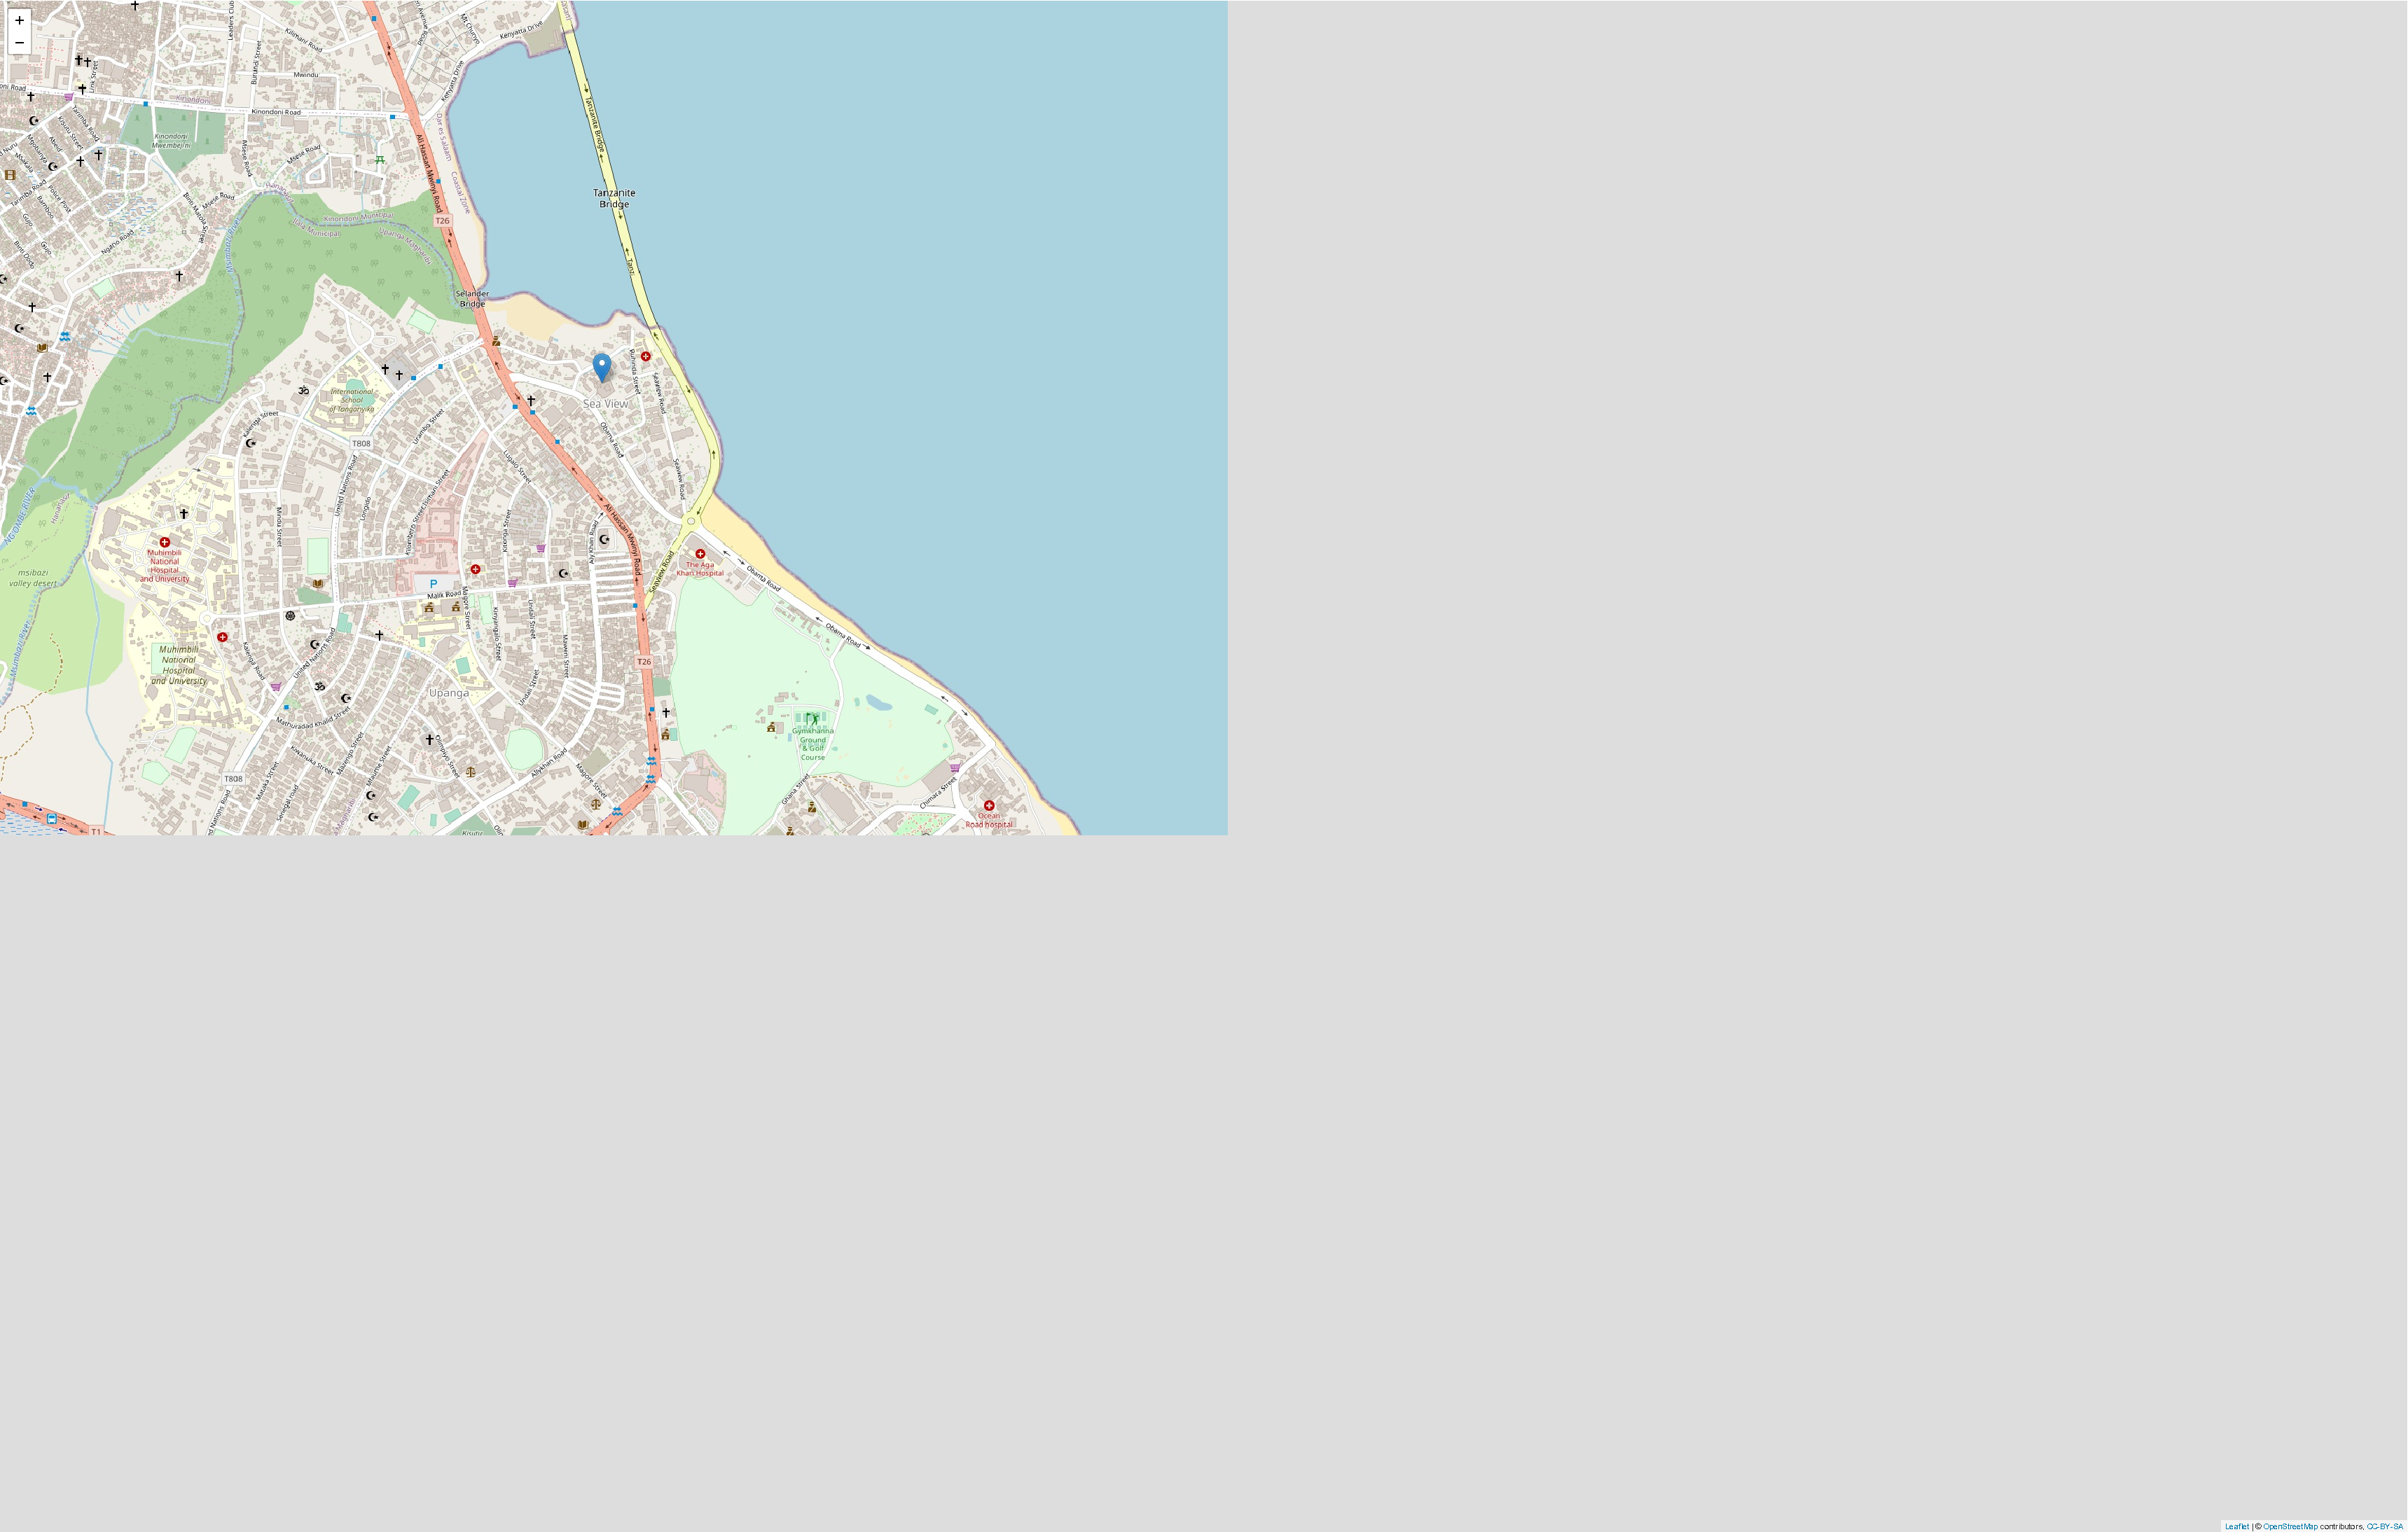
\includegraphics{./intro_files/figure-pdf/unnamed-chunk-1-1.pdf}

\hypertarget{schedule}{%
\section{Schedule}\label{schedule}}

\hypertarget{day-1}{%
\subsection{Day 1}\label{day-1}}

\hypertarget{tbl-day1-schedule}{}
\begin{longtable}[]{@{}
  >{\centering\arraybackslash}p{(\columnwidth - 2\tabcolsep) * \real{0.2222}}
  >{\raggedright\arraybackslash}p{(\columnwidth - 2\tabcolsep) * \real{0.6528}}@{}}
\caption{\label{tbl-day1-schedule}Schedule Day 1}\tabularnewline
\toprule()
\begin{minipage}[b]{\linewidth}\centering
Time
\end{minipage} & \begin{minipage}[b]{\linewidth}\raggedright
Session
\end{minipage} \\
\midrule()
\endfirsthead
\toprule()
\begin{minipage}[b]{\linewidth}\centering
Time
\end{minipage} & \begin{minipage}[b]{\linewidth}\raggedright
Session
\end{minipage} \\
\midrule()
\endhead
08.30 - 09.00 & \begin{minipage}[t]{\linewidth}\raggedright
Welcome\\
Support for software installation\strut
\end{minipage} \\
09.00 - 09.15 & \begin{minipage}[t]{\linewidth}\raggedright
Introduction to data science tools\\
Overview of objectives for Day 1\strut
\end{minipage} \\
09.15 - 10.15 & Version control with Git \\
10.15 - 10.45 & {🍵} {☕} Break \\
10.45 -11.45 & Introduction to dynamic documents and Quarto \\
11.45 - 12.15 & Use Quarto with Stata \\
12.15 - 13.15 & {🍴} Lunch break \\
13.15 - 14.00 & Import external data \\
14.00 - 15.00 & Manipulate data \\
15.00 - 15.30 & {🍵} {☕} Break \\
15.30 - 16.15 & Visualise data \\
16.15 - 17.00 & Share code and collaborate with Git \\
\bottomrule()
\end{longtable}

\hypertarget{day-2}{%
\subsection{Day 2}\label{day-2}}

\hypertarget{tbl-day2-schedule}{}
\begin{longtable}[]{@{}
  >{\centering\arraybackslash}p{(\columnwidth - 2\tabcolsep) * \real{0.1702}}
  >{\raggedright\arraybackslash}p{(\columnwidth - 2\tabcolsep) * \real{0.8298}}@{}}
\caption{\label{tbl-day2-schedule}Schedule Day 2}\tabularnewline
\toprule()
\begin{minipage}[b]{\linewidth}\centering
Time
\end{minipage} & \begin{minipage}[b]{\linewidth}\raggedright
Session (all)
\end{minipage} \\
\midrule()
\endfirsthead
\toprule()
\begin{minipage}[b]{\linewidth}\centering
Time
\end{minipage} & \begin{minipage}[b]{\linewidth}\raggedright
Session (all)
\end{minipage} \\
\midrule()
\endhead
08.30 - 09.00 & Welcome \\
09.00 - 09.20 & \begin{minipage}[t]{\linewidth}\raggedright
Introduction to Data Science for Public Health\\
Overview of objectives for Day 2\strut
\end{minipage} \\
09.20 - 10.15 & Discussion on concepts related to to public health data
for decision-making \\
10.15 - 10.45 & {🍵} {☕} Break \\
10:45-12:15 & Malaria practical \#1 \\
12.15- 13.15 & {🍴} Lunch break \\
13.15- 13.30 & Prepare presentation of data findings \\
13.30 - 14.00 & Present and discuss data findings \\
14.00 - 14.30 & Interdisciplinary discussion on malaria, dataset,
uncertainties, challenges \\
14.00 - 14.30 & Malaria practical \#2 \\
15.00 - 15.30 & {🍵} {☕} Break \\
15.30 - 16.15 & Malaria practical \#2 \\
16.15 - 16.30 & Prepare presentation of data findings \\
16.30 - 17.00 & Present and discuss data findings \\
\bottomrule()
\end{longtable}

\hypertarget{day-3}{%
\subsection{Day 3}\label{day-3}}

\hypertarget{tbl-day3-schedule}{}
\begin{longtable}[]{@{}
  >{\centering\arraybackslash}p{(\columnwidth - 2\tabcolsep) * \real{0.1905}}
  >{\raggedright\arraybackslash}p{(\columnwidth - 2\tabcolsep) * \real{0.8095}}@{}}
\caption{\label{tbl-day3-schedule}Schedule Day 3}\tabularnewline
\toprule()
\begin{minipage}[b]{\linewidth}\centering
Time
\end{minipage} & \begin{minipage}[b]{\linewidth}\raggedright
Session (all)
\end{minipage} \\
\midrule()
\endfirsthead
\toprule()
\begin{minipage}[b]{\linewidth}\centering
Time
\end{minipage} & \begin{minipage}[b]{\linewidth}\raggedright
Session (all)
\end{minipage} \\
\midrule()
\endhead
08.30 - 09.00 & Welcome \\
09.00 - 09.20 & Interdisciplinary introduction to big data and machine
Learning

Overview of objectives for Day 3 \\
09.20 - 10.15 & Discussion on secondary data sources

(Public Datasets, e.g.~DHS, Facebook, facilities, etc)

Benefits and drawbacks between primary and secondary data sources \\
10.15 - 10.45 & {🍵} {☕} Break \\
10.45 - 12.15 & \begin{minipage}[t]{\linewidth}\raggedright
{[}Analysis stream{]} Introduction to machine learning\\
{[}Interpretation stream{]} Critically discuss data
surveys/reports\strut
\end{minipage} \\
12:15-13:15 & {🍴} Lunch break \\
13:15-13:45 & Speed talks - research presentations \\
13:45-15.00 & \begin{minipage}[t]{\linewidth}\raggedright
{[}Analysis stream{]} Data practical\\
{[}Interpretation stream{]} Critically discuss data
surveys/reports\strut
\end{minipage} \\
15.00 - 15.30 & {🍵} {☕} Break \\
15:30-16:00 & Feedback on findings from practicals \\
\begin{minipage}[t]{\linewidth}\centering
16:00-16:30\\
\strut
\end{minipage} & Feedback on workshop - Wrap-up \\
\bottomrule()
\end{longtable}

\hypertarget{to-do-after-the-workshop}{%
\section{To do after the workshop}\label{to-do-after-the-workshop}}

\begin{enumerate}
\def\labelenumi{\arabic{enumi}.}
\tightlist
\item
  Fill out the online post-workshop questionnaire.
\item
  This material will stay online, do not hesitate to refer to it if
  needed.
\end{enumerate}

\part{------------ DAY 1 ------------}

\hypertarget{tools-for-reproducible-quantitative-research}{%
\chapter{\texorpdfstring{{📚} Tools for reproducible quantitative
research}{📚 Tools for reproducible quantitative research}}\label{tools-for-reproducible-quantitative-research}}

\hypertarget{overview}{%
\subsection{Overview}\label{overview}}

When reporting scientific results, researchers must document the steps
they followed so that independent researchers within the broader
research community are able to trust and build upon their findings
(\emph{cumulative knowledge}).

\begin{tcolorbox}[enhanced jigsaw, colframe=quarto-callout-important-color-frame, colback=white, rightrule=.15mm, bottomrule=.15mm, left=2mm, arc=.35mm, coltitle=black, title=\textcolor{quarto-callout-important-color}{\faExclamation}\hspace{0.5em}{Important}, opacitybacktitle=0.6, bottomtitle=1mm, opacityback=0, toptitle=1mm, toprule=.15mm, colbacktitle=quarto-callout-important-color!10!white, titlerule=0mm, leftrule=.75mm, breakable]
Reporting should include negative results as they contribute to the
development of a cumulative knowledge as much as positive results do and
avoid wasting resources.
\end{tcolorbox}

\begin{figure}

{\centering 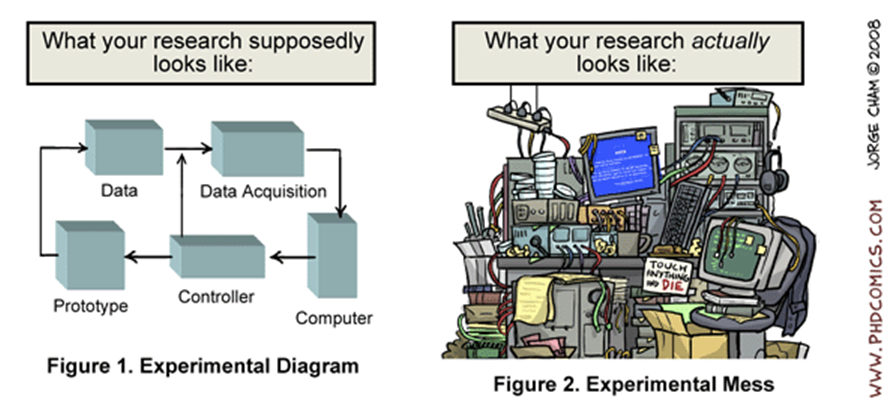
\includegraphics{./images/paste-95377789.png}

}

\caption{\label{fig-research-diagram-vs-research-reality}Research
Diagram vs.~Research Reality. ``Piled Higher and Deeper'' by Jorge Cham
www.phdcomics.com}

\end{figure}

There have been recurrent calls in the recent decades for the scientific
community to embrace practices to support research reproducibility and
many software tools are now available to facilitate this process.

\hypertarget{learning-objectives-1}{%
\subsection{Learning objectives}\label{learning-objectives-1}}

\begin{itemize}
\tightlist
\item
  What is meant by \emph{reproducible quantitative research} and why
  does it matters?
\item
  What should be documented for ensuring the reproducibility of
  quantitative analyses?
\item
  What software tools are available to support reproducible quantitative
  research?
\end{itemize}

\hypertarget{reproducible-quantitative-research}{%
\section{Reproducible quantitative
research}\label{reproducible-quantitative-research}}

A quantitative analysis is said to be (\emph{computationally})
\textbf{reproducible} when the \textbf{same analysis steps} performed on
the \textbf{same dataset} consistently produce the \textbf{same
quantitative results} (1). Given the deterministic nature of computer
programmes, a quantitative analysis must be reproducible to be
\textbf{credible}.

\begin{figure}

{\centering 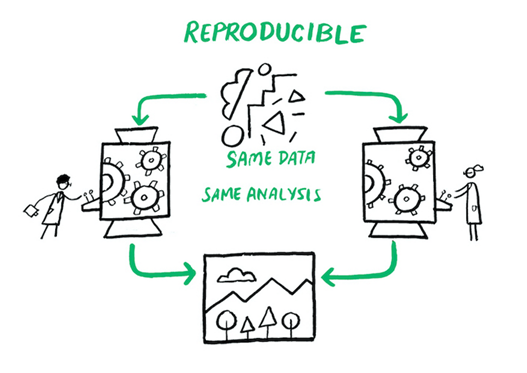
\includegraphics[width=4.16667in,height=\textheight]{./images/paste-97E0048A.png}

}

\caption{\label{fig-reproducibility}This image was created by Scriberia
for The Turing Way community and is used under a CC-BY licence. DOI:
10.5281/zenodo.3332807}

\end{figure}

In addition to (computational) reproducibility, \textbf{replicability},
\textbf{robustness} and \textbf{generalisability} are key to the
generation of strong quantitative evidence.

\hypertarget{replicability}{%
\subsubsection{Replicability}\label{replicability}}

The \textbf{same analysis} steps are performed on \textbf{different
datasets} and produce \textbf{qualitatively similar answers} (1).

\begin{figure}

{\centering 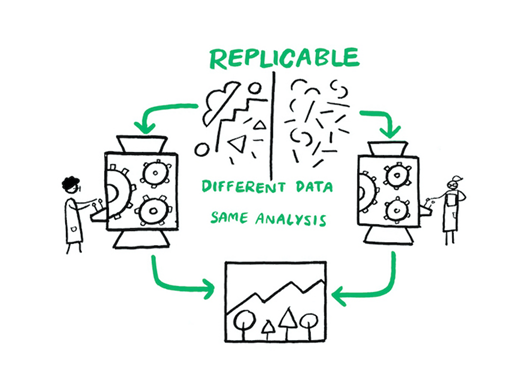
\includegraphics[width=4.16667in,height=\textheight]{./images/paste-5D367441.png}

}

\caption{\label{fig-replicability}This image was created by Scriberia
for The Turing Way community and is used under a CC-BY licence. DOI:
10.5281/zenodo.3332807}

\end{figure}

\hypertarget{robustness}{%
\subsubsection{Robustness}\label{robustness}}

\textbf{Different analysis} steps are performed on the \textbf{same
dataset} to answer the \textbf{same research question} and produce
\textbf{qualitatively similar or identical answers} (1).

\begin{figure}

{\centering 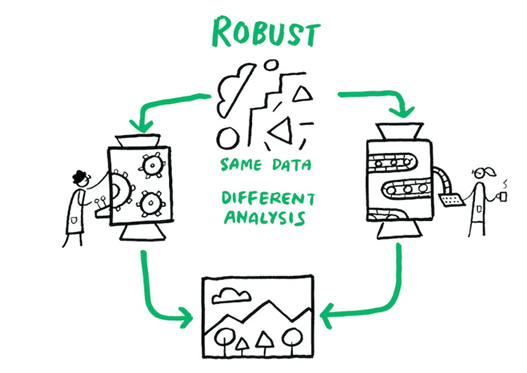
\includegraphics[width=4.16667in,height=\textheight]{./images/paste-1E28AEDC.png}

}

\caption{\label{fig-robustness}This image was created by Scriberia for
The Turing Way community and is used under a CC-BY licence. DOI:
10.5281/zenodo.3332807}

\end{figure}

\hypertarget{generalisability}{%
\subsubsection{Generalisability}\label{generalisability}}

\textbf{Different analysis} steps are performed on the \textbf{different
datasets} to know how well the work applies to all the different aspects
of the research question and produce \textbf{generalisable answers} (1).

\begin{figure}

{\centering 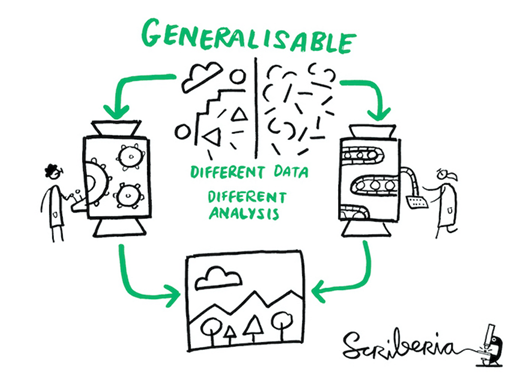
\includegraphics[width=4.16667in,height=\textheight]{./images/paste-222EF473.png}

}

\caption{\label{fig-generalisability}This image was created by Scriberia
for The Turing Way community and is used under a CC-BY licence. DOI:
10.5281/zenodo.3332807}

\end{figure}

\hypertarget{good-documentation-for-reproducible-analyses}{%
\section{Good documentation for reproducible
analyses}\label{good-documentation-for-reproducible-analyses}}

To guarantee that any other researcher can reproduce your analysis, you
would need to document and share the full \textbf{computational
environment}, \textbf{tools}, \textbf{data} and \textbf{code} that were
used to generate your results.

\begin{figure}

{\centering 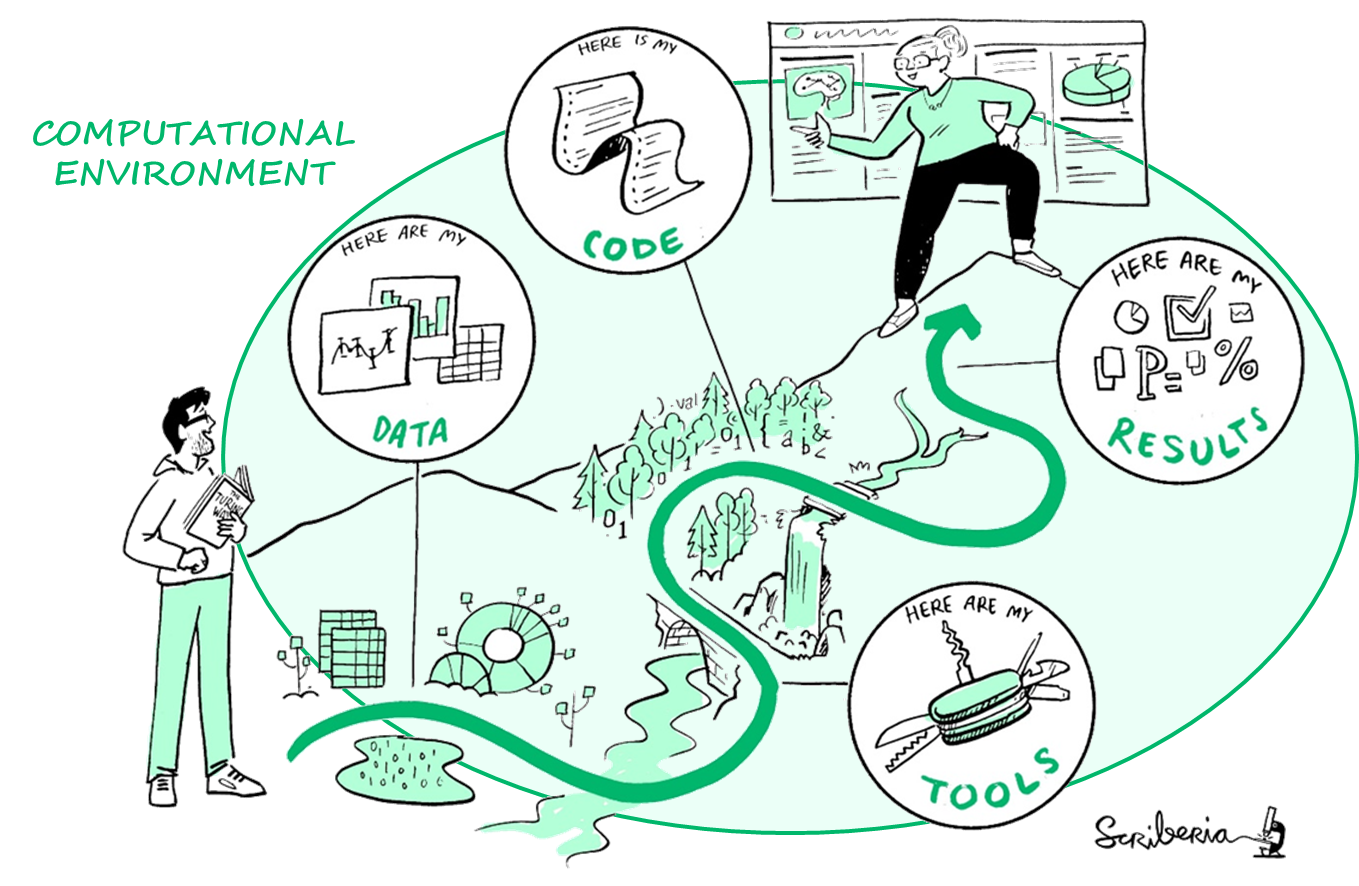
\includegraphics{./images/paste-E04E255A.png}

}

\caption{\label{fig-documentation-reproducible-analysis}This image was
adapted from an original image created by Scriberia for The Turing Way
community (CC-BY licence. DOI: 10.5281/zenodo.3332807).}

\end{figure}

\hypertarget{opportunities-and-challenges-of-reproducible-research}{%
\section{Opportunities and challenges of reproducible
research}\label{opportunities-and-challenges-of-reproducible-research}}

\hypertarget{discussion}{%
\subsubsection{\texorpdfstring{{💬}
Discussion}{💬 Discussion}}\label{discussion}}

\begin{enumerate}
\def\labelenumi{\arabic{enumi}.}
\tightlist
\item
  How do you think reproducible quantitative analyses can improve your
  research?
\item
  Recent investigations have shown that a significant percentage of
  scientific studies cannot be reproduced, thus contributing to growing
  mistrust in scientific results (2,3). What barriers and challenges to
  reproducible research do you see in your daily practice?
\end{enumerate}

{🕒} 5 minutes

\hypertarget{opportunities}{%
\subsubsection{\texorpdfstring{{➕}
Opportunities}{➕ Opportunities}}\label{opportunities}}

\begin{figure}

{\centering 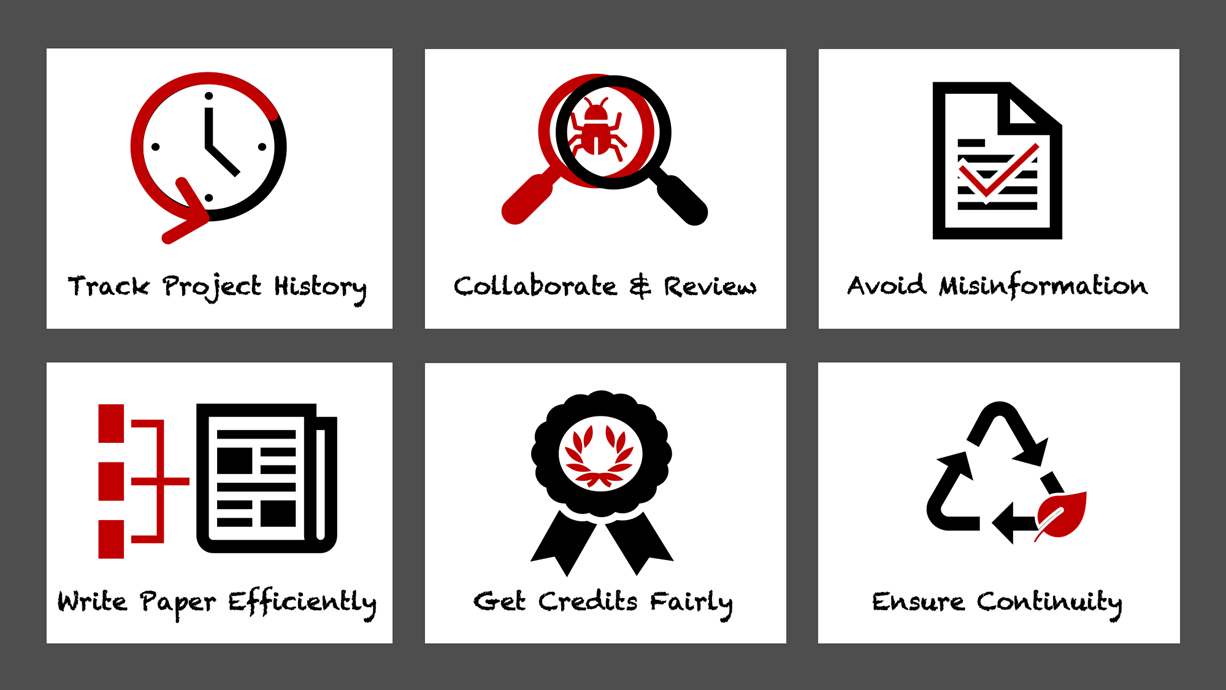
\includegraphics{./images/paste-9DF4B400.png}

}

\caption{This image was created by Scriberia for The Turing Way
community and is used under a CC-BY licence. DOI:
10.5281/zenodo.3332807}

\end{figure}

\hypertarget{barriers-and-challenges}{%
\subsubsection{\texorpdfstring{{➖} Barriers and
challenges}{➖ Barriers and challenges}}\label{barriers-and-challenges}}

\begin{figure}

{\centering 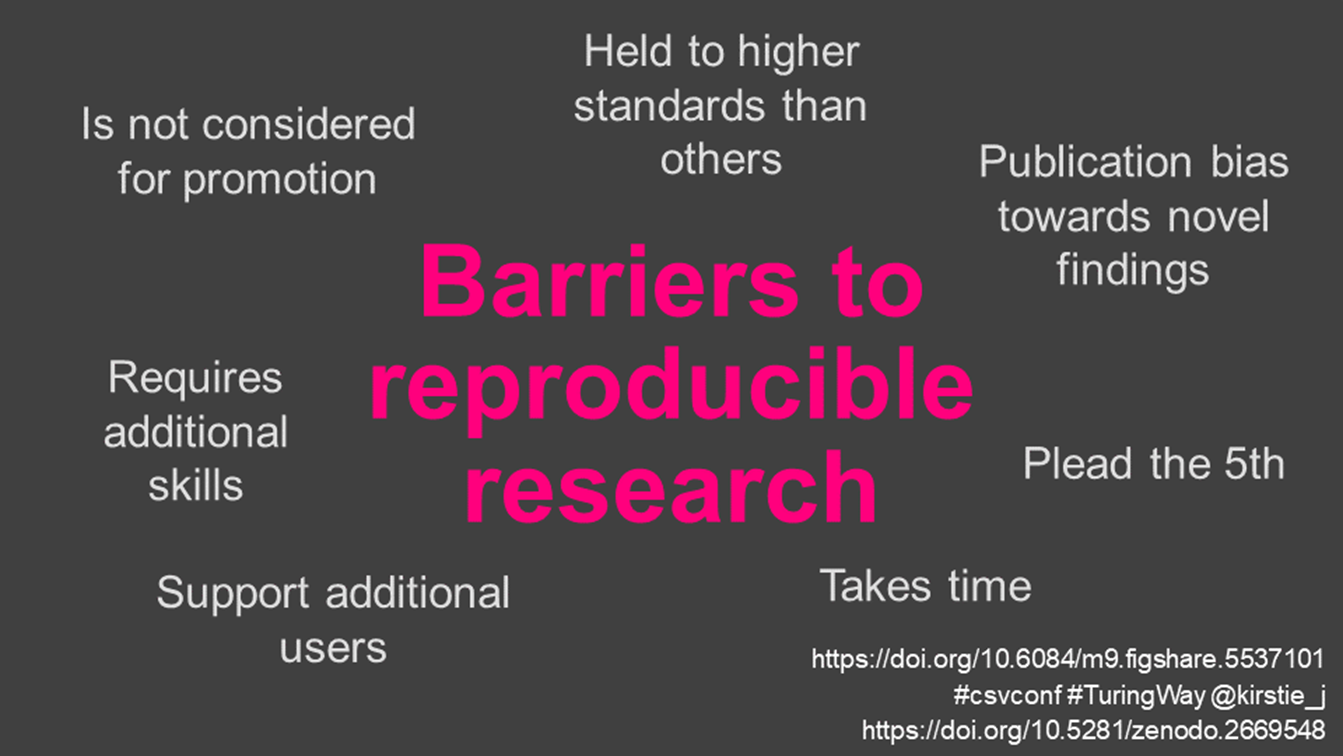
\includegraphics{./images/paste-80DE769E.png}

}

\caption{\label{fig-barriers-reproducibility}Example of barriers to
reproducibility}

\end{figure}

\hypertarget{challenges}{%
\subsubsection{Challenges}\label{challenges}}

In practice, reproducibility is challenging, even for trained data
scientists equipped with an arsenal of software tools. Quantitative
analyses can often not be fully reproduced because of complexities in
how software tools are packaged, installed, and executed and because of
limitations associated with how scientists document analysis steps.

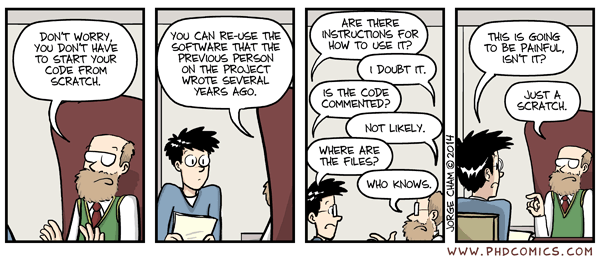
\includegraphics{./images/phd_comics_code_documentation.png}

\hypertarget{software-tools-across-the-research-data-lifecycle}{%
\section{Software tools across the research data
lifecycle}\label{software-tools-across-the-research-data-lifecycle}}

As illustrated in
Figure~\ref{fig-software-tools-across-research-lifecycle}, there is now
a whole set of free or open source software tools that are available to
help you automate your processes and overcome reproducibility challenges
across the research data lifecycle.

In this workshop, you will be introduced to following software tools
that will help make your quantitative data processing, study and
analysis more reproducible:

\begin{itemize}
\tightlist
\item
  \textbf{Git/GitHub} allow you to keep track of various versions of
  your code, share your code and collaborate with others on code
  development;
\item
  \textbf{R} is a programming language for statistical computing and
  graphics and one of main programming language used for data science
  (with other programming languages such as \textbf{Python} and Julia).
  The ecosystem around R provides an interactive environment for data
  science science workflows, thus making R is a great start for your
  data science journey.
\item
  \textbf{Rstudio} is an integrated development environment (IDE) for R
  that enables an easier use of R.
\item
  \textbf{Quarto} allow you to generate (reproducible) dynamic reports
  to document your data analyses. We will use Quarto within the
  \textbf{R/RStudio} environment.
\end{itemize}

\begin{tcolorbox}[enhanced jigsaw, colframe=quarto-callout-important-color-frame, colback=white, rightrule=.15mm, bottomrule=.15mm, left=2mm, arc=.35mm, coltitle=black, title=\textcolor{quarto-callout-important-color}{\faExclamation}\hspace{0.5em}{Important}, opacitybacktitle=0.6, bottomtitle=1mm, opacityback=0, toptitle=1mm, toprule=.15mm, colbacktitle=quarto-callout-important-color!10!white, titlerule=0mm, leftrule=.75mm, breakable]
In practice, most data scientists use a mix of languages, often at least
R and Python. You will be slightly exposed to R, but the goal of this
workshop is
\end{tcolorbox}

\begin{figure}

{\centering 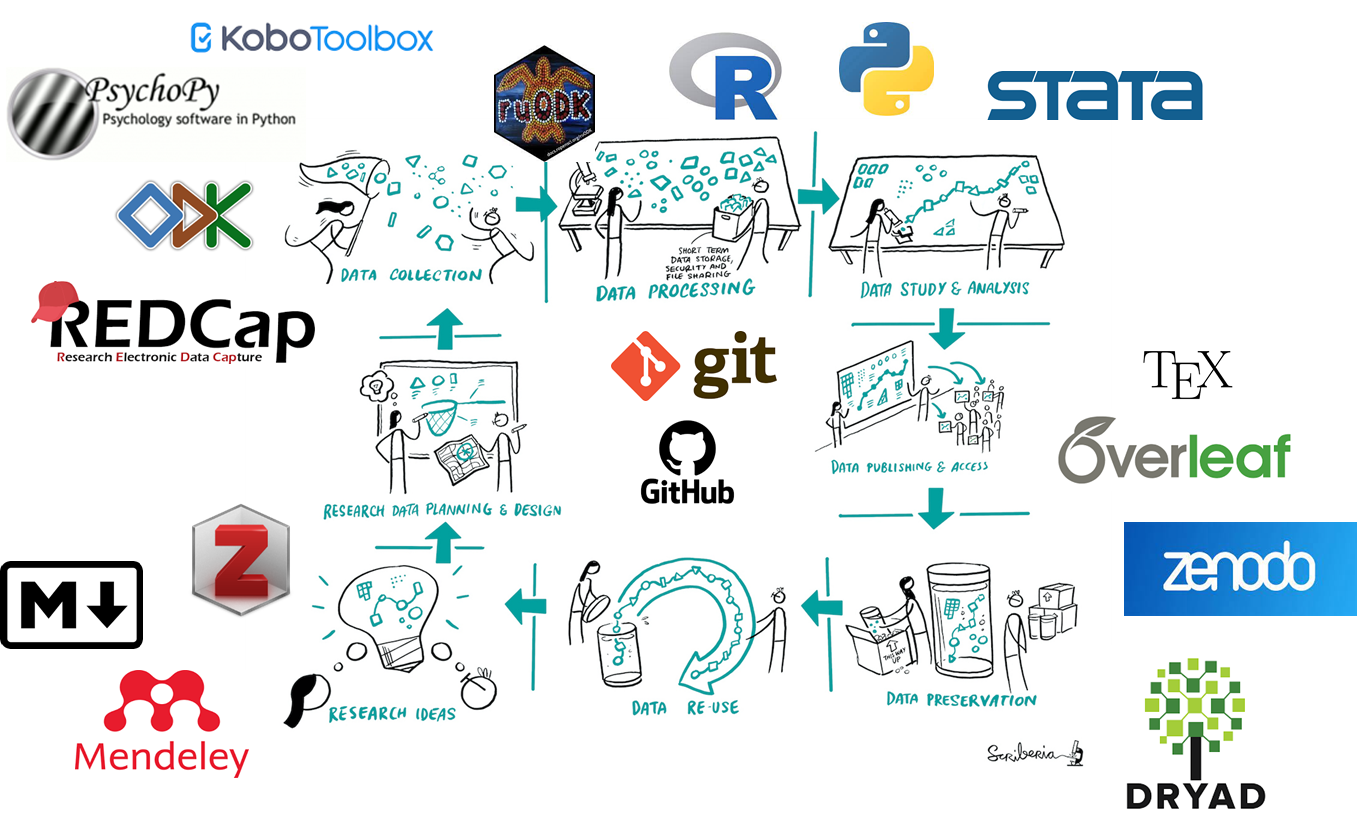
\includegraphics{./images/paste-AF117E41.png}

}

\caption{\label{fig-software-tools-across-research-lifecycle}Example of
free / open source software tools across the research data lifecycle.
This image was adapted from an original image created by Scriberia for
The Turing Way community (CC-BY licence. DOI: 10.5281/zenodo.3332807).}

\end{figure}

\begin{tcolorbox}[enhanced jigsaw, colframe=quarto-callout-note-color-frame, colback=white, rightrule=.15mm, bottomrule=.15mm, left=2mm, arc=.35mm, coltitle=black, title=\textcolor{quarto-callout-note-color}{\faInfo}\hspace{0.5em}{Note}, opacitybacktitle=0.6, bottomtitle=1mm, opacityback=0, toptitle=1mm, toprule=.15mm, colbacktitle=quarto-callout-note-color!10!white, titlerule=0mm, leftrule=.75mm, breakable]
Although qualitative research contributes as significantly as
quantitative research to knowledge generation, the validation of
qualitative research findings is a much more complex and debated concept
as qualitative analysis is by essence subjective and contextual. This
explains the lower availability of software tools dedicated to
qualitative research compared to what is available for quantitative
research.
\end{tcolorbox}

\hypertarget{version-control-with-git}{%
\chapter{\texorpdfstring{{📚} Version control with
Git}{📚 Version control with Git}}\label{version-control-with-git}}

\hypertarget{overview-1}{%
\subsection{Overview}\label{overview-1}}

Does the following situation seem sadly familiar? The challenge here is
not only that you have no idea which draft is actually the latest
version of the document, but also that it is almost impossible to
understand what decision on the document content was taken when.

\begin{figure}

{\centering 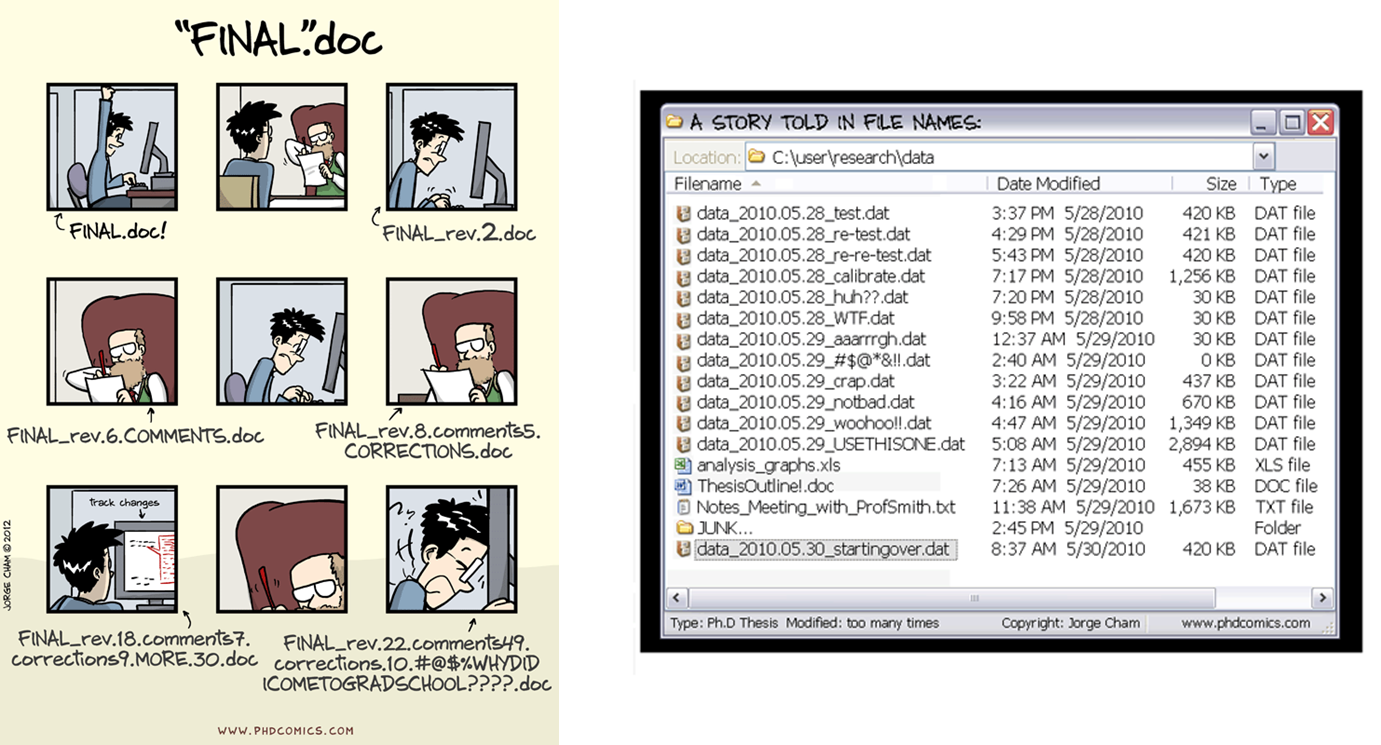
\includegraphics{./images/paste-2840AEE3.png}

}

\caption{\label{fig-final-doc}``Piled Higher and Deeper'' by Jorge Cham
www.phdcomics.com}

\end{figure}

Version control is the process by which the development of a document is
clearly identified. It provides huge benefits to organization,
archiving, and being able to find your files easily when you need them.
Git is a tool that

\hypertarget{learning-objectives-2}{%
\subsection{Learning objectives}\label{learning-objectives-2}}

In this chapter, we introduce the basic elements of version control. We
will learn the terminology and practice version control on a
\emph{need-to-know} basis across the workshop.

\begin{itemize}
\item
  What is version control?
\item
  What tools are available to support version control?
\item
  How to set up Git version control for a project?
\end{itemize}

\hypertarget{version-control}{%
\section{Version control}\label{version-control}}

Version control generally applies at a level of a project. It tracks and
manages different drafts and versions for each document in the project.

\begin{tcolorbox}[enhanced jigsaw, colframe=quarto-callout-important-color-frame, colback=white, rightrule=.15mm, bottomrule=.15mm, left=2mm, arc=.35mm, coltitle=black, title=\textcolor{quarto-callout-important-color}{\faExclamation}\hspace{0.5em}{Important}, opacitybacktitle=0.6, bottomtitle=1mm, opacityback=0, toptitle=1mm, toprule=.15mm, colbacktitle=quarto-callout-important-color!10!white, titlerule=0mm, leftrule=.75mm, breakable]
With version control, you will only see a single file, which is the most
recent version (\emph{final} version). This helps avoiding confusion.
\end{tcolorbox}

Version control provides an audit trail for the revisions and updates of
final versions.

\begin{tcolorbox}[enhanced jigsaw, colframe=quarto-callout-tip-color-frame, colback=white, rightrule=.15mm, bottomrule=.15mm, left=2mm, arc=.35mm, coltitle=black, title=\textcolor{quarto-callout-tip-color}{\faLightbulb}\hspace{0.5em}{Tip}, opacitybacktitle=0.6, bottomtitle=1mm, opacityback=0, toptitle=1mm, toprule=.15mm, colbacktitle=quarto-callout-tip-color!10!white, titlerule=0mm, leftrule=.75mm, breakable]
Version control tracks \textbf{what} changes have been made, \textbf{by
whom} and \textbf{when}, so that you do no longer need to save a copy of
your documents with your name or the date in the filename.
\end{tcolorbox}

Version control allows you to discard recent updates and restore an
earlier version of our project if needed.

\begin{figure}

{\centering 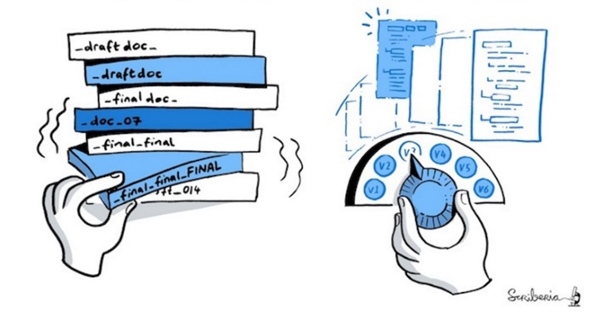
\includegraphics{./images/paste-EB447856.png}

}

\caption{This image was created by Scriberia for The Turing Way
community and is used under a CC-BY licence. DOI:
10.5281/zenodo.3332807}

\end{figure}

\hypertarget{git-github-and-github-desktop}{%
\section{Git, GitHub and GitHub
Desktop}\label{git-github-and-github-desktop}}

\begin{longtable}[]{@{}
  >{\centering\arraybackslash}p{(\columnwidth - 4\tabcolsep) * \real{0.2329}}
  >{\centering\arraybackslash}p{(\columnwidth - 4\tabcolsep) * \real{0.2329}}
  >{\raggedright\arraybackslash}p{(\columnwidth - 4\tabcolsep) * \real{0.5342}}@{}}
\toprule()
\endhead

\includegraphics{./images/paste-5B5DE956.png} & \textbf{Git} & Free and
open programme that tracks changes to your files over time. \\

\includegraphics{./images/paste-A0B6FCC4.png} & \textbf{GitHub} &
Cloud-based hosting platform that lets you host and manage Git
repositories. GitHub synchronizes your local files online and enables
you to collaborate with others (and yourself). \\

\includegraphics[width=1.25in,height=\textheight]{./images/paste-B8632B75.png}
& \textbf{GitHub Desktop} & Application that allows to use Git commands
seamlessly through a visual interface instead of using the command line
(for software developers) or GitHub's website. \\
\bottomrule()
\end{longtable}

We will always use these three tools together.

Please refer to the following sections for instructions on
creation/installation steps:

\begin{itemize}
\tightlist
\item
  Create a GitHub account (\textbf{?@sec-GitHub-account-creation})
\item
  Install GitHub Desktop (Section~\ref{sec-GitHub-Desktop-installation})
\end{itemize}


\includegraphics{./images/paste-081F7F03.png}

\hypertarget{set-up-git-version-control-for-a-project}{%
\section{Set up Git version control for a
project}\label{set-up-git-version-control-for-a-project}}

\begin{tcolorbox}[enhanced jigsaw, colframe=quarto-callout-note-color-frame, colback=white, rightrule=.15mm, bottomrule=.15mm, left=2mm, arc=.35mm, coltitle=black, title=\textcolor{quarto-callout-note-color}{\faInfo}\hspace{0.5em}{Note}, opacitybacktitle=0.6, bottomtitle=1mm, opacityback=0, toptitle=1mm, toprule=.15mm, colbacktitle=quarto-callout-note-color!10!white, titlerule=0mm, leftrule=.75mm, breakable]
A \textbf{repository} is a database of all changes in your project. You
will have a personal copy of all the final versions of the documents in
the project (\emph{working copy}) which will appear on your computer as
a folder.
\end{tcolorbox}

\hypertarget{step-1}{%
\subsubsection{Step 1}\label{step-1}}

Open GitHub Desktop

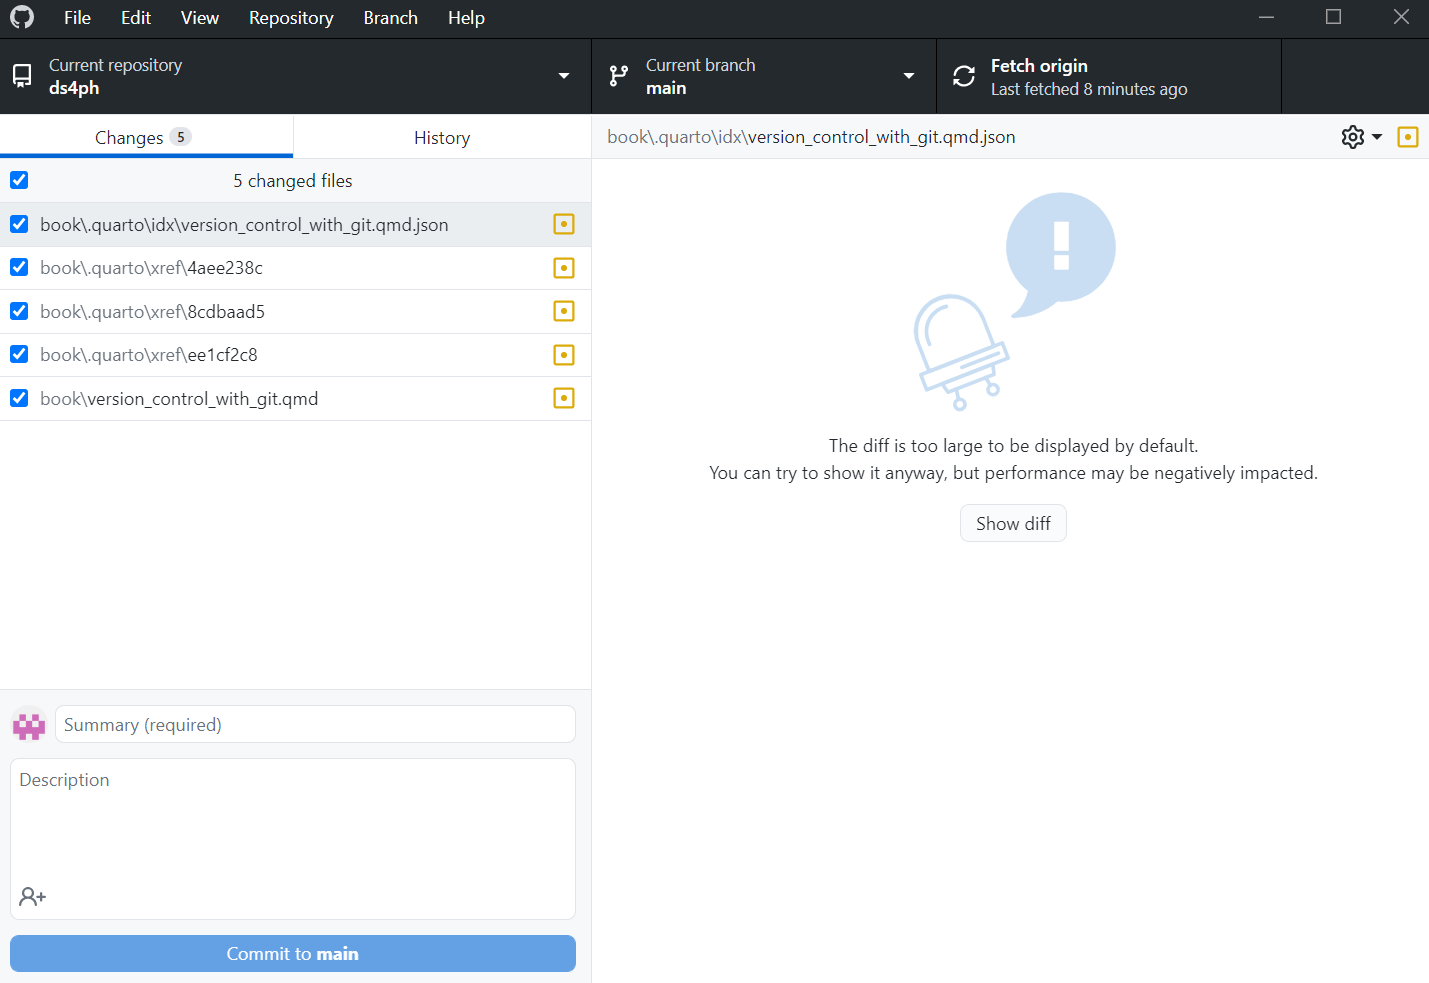
\includegraphics{./images/paste-EFF40D72.png}

\hypertarget{step-2}{%
\subsubsection{Step 2}\label{step-2}}

In GitHub Desktop, you can create a new repository by selecting
\textbf{File} \textgreater{} \textbf{New repository}.

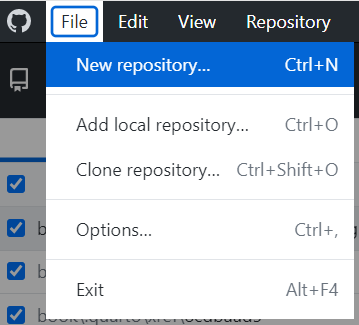
\includegraphics{./images/paste-A85BE0C6.png}

\hypertarget{step-3}{%
\subsubsection{Step 3}\label{step-3}}

\begin{enumerate}
\def\labelenumi{\arabic{enumi}.}
\tightlist
\item
  Enter \textbf{data\_science\_workshop\_sept\_2022} as the name of your
  new repository.
\item
  Click \textbf{Choose\ldots{}} to select the local directory in which
  your new repository will be created. Using Windows Explorer, navigate
  to the local repository of your choice.
\item
  Check \textbf{Initialize this repository with a README} to create a
  README file in your new repository. This is \emph{optional} and you
  will be able to create a README file later if you wish to do so.
\item
  Click on \textbf{Create repository}.
\end{enumerate}

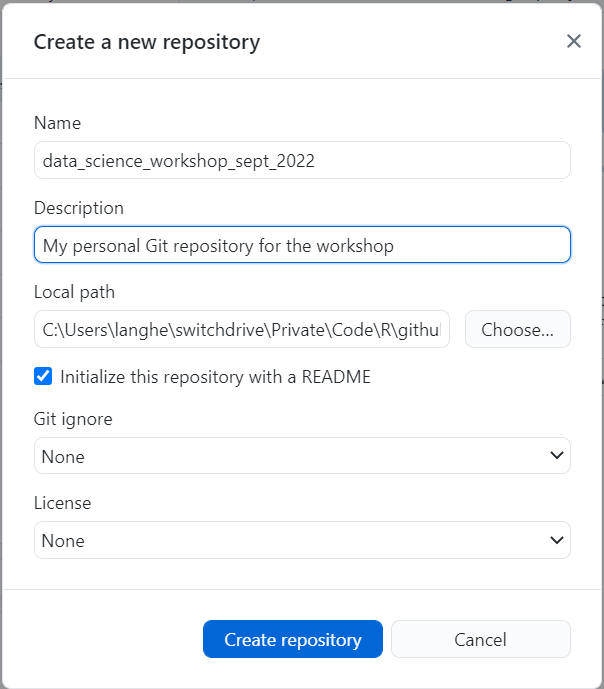
\includegraphics{./images/paste-D831B36F.png}

\hypertarget{to-go-further}{%
\section{To go further}\label{to-go-further}}

To learn more about Git, we refer you to the resources listed in
Section~\ref{sec-resources-git}.

\hypertarget{getting-started-with-rstudio}{%
\chapter{\texorpdfstring{{📘} Getting started with
RStudio}{📘 Getting started with RStudio}}\label{getting-started-with-rstudio}}

\hypertarget{overview-2}{%
\subsection{Overview}\label{overview-2}}

Please review the following sections for instructions on installation
steps:

\begin{itemize}
\tightlist
\item
  Downloading R (\textbf{?@sec-R-installation})
\item
  Downloading and configuring RStudio
  (Section~\ref{sec-RStudio-installation})
\end{itemize}

\hypertarget{learning-objectives-3}{%
\subsection{Learning objectives}\label{learning-objectives-3}}

\begin{enumerate}
\def\labelenumi{\arabic{enumi}.}
\tightlist
\item
  Familiarise with RStudio
\item
  Get set up with not storing the RStudio workspace
\end{enumerate}

\hypertarget{orientation-to-the-rstudio-interface}{%
\section{Orientation to the RStudio
interface}\label{orientation-to-the-rstudio-interface}}

Open RStudio

By default RStudio displays four rectangle panes.

\begin{tcolorbox}[enhanced jigsaw, colframe=quarto-callout-tip-color-frame, colback=white, rightrule=.15mm, bottomrule=.15mm, left=2mm, arc=.35mm, coltitle=black, title=\textcolor{quarto-callout-tip-color}{\faLightbulb}\hspace{0.5em}{Tip}, opacitybacktitle=0.6, bottomtitle=1mm, opacityback=0, toptitle=1mm, toprule=.15mm, colbacktitle=quarto-callout-tip-color!10!white, titlerule=0mm, leftrule=.75mm, breakable]
If your RStudio displays only one left pane it is because you have no
scripts open yet.
\end{tcolorbox}

\hypertarget{r-console-pane}{%
\subsubsection{R Console Pane}\label{r-console-pane}}

The R Console, by default the left or lower-left pane in R Studio, is
the home of the R ``engine''. This is where the commands are actually
run and non-graphic outputs and error/warning messages appear. You can
directly enter and run commands in the R Console, but realize that these
commands are not saved as they are when running commands from a script.

\begin{tcolorbox}[enhanced jigsaw, colframe=quarto-callout-tip-color-frame, colback=white, rightrule=.15mm, bottomrule=.15mm, left=2mm, arc=.35mm, coltitle=black, title=\textcolor{quarto-callout-tip-color}{\faLightbulb}\hspace{0.5em}{Tip}, opacitybacktitle=0.6, bottomtitle=1mm, opacityback=0, toptitle=1mm, toprule=.15mm, colbacktitle=quarto-callout-tip-color!10!white, titlerule=0mm, leftrule=.75mm, breakable]
This pane is similar to the Stata Command and the Results windows.
\end{tcolorbox}

\hypertarget{source-pane}{%
\subsubsection{Source Pane}\label{source-pane}}

This pane, by default in the upper-left, is space to edit and run your
scripts, including the RMarkdown outbreak and survey templates. This
pane can also display datasets (data frames) for viewing.

\begin{tcolorbox}[enhanced jigsaw, colframe=quarto-callout-tip-color-frame, colback=white, rightrule=.15mm, bottomrule=.15mm, left=2mm, arc=.35mm, coltitle=black, title=\textcolor{quarto-callout-tip-color}{\faLightbulb}\hspace{0.5em}{Tip}, opacitybacktitle=0.6, bottomtitle=1mm, opacityback=0, toptitle=1mm, toprule=.15mm, colbacktitle=quarto-callout-tip-color!10!white, titlerule=0mm, leftrule=.75mm, breakable]
This pane is similar to the Stata Do-file and Data Editor windows.
\end{tcolorbox}

\hypertarget{environment-pane}{%
\subsubsection{Environment Pane}\label{environment-pane}}

This pane, by default the upper-right, is most often used to see brief
summaries of objects in the R Environment in the current session. These
objects could include imported, modified, or created datasets,
parameters you have defined (e.g.~a specific epi week for the analysis),
or vectors or lists you have defined during analysis (e.g.~names of
regions). Click on the arrow next to a dataframe name to see its
variables.

\begin{tcolorbox}[enhanced jigsaw, colframe=quarto-callout-tip-color-frame, colback=white, rightrule=.15mm, bottomrule=.15mm, left=2mm, arc=.35mm, coltitle=black, title=\textcolor{quarto-callout-tip-color}{\faLightbulb}\hspace{0.5em}{Tip}, opacitybacktitle=0.6, bottomtitle=1mm, opacityback=0, toptitle=1mm, toprule=.15mm, colbacktitle=quarto-callout-tip-color!10!white, titlerule=0mm, leftrule=.75mm, breakable]
This pane is similar to the Stata Variables Manager window.
\end{tcolorbox}

\hypertarget{lower-right-pane}{%
\subsubsection{Lower-right pane}\label{lower-right-pane}}

The lower-right pane includes several tabs:

\begin{itemize}
\tightlist
\item
  Files (library of files)
\item
  Plots (display of graphics including maps)
\item
  Packages (available R packages including installation/update options)
\item
  Help
\item
  Viewer
\item
  Presentation.
\end{itemize}

\begin{tcolorbox}[enhanced jigsaw, colframe=quarto-callout-tip-color-frame, colback=white, rightrule=.15mm, bottomrule=.15mm, left=2mm, arc=.35mm, coltitle=black, title=\textcolor{quarto-callout-tip-color}{\faLightbulb}\hspace{0.5em}{Tip}, opacitybacktitle=0.6, bottomtitle=1mm, opacityback=0, toptitle=1mm, toprule=.15mm, colbacktitle=quarto-callout-tip-color!10!white, titlerule=0mm, leftrule=.75mm, breakable]
This pane contains the Stata equivalents of the Plots Manager and
Project Manager windows.
\end{tcolorbox}

\hypertarget{open-a-new-r-project}{%
\section{Open a new R project}\label{open-a-new-r-project}}

In RStudio, you can create a new project by selecting \textbf{File}
\textgreater{} \textbf{New Project\ldots{}}

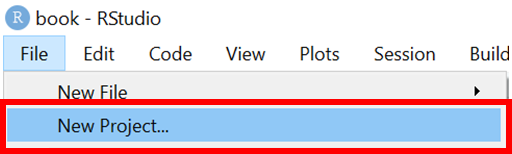
\includegraphics[width=3.64583in,height=\textheight]{./images/paste-CCA1D5A5.png}

Select New Directory

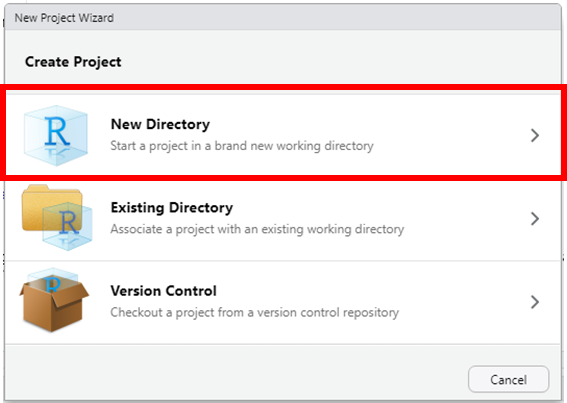
\includegraphics{./images/paste-DCC39BB5.png}

Select New Project

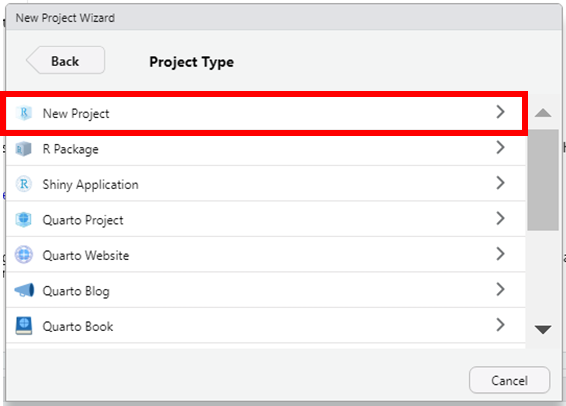
\includegraphics{./images/paste-30A4402B.png}

Select a location to save the new R project (this creates a new folder).

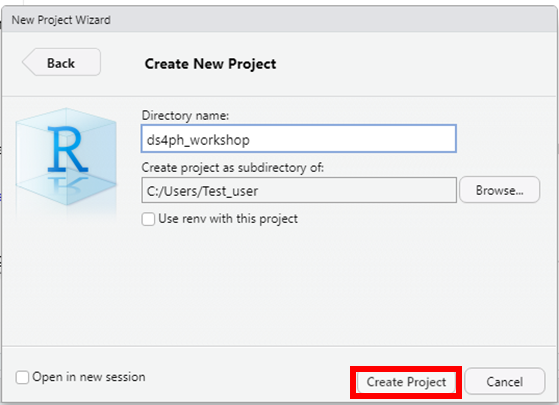
\includegraphics[width=5.20833in,height=\textheight]{./images/paste-C05F97BD.png}

Save all relevant data files into this new R project folder.

We will use this project for the duration of the workshop.

\hypertarget{dynamic-documents}{%
\chapter{\texorpdfstring{{📚} Dynamic
documents}{📚 Dynamic documents}}\label{dynamic-documents}}

\hypertarget{overview-3}{%
\subsection{Overview}\label{overview-3}}

The final product of a quantitative research is a report (e.g.,
scientific publications), i.e.~a textual description of your research
findings along with figures and tables resulting from your analysis.
summary tables and figures. Based on this data, you discuss findings and
give recommendations while using the data as evidence that backs up your
discussion.

Imagine the following situations

\begin{enumerate}
\def\labelenumi{\arabic{enumi}.}
\tightlist
\item
  you are informed that you were given the wrong data set just when you
  have finalised your article for submission to a journal. You are sent
  a new one and you are asked to run the same analysis with this new
  data set.
\item
  you realize that a mistake was made and need to re-examine the code,
  fix the error, and re-run the analysis 3. someone you are training
  wants to see the code and be able to reproduce the results to learn
  about your approach?
\end{enumerate}

Situations like the ones just described are actually quite common for a
data scientist.

It is actually possible to keep your data science projects organized
with RStudio so that re-running an analysis and recreating reports is
straightforward and can be done with minimal effort.Dynamic documents
can be produced to update on a routine basis (e.g.~daily surveillance
reports) and/or run on subsets of data (e.g.~reports for each
jurisdiction).

\hypertarget{learning-objectives-4}{%
\subsection{Learning objectives}\label{learning-objectives-4}}

The goal of this section is to briefly discuss why we want to learn
quarto, the benefits, and the barriers to using it.

\begin{itemize}
\tightlist
\item
  What is a dynamic report?
\item
  What is Quarto?
\item
  Think about why you want to use Quarto
\end{itemize}

\hypertarget{background-to-r-markdown}{%
\section{Background to R Markdown}\label{background-to-r-markdown}}

This is possible due to the fact that Quarto documents enable code and
textual descriptions to be combined into the same document, and the
figures and tables produced by the code are automatically added to the
document.

Quarto is a tool that allows you integrate your code, text and figures
in a single file in order to make high quality, reproducible reports. A
paper published with an included quarto file and data sets can be
reproduced by anyone with a computer. R Markdown integrates code and
natural language in a way that is called ``literate programming'' (4).

To explain some of the concepts and packages involved:

\hypertarget{markdown}{%
\subsubsection{Markdown}\label{markdown}}

Markdown is a ``language'' that allows you to write a document using
plain text, that can be converted to html and other formats. It is not
specific to R.

Markdown files have a \texttt{md} extension.

\hypertarget{r-markdown}{%
\subsubsection{R Markdown}\label{r-markdown}}

It is a variation on markdown that is specific to R - it allows you to
write a document using markdown to produce text and to embed R code and
display their outputs. which was a variant of Markdown specifically
designed to allow R code chunks to be included.

R Markdown is a widely-used tool for creating automated, reproducible,
and share-worthy outputs, such as reports. It can generate static or
interactive outputs, in Word, pdf, html, powerpoint, and other formats.

R Markdown files have \texttt{.Rmd} extension.

\hypertarget{rmarkdown}{%
\subsubsection{rmarkdown}\label{rmarkdown}}

It is the R package: This is used by R to render the .Rmd file into the
desired output.

\hypertarget{quarto}{%
\subsubsection{Quarto}\label{quarto}}

Quarto is the successor to R Markdown. As a R Markdown document, a
Quarto document intersperces code and text such that the script actually
becomes your output document. You can create an entire formatted
document, including narrative text (can be dynamic to change based on
your data), tables, figures, bullets/numbers, bibliographies, etc.

Quatro uses a mark-up language similar to HyperText Markup Language
(HTML) or LaTeX, in comparison to a ``What You See Is What You Get''
(WYSIWYG) language, such as Microsoft Word. This means that all the
aspects are consistent, for instance, all top-level heading will look
the same. But it means that we use symbols to designate how we would
like certain aspects to appear. And it is only when we build the mark-up
that we get to see what it looks like. A visual editor option can also
be used which hides the need for the user to do this mark-up themselves.

Quarto is not tied to the R language.

Quarto files have a \texttt{.Qmd} extension.

\hypertarget{knitr}{%
\subsubsection{knitr}\label{knitr}}

This R package will read the code chunks, execute it, and `knit' it back
into the document. This is how tables and graphs are included alongside
the text.

\hypertarget{pandoc}{%
\subsubsection{Pandoc}\label{pandoc}}

Pandoc actually convert the output into word/pdf/powerpoint etc. It is a
software separate from R but is installed automatically with RStudio.

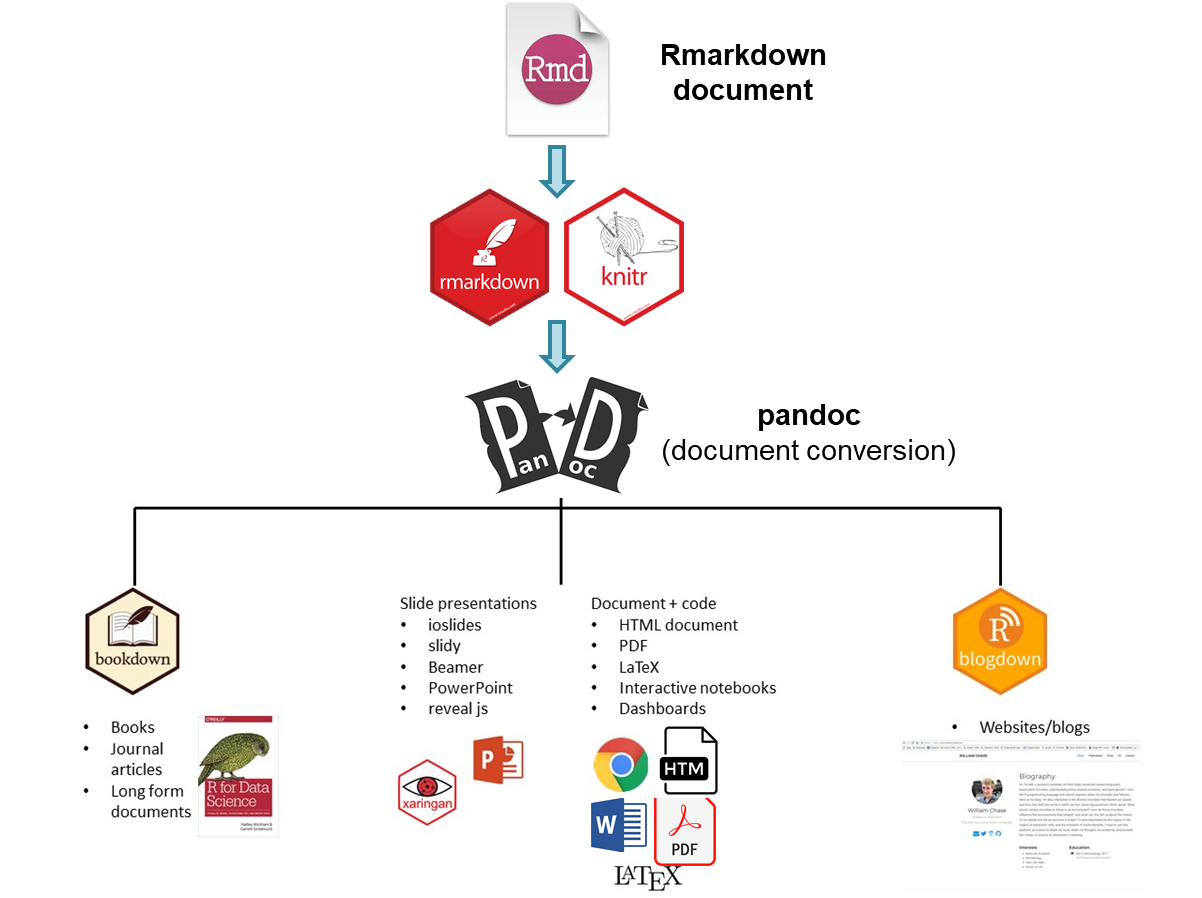
\includegraphics{./images/paste-ABFB521E.png}

The process that happens in the background involves feeding the .Rmd
file to knitr, which executes the R code chunks and creates a new .md
(markdown) file which includes the R code and its rendered output. The
.md file is then processed by Pandoc to create the final product: a
Microsoft Word document, HTML file, PowerPoint document, PDF, etc.

\hypertarget{discussion-1}{%
\subsubsection{\texorpdfstring{{💬}
Discussion}{💬 Discussion}}\label{discussion-1}}

Form small groups of 2-4 with your neighbours and discuss how you expect
learning Quarto might benefit you.

{🕒} 5 minutes

\hypertarget{references}{%
\section{References}\label{references}}

\begin{itemize}
\tightlist
\item
  The Epidemiologist R Handbook (https://epirhandbook.com)
\end{itemize}

\hypertarget{getting-started-with-quarto}{%
\chapter{\texorpdfstring{{📘} Getting started with
Quarto}{📘 Getting started with Quarto}}\label{getting-started-with-quarto}}

\hypertarget{overview-4}{%
\subsection{Overview}\label{overview-4}}

Please review the following sections for instructions on installation
steps:

\begin{itemize}
\tightlist
\item
  Downloading Quarto (Section~\ref{sec-Quarto-installation})
\item
  Installing the rmarkdown package
\end{itemize}

\hypertarget{learning-objectives-5}{%
\subsection{Learning objectives}\label{learning-objectives-5}}

\begin{enumerate}
\def\labelenumi{\arabic{enumi}.}
\tightlist
\item
  Learn how to use Quarto
\end{enumerate}

\hypertarget{create-a-new-quarto-document}{%
\section{Create a new Quarto
document}\label{create-a-new-quarto-document}}

While it makes sense to use Quarto going forward, there are still a lot
of resources written for and in R Markdown. For this reason we provide
the R Markdown equivalents for this section in Appendix.

In RStudio, you can create a new Quarto document by selecting
\textbf{File} \textgreater{} \textbf{New File} \textgreater{}
\textbf{Quarto Document\ldots{}}

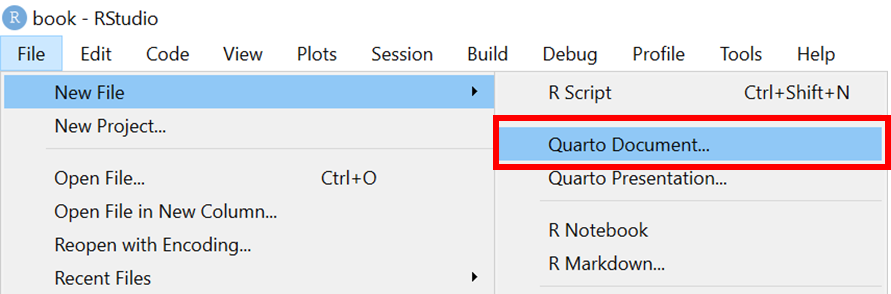
\includegraphics{./images/paste-A7DE8B60.png}

When you create a new Quarto document, RStudio tries to be helpful by
allowing you to select a template which explains the different section
of an R Markdown script. R Studio will enable you select options to pick
from to generate a template Quarto document to start from.

The title and the author names are not important. If the output document
type you want is not one of these, do not worry - you can just pick any
one and change it later.

Let us select \emph{HTML} to create an html document.

Click on create to open up a new Quarto (.Qmd) document.

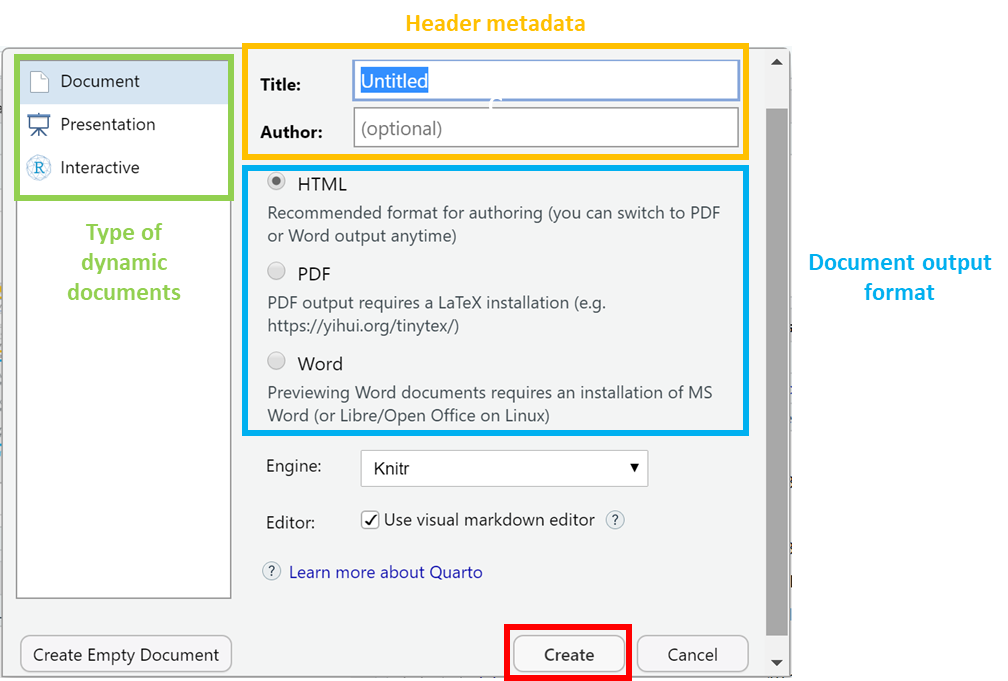
\includegraphics{./images/paste-67B97E04.png}

\hypertarget{visual-editor}{%
\section{Visual Editor}\label{visual-editor}}

The RStudio Visual Editor is quite new and has features that improve
your writing experience. Working in the Visual Editor feels a bit like
working in a Google Doc.

Here's an example showing the same file in the original Source Editor
with content in markdown format and in the Visual Editor with content
that looks more like it will appear in a live site. You can switch
freely between these modes.

\hypertarget{quarto-document-structure}{%
\section{Quarto document structure}\label{quarto-document-structure}}

An R Markdown document can be edited in RStudio.

There are three basic components to a Quarto document, similar to the
components of a R Markdown document:

\begin{itemize}
\tightlist
\item
  metadata (YAML header)
\item
  text (markdown formatting)
\item
  code (R code formatting)
\end{itemize}

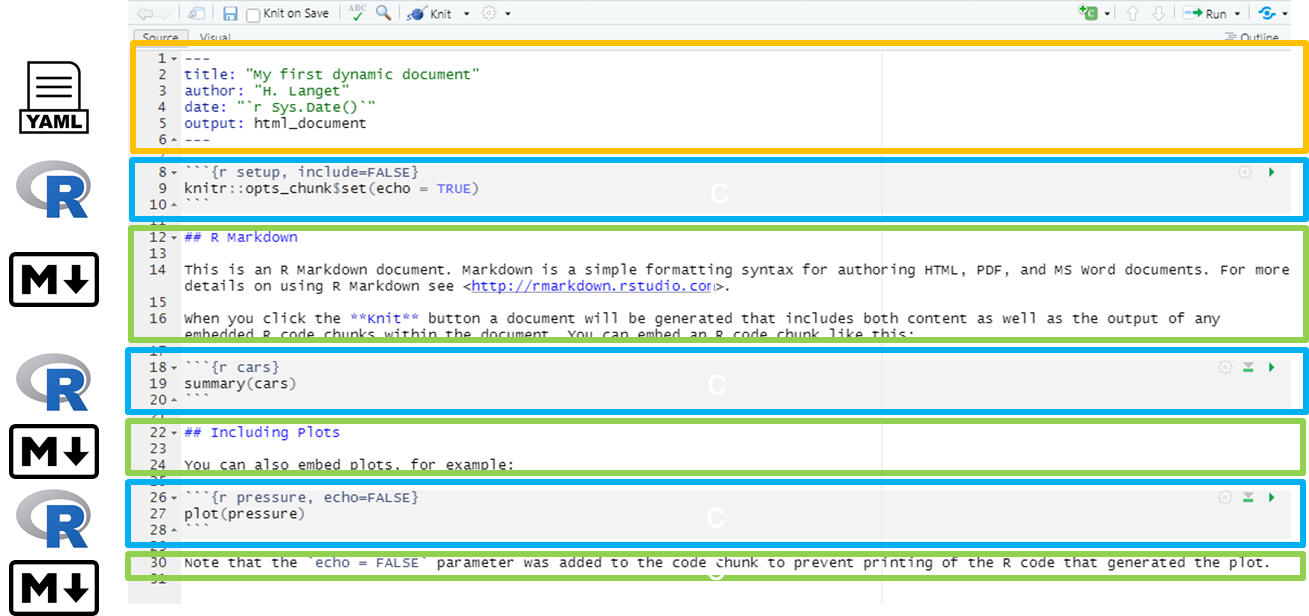
\includegraphics{./images/paste-30C30ECC.png}

\hypertarget{yaml-header}{%
\subsubsection{YAML header}\label{yaml-header}}

The very top of the document consists of a (YAML) header surrounded by
--- lines. Here you may want to edit the title of your document. The
other settings in the header define the default document type produced
(Microsoft Word) when the RMarkdown is ``knit''. the information
intended to produce an html output.

\hypertarget{text}{%
\subsubsection{Text}\label{text}}

In WHITE background areas, any text will appear as regular text in the
final report. Can have formatting such as headings, italics, bold,
numbers, and bullets. See the second page of this RMarkdown cheatsheet
for more detail. Can display parameters derived from your data via
in-line code (such as epi week of the outbreak peak, as in the example
above).

\hypertarget{code-chunks}{%
\subsubsection{Code chunks}\label{code-chunks}}

In gray background ``code chunks'', RMarkdown is running R commands.
These commands perform data processing and cleaning steps, or could
produce visual outputs in the document.

\hypertarget{quarto-render}{%
\section{Quarto render}\label{quarto-render}}

When you click the \textbf{Render} button a document will be generated
that includes both content and the output of embedded code.


\includegraphics{./images/paste-A8386DC4.png} \#\# Code options

You can embed code like this:

\begin{Shaded}
\begin{Highlighting}[]
\DecValTok{1} \SpecialCharTok{+} \DecValTok{1}
\end{Highlighting}
\end{Shaded}

\begin{verbatim}
[1] 2
\end{verbatim}

You can add options to executable code like this

\begin{verbatim}
[1] 4
\end{verbatim}

The \texttt{echo:\ false} option disables the printing of code (only
output is displayed).

\hypertarget{references-1}{%
\section{References}\label{references-1}}

\begin{itemize}
\tightlist
\item
  The Epidemiologist R Handbook (https://epirhandbook.com)
\end{itemize}

\hypertarget{commit-your-changes-with-git}{%
\chapter{\texorpdfstring{{📘} Commit your changes with
Git}{📘 Commit your changes with Git}}\label{commit-your-changes-with-git}}

Version control uses a \emph{working copy} where you do your work.

\begin{tcolorbox}[enhanced jigsaw, colframe=quarto-callout-note-color-frame, colback=white, rightrule=.15mm, bottomrule=.15mm, left=2mm, arc=.35mm, coltitle=black, title=\textcolor{quarto-callout-note-color}{\faInfo}\hspace{0.5em}{Note}, opacitybacktitle=0.6, bottomtitle=1mm, opacityback=0, toptitle=1mm, toprule=.15mm, colbacktitle=quarto-callout-note-color!10!white, titlerule=0mm, leftrule=.75mm, breakable]
You can \texttt{update} your working copy to incorporate any new edits
or versions that have been added to the repository since the last time
you updated.
\end{tcolorbox}

You make arbitrary edits to this copy, without affecting your teammates.
When you are happy with your edits, you \texttt{commit} your changes to
a \emph{repository}.

Snapshot of your entire repository at a specific time.

Over time, commits should tell a story of the history of your repository
and how it came to be the way that it currently is.

Commits include lots of metadata in addition to the contents and
message, like the author, timestamp, and more.

It also requires that you write something human-readable that will be a
breadcrumb for you in the future. be easy to compare versions, and you
can easily revert to previous versions.

\hypertarget{push-and-pull}{%
\section{Push and Pull}\label{push-and-pull}}

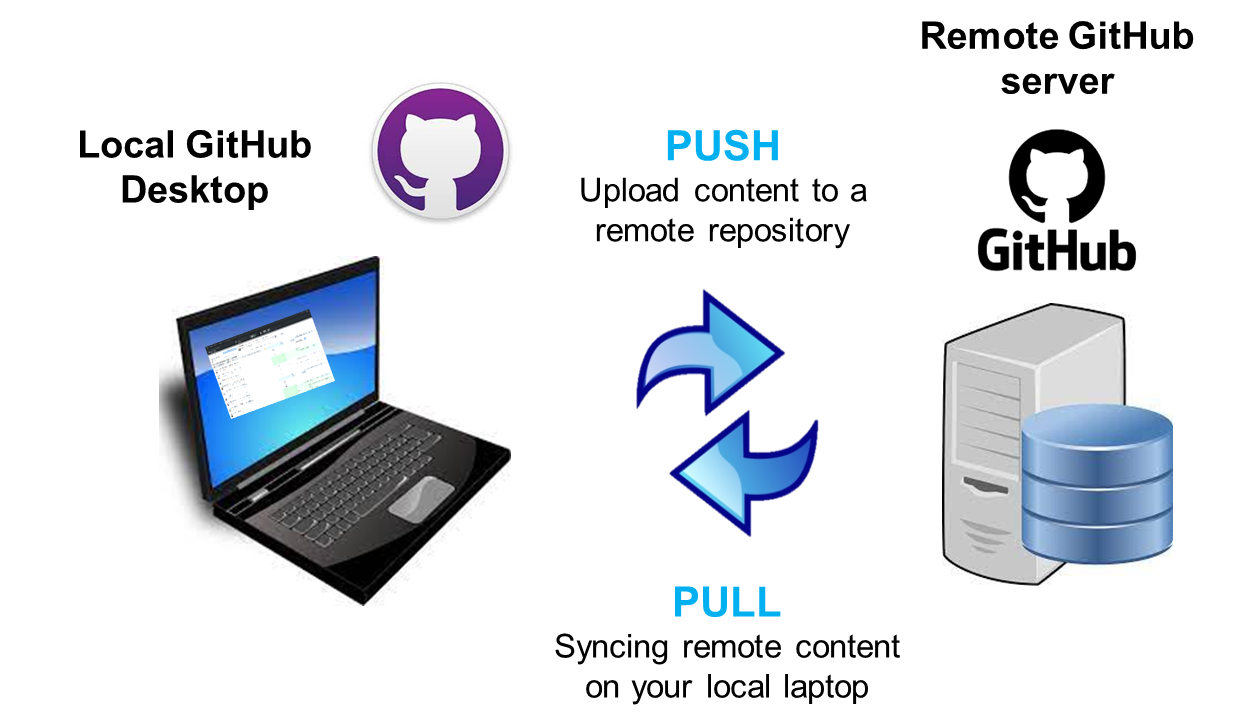
\includegraphics{./images/paste-A340C143.png}

\hypertarget{code-chunks-1}{%
\chapter{\texorpdfstring{{📘} Code
chunks}{📘 Code chunks}}\label{code-chunks-1}}

As the number of programming languages used for scientific discourse is
very broad, Quarto was developed to be multilingual, beginning with R,
Python, Javascript, and Julia. building on the RStudio (R) and Jupyter
(Python, Julia) ecosystems which are very popular.

In this section, we will see how to use and mix R, Stata and Python
within Quarto so that you can make the most out of it.

\hypertarget{create-code-chunks}{%
\section{Create code chunks}\label{create-code-chunks}}

\begin{tcolorbox}[enhanced jigsaw, colframe=quarto-callout-tip-color-frame, colback=white, rightrule=.15mm, bottomrule=.15mm, left=2mm, arc=.35mm, coltitle=black, title=\textcolor{quarto-callout-tip-color}{\faLightbulb}\hspace{0.5em}{Tip}, opacitybacktitle=0.6, bottomtitle=1mm, opacityback=0, toptitle=1mm, toprule=.15mm, colbacktitle=quarto-callout-tip-color!10!white, titlerule=0mm, leftrule=.75mm, breakable]

\begin{itemize}
\tightlist
\item
  Use backticks
\item
  Click on icon
\item
  Keyboard shortcut \texttt{Ctrl} + \texttt{Alt} + \texttt{I}
\end{itemize}

\end{tcolorbox}

\hypertarget{r-code-chunks}{%
\section{R code chunks}\label{r-code-chunks}}

\begin{tcolorbox}[enhanced jigsaw, colframe=quarto-callout-note-color-frame, colback=white, rightrule=.15mm, bottomrule=.15mm, left=2mm, arc=.35mm, coltitle=black, title=\textcolor{quarto-callout-note-color}{\faInfo}\hspace{0.5em}{Note}, opacitybacktitle=0.6, bottomtitle=1mm, opacityback=0, toptitle=1mm, toprule=.15mm, colbacktitle=quarto-callout-note-color!10!white, titlerule=0mm, leftrule=.75mm, breakable]
A \textbf{data frame} is a two-dimensional array-like structure that
contains rows and columns.
\end{tcolorbox}

To store the content of the \emph{iris} data set in data frame
\texttt{df}, you can use \texttt{=} (\emph{equal}) but good practice
recommend using \texttt{\textless{}-} (\emph{back arrow}) to indicate
the direction of your allocation.

\begin{Shaded}
\begin{Highlighting}[]
\InformationTok{\textasciigrave{}\textasciigrave{}\textasciigrave{}\{r\}}
\NormalTok{df }\OtherTok{\textless{}{-}}\NormalTok{ iris}
\InformationTok{\textasciigrave{}\textasciigrave{}\textasciigrave{}}
\end{Highlighting}
\end{Shaded}

How to display data

\begin{Shaded}
\begin{Highlighting}[]
\InformationTok{\textasciigrave{}\textasciigrave{}\textasciigrave{}\{r\}}
\CommentTok{\#| df{-}print: kable}
\FunctionTok{library}\NormalTok{(dplyr)}
\NormalTok{knitr}\SpecialCharTok{::}\FunctionTok{kable}\NormalTok{(}\FunctionTok{head}\NormalTok{(df, }\DecValTok{10}\NormalTok{))}
\InformationTok{\textasciigrave{}\textasciigrave{}\textasciigrave{}}
\end{Highlighting}
\end{Shaded}

\begin{longtable}[]{@{}rrrrl@{}}
\toprule()
Sepal.Length & Sepal.Width & Petal.Length & Petal.Width & Species \\
\midrule()
\endhead
5.1 & 3.5 & 1.4 & 0.2 & setosa \\
4.9 & 3.0 & 1.4 & 0.2 & setosa \\
4.7 & 3.2 & 1.3 & 0.2 & setosa \\
4.6 & 3.1 & 1.5 & 0.2 & setosa \\
5.0 & 3.6 & 1.4 & 0.2 & setosa \\
5.4 & 3.9 & 1.7 & 0.4 & setosa \\
4.6 & 3.4 & 1.4 & 0.3 & setosa \\
5.0 & 3.4 & 1.5 & 0.2 & setosa \\
4.4 & 2.9 & 1.4 & 0.2 & setosa \\
4.9 & 3.1 & 1.5 & 0.1 & setosa \\
\bottomrule()
\end{longtable}

The pipe operator

\begin{Shaded}
\begin{Highlighting}[]
\InformationTok{\textasciigrave{}\textasciigrave{}\textasciigrave{}\{r\}}
\CommentTok{\#| df{-}print: kable}
\FunctionTok{library}\NormalTok{(dplyr)}
\NormalTok{df }\SpecialCharTok{\%\textgreater{}\%}
  \FunctionTok{head}\NormalTok{(}\DecValTok{10}\NormalTok{) }\SpecialCharTok{\%\textgreater{}\%}
\NormalTok{  knitr}\SpecialCharTok{::}\FunctionTok{kable}\NormalTok{()}
\InformationTok{\textasciigrave{}\textasciigrave{}\textasciigrave{}}
\end{Highlighting}
\end{Shaded}

\begin{longtable}[]{@{}rrrrl@{}}
\toprule()
Sepal.Length & Sepal.Width & Petal.Length & Petal.Width & Species \\
\midrule()
\endhead
5.1 & 3.5 & 1.4 & 0.2 & setosa \\
4.9 & 3.0 & 1.4 & 0.2 & setosa \\
4.7 & 3.2 & 1.3 & 0.2 & setosa \\
4.6 & 3.1 & 1.5 & 0.2 & setosa \\
5.0 & 3.6 & 1.4 & 0.2 & setosa \\
5.4 & 3.9 & 1.7 & 0.4 & setosa \\
4.6 & 3.4 & 1.4 & 0.3 & setosa \\
5.0 & 3.4 & 1.5 & 0.2 & setosa \\
4.4 & 2.9 & 1.4 & 0.2 & setosa \\
4.9 & 3.1 & 1.5 & 0.1 & setosa \\
\bottomrule()
\end{longtable}

You can cross-reference your table Table~\ref{tbl-iris}

\begin{Shaded}
\begin{Highlighting}[]
\InformationTok{\textasciigrave{}\textasciigrave{}\textasciigrave{}\{r\}}
\CommentTok{\#| label: tbl{-}iris}
\CommentTok{\#| tbl{-}cap: Iris data set}
\CommentTok{\#| df{-}print: kable}
\NormalTok{df }\SpecialCharTok{\%\textgreater{}\%} 
\NormalTok{  knitr}\SpecialCharTok{::}\FunctionTok{kable}\NormalTok{()}
\InformationTok{\textasciigrave{}\textasciigrave{}\textasciigrave{}}
\end{Highlighting}
\end{Shaded}

\hypertarget{tbl-iris}{}
\begin{longtable}[]{@{}rrrrl@{}}
\caption{\label{tbl-iris}Iris data set}\tabularnewline
\toprule()
Sepal.Length & Sepal.Width & Petal.Length & Petal.Width & Species \\
\midrule()
\endfirsthead
\toprule()
Sepal.Length & Sepal.Width & Petal.Length & Petal.Width & Species \\
\midrule()
\endhead
5.1 & 3.5 & 1.4 & 0.2 & setosa \\
4.9 & 3.0 & 1.4 & 0.2 & setosa \\
4.7 & 3.2 & 1.3 & 0.2 & setosa \\
4.6 & 3.1 & 1.5 & 0.2 & setosa \\
5.0 & 3.6 & 1.4 & 0.2 & setosa \\
5.4 & 3.9 & 1.7 & 0.4 & setosa \\
4.6 & 3.4 & 1.4 & 0.3 & setosa \\
5.0 & 3.4 & 1.5 & 0.2 & setosa \\
4.4 & 2.9 & 1.4 & 0.2 & setosa \\
4.9 & 3.1 & 1.5 & 0.1 & setosa \\
5.4 & 3.7 & 1.5 & 0.2 & setosa \\
4.8 & 3.4 & 1.6 & 0.2 & setosa \\
4.8 & 3.0 & 1.4 & 0.1 & setosa \\
4.3 & 3.0 & 1.1 & 0.1 & setosa \\
5.8 & 4.0 & 1.2 & 0.2 & setosa \\
5.7 & 4.4 & 1.5 & 0.4 & setosa \\
5.4 & 3.9 & 1.3 & 0.4 & setosa \\
5.1 & 3.5 & 1.4 & 0.3 & setosa \\
5.7 & 3.8 & 1.7 & 0.3 & setosa \\
5.1 & 3.8 & 1.5 & 0.3 & setosa \\
5.4 & 3.4 & 1.7 & 0.2 & setosa \\
5.1 & 3.7 & 1.5 & 0.4 & setosa \\
4.6 & 3.6 & 1.0 & 0.2 & setosa \\
5.1 & 3.3 & 1.7 & 0.5 & setosa \\
4.8 & 3.4 & 1.9 & 0.2 & setosa \\
5.0 & 3.0 & 1.6 & 0.2 & setosa \\
5.0 & 3.4 & 1.6 & 0.4 & setosa \\
5.2 & 3.5 & 1.5 & 0.2 & setosa \\
5.2 & 3.4 & 1.4 & 0.2 & setosa \\
4.7 & 3.2 & 1.6 & 0.2 & setosa \\
4.8 & 3.1 & 1.6 & 0.2 & setosa \\
5.4 & 3.4 & 1.5 & 0.4 & setosa \\
5.2 & 4.1 & 1.5 & 0.1 & setosa \\
5.5 & 4.2 & 1.4 & 0.2 & setosa \\
4.9 & 3.1 & 1.5 & 0.2 & setosa \\
5.0 & 3.2 & 1.2 & 0.2 & setosa \\
5.5 & 3.5 & 1.3 & 0.2 & setosa \\
4.9 & 3.6 & 1.4 & 0.1 & setosa \\
4.4 & 3.0 & 1.3 & 0.2 & setosa \\
5.1 & 3.4 & 1.5 & 0.2 & setosa \\
5.0 & 3.5 & 1.3 & 0.3 & setosa \\
4.5 & 2.3 & 1.3 & 0.3 & setosa \\
4.4 & 3.2 & 1.3 & 0.2 & setosa \\
5.0 & 3.5 & 1.6 & 0.6 & setosa \\
5.1 & 3.8 & 1.9 & 0.4 & setosa \\
4.8 & 3.0 & 1.4 & 0.3 & setosa \\
5.1 & 3.8 & 1.6 & 0.2 & setosa \\
4.6 & 3.2 & 1.4 & 0.2 & setosa \\
5.3 & 3.7 & 1.5 & 0.2 & setosa \\
5.0 & 3.3 & 1.4 & 0.2 & setosa \\
7.0 & 3.2 & 4.7 & 1.4 & versicolor \\
6.4 & 3.2 & 4.5 & 1.5 & versicolor \\
6.9 & 3.1 & 4.9 & 1.5 & versicolor \\
5.5 & 2.3 & 4.0 & 1.3 & versicolor \\
6.5 & 2.8 & 4.6 & 1.5 & versicolor \\
5.7 & 2.8 & 4.5 & 1.3 & versicolor \\
6.3 & 3.3 & 4.7 & 1.6 & versicolor \\
4.9 & 2.4 & 3.3 & 1.0 & versicolor \\
6.6 & 2.9 & 4.6 & 1.3 & versicolor \\
5.2 & 2.7 & 3.9 & 1.4 & versicolor \\
5.0 & 2.0 & 3.5 & 1.0 & versicolor \\
5.9 & 3.0 & 4.2 & 1.5 & versicolor \\
6.0 & 2.2 & 4.0 & 1.0 & versicolor \\
6.1 & 2.9 & 4.7 & 1.4 & versicolor \\
5.6 & 2.9 & 3.6 & 1.3 & versicolor \\
6.7 & 3.1 & 4.4 & 1.4 & versicolor \\
5.6 & 3.0 & 4.5 & 1.5 & versicolor \\
5.8 & 2.7 & 4.1 & 1.0 & versicolor \\
6.2 & 2.2 & 4.5 & 1.5 & versicolor \\
5.6 & 2.5 & 3.9 & 1.1 & versicolor \\
5.9 & 3.2 & 4.8 & 1.8 & versicolor \\
6.1 & 2.8 & 4.0 & 1.3 & versicolor \\
6.3 & 2.5 & 4.9 & 1.5 & versicolor \\
6.1 & 2.8 & 4.7 & 1.2 & versicolor \\
6.4 & 2.9 & 4.3 & 1.3 & versicolor \\
6.6 & 3.0 & 4.4 & 1.4 & versicolor \\
6.8 & 2.8 & 4.8 & 1.4 & versicolor \\
6.7 & 3.0 & 5.0 & 1.7 & versicolor \\
6.0 & 2.9 & 4.5 & 1.5 & versicolor \\
5.7 & 2.6 & 3.5 & 1.0 & versicolor \\
5.5 & 2.4 & 3.8 & 1.1 & versicolor \\
5.5 & 2.4 & 3.7 & 1.0 & versicolor \\
5.8 & 2.7 & 3.9 & 1.2 & versicolor \\
6.0 & 2.7 & 5.1 & 1.6 & versicolor \\
5.4 & 3.0 & 4.5 & 1.5 & versicolor \\
6.0 & 3.4 & 4.5 & 1.6 & versicolor \\
6.7 & 3.1 & 4.7 & 1.5 & versicolor \\
6.3 & 2.3 & 4.4 & 1.3 & versicolor \\
5.6 & 3.0 & 4.1 & 1.3 & versicolor \\
5.5 & 2.5 & 4.0 & 1.3 & versicolor \\
5.5 & 2.6 & 4.4 & 1.2 & versicolor \\
6.1 & 3.0 & 4.6 & 1.4 & versicolor \\
5.8 & 2.6 & 4.0 & 1.2 & versicolor \\
5.0 & 2.3 & 3.3 & 1.0 & versicolor \\
5.6 & 2.7 & 4.2 & 1.3 & versicolor \\
5.7 & 3.0 & 4.2 & 1.2 & versicolor \\
5.7 & 2.9 & 4.2 & 1.3 & versicolor \\
6.2 & 2.9 & 4.3 & 1.3 & versicolor \\
5.1 & 2.5 & 3.0 & 1.1 & versicolor \\
5.7 & 2.8 & 4.1 & 1.3 & versicolor \\
6.3 & 3.3 & 6.0 & 2.5 & virginica \\
5.8 & 2.7 & 5.1 & 1.9 & virginica \\
7.1 & 3.0 & 5.9 & 2.1 & virginica \\
6.3 & 2.9 & 5.6 & 1.8 & virginica \\
6.5 & 3.0 & 5.8 & 2.2 & virginica \\
7.6 & 3.0 & 6.6 & 2.1 & virginica \\
4.9 & 2.5 & 4.5 & 1.7 & virginica \\
7.3 & 2.9 & 6.3 & 1.8 & virginica \\
6.7 & 2.5 & 5.8 & 1.8 & virginica \\
7.2 & 3.6 & 6.1 & 2.5 & virginica \\
6.5 & 3.2 & 5.1 & 2.0 & virginica \\
6.4 & 2.7 & 5.3 & 1.9 & virginica \\
6.8 & 3.0 & 5.5 & 2.1 & virginica \\
5.7 & 2.5 & 5.0 & 2.0 & virginica \\
5.8 & 2.8 & 5.1 & 2.4 & virginica \\
6.4 & 3.2 & 5.3 & 2.3 & virginica \\
6.5 & 3.0 & 5.5 & 1.8 & virginica \\
7.7 & 3.8 & 6.7 & 2.2 & virginica \\
7.7 & 2.6 & 6.9 & 2.3 & virginica \\
6.0 & 2.2 & 5.0 & 1.5 & virginica \\
6.9 & 3.2 & 5.7 & 2.3 & virginica \\
5.6 & 2.8 & 4.9 & 2.0 & virginica \\
7.7 & 2.8 & 6.7 & 2.0 & virginica \\
6.3 & 2.7 & 4.9 & 1.8 & virginica \\
6.7 & 3.3 & 5.7 & 2.1 & virginica \\
7.2 & 3.2 & 6.0 & 1.8 & virginica \\
6.2 & 2.8 & 4.8 & 1.8 & virginica \\
6.1 & 3.0 & 4.9 & 1.8 & virginica \\
6.4 & 2.8 & 5.6 & 2.1 & virginica \\
7.2 & 3.0 & 5.8 & 1.6 & virginica \\
7.4 & 2.8 & 6.1 & 1.9 & virginica \\
7.9 & 3.8 & 6.4 & 2.0 & virginica \\
6.4 & 2.8 & 5.6 & 2.2 & virginica \\
6.3 & 2.8 & 5.1 & 1.5 & virginica \\
6.1 & 2.6 & 5.6 & 1.4 & virginica \\
7.7 & 3.0 & 6.1 & 2.3 & virginica \\
6.3 & 3.4 & 5.6 & 2.4 & virginica \\
6.4 & 3.1 & 5.5 & 1.8 & virginica \\
6.0 & 3.0 & 4.8 & 1.8 & virginica \\
6.9 & 3.1 & 5.4 & 2.1 & virginica \\
6.7 & 3.1 & 5.6 & 2.4 & virginica \\
6.9 & 3.1 & 5.1 & 2.3 & virginica \\
5.8 & 2.7 & 5.1 & 1.9 & virginica \\
6.8 & 3.2 & 5.9 & 2.3 & virginica \\
6.7 & 3.3 & 5.7 & 2.5 & virginica \\
6.7 & 3.0 & 5.2 & 2.3 & virginica \\
6.3 & 2.5 & 5.0 & 1.9 & virginica \\
6.5 & 3.0 & 5.2 & 2.0 & virginica \\
6.2 & 3.4 & 5.4 & 2.3 & virginica \\
5.9 & 3.0 & 5.1 & 1.8 & virginica \\
\bottomrule()
\end{longtable}

\hypertarget{execute-stata-commands-within-r-code-chunks}{%
\section{Execute Stata commands within R code
chunks}\label{execute-stata-commands-within-r-code-chunks}}

Stata is not a language supported by Quarto. To use Stata within Quarto,
you have to use the
\href{https://cran.r-project.org/web/packages/RStata/README.html}{RStata}
R package, which is a simple R / Stata interface that enables you to:

\begin{itemize}
\tightlist
\item
  execute Stata commands (inline or from a \texttt{.do} file) from R;
\item
  pass a data frame to Stata;
\item
  return Stata outputs (including modified data frames) to R.
\end{itemize}

\begin{Shaded}
\begin{Highlighting}[]
\InformationTok{\textasciigrave{}\textasciigrave{}\textasciigrave{}\{r\}}
\ControlFlowTok{if}\NormalTok{ ( }\SpecialCharTok{!}\FunctionTok{require}\NormalTok{(RStata) ) \{}
  \FunctionTok{install.packages}\NormalTok{(}\StringTok{\textquotesingle{}RStata\textquotesingle{}}\NormalTok{)}
\NormalTok{\}}
\FunctionTok{library}\NormalTok{(RStata)}
\InformationTok{\textasciigrave{}\textasciigrave{}\textasciigrave{}}
\end{Highlighting}
\end{Shaded}

\hypertarget{configure-rstudio-to-execute-stata}{%
\subsection{Configure RStudio to execute
Stata}\label{configure-rstudio-to-execute-stata}}

\hypertarget{find-your-stata-binary-path}{%
\subsubsection{Find your Stata binary
path}\label{find-your-stata-binary-path}}

The function \texttt{chooseStataBin} from the \texttt{RStata} library
allows you to browse and set the path to your Stata binary executable.

\begin{Shaded}
\begin{Highlighting}[]
\InformationTok{\textasciigrave{}\textasciigrave{}\textasciigrave{}\{r\}}
\NormalTok{stata\_bin\_path }\OtherTok{\textless{}{-}}\NormalTok{ RStata}\SpecialCharTok{::}\FunctionTok{chooseStataBin}\NormalTok{()}
\FunctionTok{print}\NormalTok{(stata\_bin\_path)}
\InformationTok{\textasciigrave{}\textasciigrave{}\textasciigrave{}}
\end{Highlighting}
\end{Shaded}

When you run this code, you should normally get a path which is of the
format: \textbf{``"C:\textbackslash Program
Files\textbackslash Stata16\textbackslash StataIC-64"''}. Note that the
\texttt{.exe} extension has been removed from this path. It is important
that you keep the format as is, as otherwise your Stata engine will not
be recognised.

\hypertarget{add-your-stata-binary-path-to-your-.rprofile}{%
\subsubsection{Add your Stata binary path to your
.Rprofile}\label{add-your-stata-binary-path-to-your-.rprofile}}

The Stata binary path setting we just created is just for your current
RStudio session and it will be lost once your RStudio is closed. To keep
this setting each time you are using RStudio and avoid havin to
reconfigure RStata each time you are restarting RStudio, let us add the
Stata binary path as an option to \texttt{.Rprofile}, which is your
user-specific R configuration file.

\begin{Shaded}
\begin{Highlighting}[]
\FunctionTok{library}\NormalTok{(usethis)}
\end{Highlighting}
\end{Shaded}

\texttt{Usethis} is a workflow package: it automates repetitive tasks
that arise during project setup and development, both for R packages and
non-package projects.

The function \texttt{edit\_r\_profile} from the \texttt{usethis} library
allows to open your configuration file \texttt{.Rprofile}.

\begin{Shaded}
\begin{Highlighting}[]
\InformationTok{\textasciigrave{}\textasciigrave{}\textasciigrave{}\{r\}}
\NormalTok{usethis}\SpecialCharTok{::}\FunctionTok{edit\_r\_profile}\NormalTok{(}\StringTok{"user"}\NormalTok{)}
\InformationTok{\textasciigrave{}\textasciigrave{}\textasciigrave{}}
\end{Highlighting}
\end{Shaded}

Add the following two lines in the Rprofile file that you have just
opened:

\begin{itemize}
\tightlist
\item
  options(``RStata.StataPath'' = \ldots)
\item
  options(``RStata.StataVersion'' = \ldots)
\end{itemize}

You need to indicate the path to your Stata binary executable in the
\texttt{RStata.StataPath} option (e.g., ``"C:\textbackslash Program
Files\textbackslash Stata16\textbackslash StataIC-64"'') and the version
of your Stata (e.g., 16) in the \texttt{RStata.StataVersion} option.

after indicating the path and version your code should look as specified
below

\begin{itemize}
\tightlist
\item
  options(``RStata.StataPath'' = ``"C:\textbackslash Program Files
  (x86)\textbackslash Stata15\textbackslash Stata-64"'')
\item
  options(``RStata.StataVersion'' = 15)
\end{itemize}

Once you are done, save and close your \texttt{.Rprofile}.

\hypertarget{python-code-chunks}{%
\section{Python code chunks}\label{python-code-chunks}}

\begin{tcolorbox}[enhanced jigsaw, colframe=quarto-callout-warning-color-frame, colback=white, rightrule=.15mm, bottomrule=.15mm, left=2mm, arc=.35mm, coltitle=black, title=\textcolor{quarto-callout-warning-color}{\faExclamationTriangle}\hspace{0.5em}{Warning}, opacitybacktitle=0.6, bottomtitle=1mm, opacityback=0, toptitle=1mm, toprule=.15mm, colbacktitle=quarto-callout-warning-color!10!white, titlerule=0mm, leftrule=.75mm, breakable]
This section is for (advanced) Python/R Markdown users only
\end{tcolorbox}

You still need to import the R package \texttt{reticulate} if you want
to use the Knitr engine and manipulate Python objects within R code
chunks.

\begin{Shaded}
\begin{Highlighting}[]
\InformationTok{\textasciigrave{}\textasciigrave{}\textasciigrave{}\{r\}}
\FunctionTok{library}\NormalTok{(reticulate)}
\InformationTok{\textasciigrave{}\textasciigrave{}\textasciigrave{}}
\end{Highlighting}
\end{Shaded}

\hypertarget{call-r-objects-in-python-code-chunks}{%
\subsection{Call R objects in Python code
chunks}\label{call-r-objects-in-python-code-chunks}}

R objects can be manipulated in Python code chunks by referring to them
as \texttt{r.}

\begin{Shaded}
\begin{Highlighting}[]
\InformationTok{\textasciigrave{}\textasciigrave{}\textasciigrave{}\{r\}}
\NormalTok{val }\OtherTok{\textless{}{-}} \DecValTok{10}
\InformationTok{\textasciigrave{}\textasciigrave{}\textasciigrave{}}
\end{Highlighting}
\end{Shaded}

\begin{Shaded}
\begin{Highlighting}[]
\InformationTok{\textasciigrave{}\textasciigrave{}\textasciigrave{}\{python\}}
\NormalTok{val }\OperatorTok{=} \DecValTok{5}
\BuiltInTok{print}\NormalTok{(r.val)}
\InformationTok{\textasciigrave{}\textasciigrave{}\textasciigrave{}}
\end{Highlighting}
\end{Shaded}

\begin{verbatim}
10.0
\end{verbatim}

\hypertarget{call-python-objects-in-r-code-chunks}{%
\subsection{Call Python objects in R code
chunks}\label{call-python-objects-in-r-code-chunks}}

Python objects can be manipulated in R code chunks by referring to them
as \texttt{py\$}

\begin{Shaded}
\begin{Highlighting}[]
\InformationTok{\textasciigrave{}\textasciigrave{}\textasciigrave{}\{r\}}
\FunctionTok{print}\NormalTok{(val)}
\FunctionTok{print}\NormalTok{(py}\SpecialCharTok{$}\NormalTok{val)}
\InformationTok{\textasciigrave{}\textasciigrave{}\textasciigrave{}}
\end{Highlighting}
\end{Shaded}

\begin{verbatim}
[1] 10
[1] 5
\end{verbatim}

\hypertarget{project-history-with-git}{%
\chapter{\texorpdfstring{{📘} Project history with
Git}{📘 Project history with Git}}\label{project-history-with-git}}

The version control capabilities of Git permit us to keep track of
changes we make to our code. We can also revert back to previous
versions of files. Git also permits us to create branches in which we
can test out ideas, then decide if we merge the new branch with the
original.

In the simplest case, the database contains a linear history: each
change is made after the previous one., but you can have a more complex
history. We will see this later.

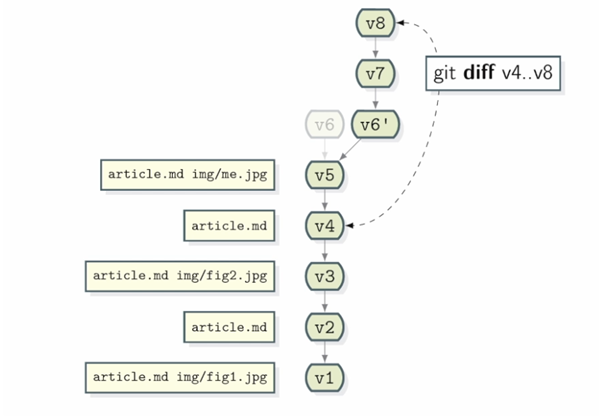
\includegraphics{./images/paste-48384992.png}

\hypertarget{import-external-data}{%
\chapter{\texorpdfstring{{📘} Import external
data}{📘 Import external data}}\label{import-external-data}}

Most of the time you will want to generate \emph{Quarto} documents using
your own data. To this aim, you will have to import data from external
sources such as files, URLs, or server data (e.g., ODK Central data).
There is a dedicated importing function in R and Python for almost every
data format. In this section we show you how to import Stata
(\texttt{.dta}), Excel (\texttt{.xlsx}) and comma-separated values (CSV,
\texttt{.csv}) data formats from files and from URLs, as well as how to
import ODK data directly from an ODK Central server.

\begin{tcolorbox}[enhanced jigsaw, colframe=quarto-callout-important-color-frame, colback=white, rightrule=.15mm, bottomrule=.15mm, left=2mm, arc=.35mm, coltitle=black, title=\textcolor{quarto-callout-important-color}{\faExclamation}\hspace{0.5em}{Important}, opacitybacktitle=0.6, bottomtitle=1mm, opacityback=0, toptitle=1mm, toprule=.15mm, colbacktitle=quarto-callout-important-color!10!white, titlerule=0mm, leftrule=.75mm, breakable]
As you import data to further process / analyse them, you have to store
the imported data in a data frame.
\end{tcolorbox}

\hypertarget{sec-import-data-from-files}{%
\section{Import data from files}\label{sec-import-data-from-files}}

All Python and R functions only require as input the path where the file
you want to import is stored. This path has to be passed as a sequence
of characters (\emph{character}) within double (``\,``) or single ('\,')
quotes.

The path can be either:

\begin{itemize}
\tightlist
\item
  relative to your Quarto document
\end{itemize}

\begin{Shaded}
\begin{Highlighting}[]
\InformationTok{\textasciigrave{}\textasciigrave{}\textasciigrave{}\{r\}}
\NormalTok{relative\_path }\OtherTok{\textless{}{-}} \StringTok{"./data/mydata.csv"}
\InformationTok{\textasciigrave{}\textasciigrave{}\textasciigrave{}}
\end{Highlighting}
\end{Shaded}

\begin{itemize}
\tightlist
\item
  absolute
\end{itemize}

\begin{Shaded}
\begin{Highlighting}[]
\InformationTok{\textasciigrave{}\textasciigrave{}\textasciigrave{}\{r\}}
\NormalTok{absolute\_path }\OtherTok{\textless{}{-}} \StringTok{"C:/Users/myuser/Documents/mydata.csv"}
\InformationTok{\textasciigrave{}\textasciigrave{}\textasciigrave{}}
\end{Highlighting}
\end{Shaded}

Functions in general have additional optional arguments.

\hypertarget{import-excel-data}{%
\subsection{Import Excel data}\label{import-excel-data}}

\hypertarget{exercise-1}{%
\subsubsection{\texorpdfstring{{✏️} Exercise
1}{✏️ Exercise 1}}\label{exercise-1}}

Import the Excel data set \textbf{dataset1.xlsx} and store it into a
data frame called \textbf{df1}.

\begin{tcolorbox}[enhanced jigsaw, colframe=quarto-callout-tip-color-frame, colback=white, rightrule=.15mm, bottomrule=.15mm, left=2mm, arc=.35mm, coltitle=black, title=\textcolor{quarto-callout-tip-color}{\faLightbulb}\hspace{0.5em}{Tip}, opacitybacktitle=0.6, bottomtitle=1mm, opacityback=0, toptitle=1mm, toprule=.15mm, colbacktitle=quarto-callout-tip-color!10!white, titlerule=0mm, leftrule=.75mm, breakable]

\begin{itemize}
\tightlist
\item
  Stata: use the
  \href{https://www.stata.com/manuals/dimportexcel.pdf}{import excel}
  Stata command with the
  \href{https://rdrr.io/github/lbraglia/RStata/man/stata.html}{stata}
  function from the \texttt{RStata} package.
\item
  R: use the
  \href{https://www.rdocumentation.org/packages/openxlsx/versions/4.2.5/topics/read.xlsx}{read.xlsx}
  function from the \texttt{openxlsx} package.
\item
  Python: use the
  \href{https://pandas.pydata.org/docs/reference/api/pandas.read_excel.html}{read\_excel}
  function from the \texttt{pandas} package.
\end{itemize}

\end{tcolorbox}

\begin{Shaded}
\begin{Highlighting}[]
\InformationTok{\textasciigrave{}\textasciigrave{}\textasciigrave{}\{r\}}
\CommentTok{\# Write your code here}
\InformationTok{\textasciigrave{}\textasciigrave{}\textasciigrave{}}
\end{Highlighting}
\end{Shaded}

\hypertarget{stata}{%
\subsubsection{Stata}\label{stata}}

Use the \href{https://www.stata.com/manuals/dimportexcel.pdf}{import
excel} Stata command with the
\href{https://rdrr.io/github/lbraglia/RStata/man/stata.html}{stata}
function from the \texttt{RStata} package.

\begin{Shaded}
\begin{Highlighting}[]
\InformationTok{\textasciigrave{}\textasciigrave{}\textasciigrave{}\{r\}}
\FunctionTok{library}\NormalTok{(RStata)}

\NormalTok{df1 }\OtherTok{\textless{}{-}}\NormalTok{ RStata}\SpecialCharTok{::}\FunctionTok{stata}\NormalTok{(}\StringTok{"import excel ./data/dataset1.xlsx"}\NormalTok{,}
                     \AttributeTok{data.out =} \ConstantTok{TRUE}\NormalTok{)}
\InformationTok{\textasciigrave{}\textasciigrave{}\textasciigrave{}}
\end{Highlighting}
\end{Shaded}

\begin{verbatim}
. import excel ./data/dataset1.xlsx
(51 vars, 10,309 obs)
\end{verbatim}

\hypertarget{r}{%
\subsubsection{R}\label{r}}

Use the
\href{https://www.rdocumentation.org/packages/openxlsx/versions/4.2.5/topics/read.xlsx}{read.xlsx}
function from the \texttt{openxlsx} package.

\begin{Shaded}
\begin{Highlighting}[]
\InformationTok{\textasciigrave{}\textasciigrave{}\textasciigrave{}\{r\}}
\FunctionTok{library}\NormalTok{(openxlsx)}

\NormalTok{df1 }\OtherTok{\textless{}{-}}\NormalTok{ openxlsx}\SpecialCharTok{::}\FunctionTok{read.xlsx}\NormalTok{(}\StringTok{"./data/dataset1.xlsx"}\NormalTok{)}
\InformationTok{\textasciigrave{}\textasciigrave{}\textasciigrave{}}
\end{Highlighting}
\end{Shaded}

\hypertarget{python}{%
\subsubsection{Python}\label{python}}

Use the
\href{https://pandas.pydata.org/docs/reference/api/pandas.read_excel.html}{read\_excel}
function from the \texttt{pandas} package.

\begin{Shaded}
\begin{Highlighting}[]
\InformationTok{\textasciigrave{}\textasciigrave{}\textasciigrave{}\{python\}}
\ImportTok{import}\NormalTok{ pandas}

\NormalTok{df1 }\OperatorTok{=}\NormalTok{ pandas.read\_excel(}\StringTok{\textquotesingle{}./data/dataset1.xlsx\textquotesingle{}}\NormalTok{)}
\InformationTok{\textasciigrave{}\textasciigrave{}\textasciigrave{}}
\end{Highlighting}
\end{Shaded}

\hypertarget{import-csv-data}{%
\subsection{Import CSV data}\label{import-csv-data}}

\hypertarget{exercise-2}{%
\subsubsection{\texorpdfstring{{✏️} Exercise
2}{✏️ Exercise 2}}\label{exercise-2}}

Read the CSV data set \textbf{dataset1.csv} and store it into a data
frame called \textbf{df2}.

\begin{tcolorbox}[enhanced jigsaw, colframe=quarto-callout-tip-color-frame, colback=white, rightrule=.15mm, bottomrule=.15mm, left=2mm, arc=.35mm, coltitle=black, title=\textcolor{quarto-callout-tip-color}{\faLightbulb}\hspace{0.5em}{Tip}, opacitybacktitle=0.6, bottomtitle=1mm, opacityback=0, toptitle=1mm, toprule=.15mm, colbacktitle=quarto-callout-tip-color!10!white, titlerule=0mm, leftrule=.75mm, breakable]

\begin{itemize}
\tightlist
\item
  Stata: use the import delimited Stata command with the
  \href{https://rdrr.io/github/lbraglia/RStata/man/stata.html}{stata}
  function from the \texttt{RStata} package.
\item
  R: use the
  \href{https://www.rdocumentation.org/packages/utils/versions/3.6.2/topics/read.table}{read.csv}
  function from the \texttt{haven} package.
\item
  Python: use the
  \href{https://pandas.pydata.org/docs/reference/api/pandas.read_csv.html}{read\_csv}
  function from the \texttt{pandas} package.
\end{itemize}

\end{tcolorbox}

\begin{Shaded}
\begin{Highlighting}[]
\InformationTok{\textasciigrave{}\textasciigrave{}\textasciigrave{}\{r\}}
\CommentTok{\# Write your code here}
\InformationTok{\textasciigrave{}\textasciigrave{}\textasciigrave{}}
\end{Highlighting}
\end{Shaded}

\hypertarget{stata-1}{%
\subsubsection{Stata}\label{stata-1}}

\begin{Shaded}
\begin{Highlighting}[]
\InformationTok{\textasciigrave{}\textasciigrave{}\textasciigrave{}\{r\}}
\CommentTok{\# library(RStata)}
\CommentTok{\# }
\CommentTok{\# df2 \textless{}{-} RStata::stata("import delimited ./data/dataset1.csv",}
\CommentTok{\#                      data.out = TRUE)}
\InformationTok{\textasciigrave{}\textasciigrave{}\textasciigrave{}}
\end{Highlighting}
\end{Shaded}

\hypertarget{r-1}{%
\subsubsection{R}\label{r-1}}

\begin{Shaded}
\begin{Highlighting}[]
\InformationTok{\textasciigrave{}\textasciigrave{}\textasciigrave{}\{r\}}
\NormalTok{df2 }\OtherTok{\textless{}{-}} \FunctionTok{read.csv}\NormalTok{(}\StringTok{"./data/dataset1.csv"}\NormalTok{)}
\InformationTok{\textasciigrave{}\textasciigrave{}\textasciigrave{}}
\end{Highlighting}
\end{Shaded}

\hypertarget{python-1}{%
\subsubsection{Python}\label{python-1}}

Use the
\href{https://pandas.pydata.org/docs/reference/api/pandas.read_csv.html}{read\_csv}
function from the \texttt{pandas} package.

\begin{Shaded}
\begin{Highlighting}[]
\InformationTok{\textasciigrave{}\textasciigrave{}\textasciigrave{}\{python\}}
\ImportTok{import}\NormalTok{ pandas}

\NormalTok{df2 }\OperatorTok{=}\NormalTok{ pandas.read\_csv(}\StringTok{\textquotesingle{}./data/dataset1.csv\textquotesingle{}}\NormalTok{)}
\InformationTok{\textasciigrave{}\textasciigrave{}\textasciigrave{}}
\end{Highlighting}
\end{Shaded}

\hypertarget{import-stata-data}{%
\subsection{Import Stata data}\label{import-stata-data}}

\hypertarget{exercise-3}{%
\subsubsection{\texorpdfstring{{✏️} Exercise
3}{✏️ Exercise 3}}\label{exercise-3}}

Read the Stata data set \textbf{dataset1.dta} and store it into a data
frame called \textbf{df3}.

\begin{tcolorbox}[enhanced jigsaw, colframe=quarto-callout-tip-color-frame, colback=white, rightrule=.15mm, bottomrule=.15mm, left=2mm, arc=.35mm, coltitle=black, title=\textcolor{quarto-callout-tip-color}{\faLightbulb}\hspace{0.5em}{Tip}, opacitybacktitle=0.6, bottomtitle=1mm, opacityback=0, toptitle=1mm, toprule=.15mm, colbacktitle=quarto-callout-tip-color!10!white, titlerule=0mm, leftrule=.75mm, breakable]

\begin{itemize}
\tightlist
\item
  Stata: use the \texttt{use} Stata command with the
  \href{https://rdrr.io/github/lbraglia/RStata/man/stata.html}{stata}
  function from the \texttt{RStata} package.
\item
  R: use the
  \href{https://haven.tidyverse.org/reference/read_dta.html}{read\_dta}
  function from the \texttt{haven} package. This package supports SAS,
  STATA and SPSS software.
\item
  Python: use the
  \href{https://pandas.pydata.org/docs/reference/api/pandas.read_stata.html}{read\_stata}
  function from the \texttt{pandas} package.
\end{itemize}

\end{tcolorbox}

\begin{Shaded}
\begin{Highlighting}[]
\InformationTok{\textasciigrave{}\textasciigrave{}\textasciigrave{}\{r\}}
\CommentTok{\# Write your code here}
\InformationTok{\textasciigrave{}\textasciigrave{}\textasciigrave{}}
\end{Highlighting}
\end{Shaded}

\hypertarget{stata-2}{%
\subsubsection{Stata}\label{stata-2}}

\begin{Shaded}
\begin{Highlighting}[]
\InformationTok{\textasciigrave{}\textasciigrave{}\textasciigrave{}\{r\}}
\FunctionTok{library}\NormalTok{(RStata)}

\NormalTok{df3 }\OtherTok{\textless{}{-}}\NormalTok{ RStata}\SpecialCharTok{::}\FunctionTok{stata}\NormalTok{(}\StringTok{"use ./data/dataset1.dta"}\NormalTok{,}
                     \AttributeTok{data.out =} \ConstantTok{TRUE}\NormalTok{)}
\InformationTok{\textasciigrave{}\textasciigrave{}\textasciigrave{}}
\end{Highlighting}
\end{Shaded}

\begin{verbatim}
. use ./data/dataset1.dta
\end{verbatim}

\hypertarget{r-2}{%
\subsubsection{R}\label{r-2}}

\begin{Shaded}
\begin{Highlighting}[]
\InformationTok{\textasciigrave{}\textasciigrave{}\textasciigrave{}\{r\}}
\FunctionTok{library}\NormalTok{(haven)}

\NormalTok{df3 }\OtherTok{\textless{}{-}}\NormalTok{ haven}\SpecialCharTok{::}\FunctionTok{read\_dta}\NormalTok{(}\StringTok{"./data/dataset1.dta"}\NormalTok{)}
\InformationTok{\textasciigrave{}\textasciigrave{}\textasciigrave{}}
\end{Highlighting}
\end{Shaded}

\hypertarget{python-2}{%
\subsubsection{Python}\label{python-2}}

Use the
\href{https://pandas.pydata.org/docs/reference/api/pandas.read_stata.html}{read\_stata}
function from the \texttt{pandas} package.

\begin{Shaded}
\begin{Highlighting}[]
\InformationTok{\textasciigrave{}\textasciigrave{}\textasciigrave{}\{python\}}
\ImportTok{import}\NormalTok{ pandas}

\NormalTok{df3 }\OperatorTok{=}\NormalTok{ pandas.read\_stata(}\StringTok{\textquotesingle{}./data/dataset1.dta\textquotesingle{}}\NormalTok{)}
\InformationTok{\textasciigrave{}\textasciigrave{}\textasciigrave{}}
\end{Highlighting}
\end{Shaded}

\hypertarget{import-data-from-urls}{%
\section{Import data from URLs}\label{import-data-from-urls}}

All functions can accept URLs as well instead of the path to a specific
file.

\hypertarget{exercise-4}{%
\subsubsection{\texorpdfstring{{✏️} Exercise
4}{✏️ Exercise 4}}\label{exercise-4}}

Import the CSV data set that contains a comprehensive spatial inventory
of 98,745 public health facilities in Sub Saharan Africa directly from
the following
\href{https://open.africa/dataset/d7335980-29d5-476c-bf7a-feb4e22cf631/resource/e2432e8a-cf15-4a8b-b8c3-567f443c1459/download/cfa-data-hospitals-in-africa-00-ssa-mfl-130219.xlsx-ssa-mfl.csv}{url}
and store it into a data frame called \textbf{df4}.

To learn more about how this data set was assembled, please refer to (5)

\begin{tcolorbox}[enhanced jigsaw, colframe=quarto-callout-tip-color-frame, colback=white, rightrule=.15mm, bottomrule=.15mm, left=2mm, arc=.35mm, coltitle=black, title=\textcolor{quarto-callout-tip-color}{\faLightbulb}\hspace{0.5em}{Tip}, opacitybacktitle=0.6, bottomtitle=1mm, opacityback=0, toptitle=1mm, toprule=.15mm, colbacktitle=quarto-callout-tip-color!10!white, titlerule=0mm, leftrule=.75mm, breakable]

\begin{itemize}
\tightlist
\item
  Stata: use the import excel Stata command with the \texttt{stata}
  function from the \texttt{RStata} package.
\item
  R: use the
  \href{https://www.rdocumentation.org/packages/openxlsx/versions/4.2.5/topics/read.xlsx}{read.xlsx}
  function from the \texttt{openxlsx} package.
\item
  Python: use the
  \href{https://pandas.pydata.org/docs/reference/api/pandas.read_excel.html}{read\_excel}
  function from the \texttt{pandas} package. In the latest version of
  pandas (0.19.2) you can directly pass the url
\end{itemize}

\end{tcolorbox}

\begin{Shaded}
\begin{Highlighting}[]
\InformationTok{\textasciigrave{}\textasciigrave{}\textasciigrave{}\{r\}}
\CommentTok{\# Write your code here}
\InformationTok{\textasciigrave{}\textasciigrave{}\textasciigrave{}}
\end{Highlighting}
\end{Shaded}

\hypertarget{stata-3}{%
\subsubsection{Stata}\label{stata-3}}

Here, because quotes are already used for the Stata command, you need to
use the other type of quotes for indicating the URL.

\begin{Shaded}
\begin{Highlighting}[]
\InformationTok{\textasciigrave{}\textasciigrave{}\textasciigrave{}\{r\}}
\FunctionTok{library}\NormalTok{(RStata)}

\NormalTok{df2 }\OtherTok{\textless{}{-}}\NormalTok{ RStata}\SpecialCharTok{::}\FunctionTok{stata}\NormalTok{(}\StringTok{\textquotesingle{}import delimited "https://open.africa/dataset/d7335980{-}29d5{-}476c{-}bf7a{-}feb4e22cf631/resource/e2432e8a{-}cf15{-}4a8b{-}b8c3{-}567f443c1459/download/cfa{-}data{-}hospitals{-}in{-}africa{-}00{-}ssa{-}mfl{-}130219.xlsx{-}ssa{-}mfl.csv"\textquotesingle{}}\NormalTok{,}
                     \AttributeTok{data.out =} \ConstantTok{TRUE}\NormalTok{)}
\InformationTok{\textasciigrave{}\textasciigrave{}\textasciigrave{}}
\end{Highlighting}
\end{Shaded}

\begin{verbatim}
. import delimited "https://open.africa/dataset/d7335980-29d5-476c-bf7a-feb4e22
> cf631/resource/e2432e8a-cf15-4a8b-b8c3-567f443c1459/download/cfa-data-hospita
> ls-in-africa-00-ssa-mfl-130219.xlsx-ssa-mfl.csv"
(7 vars, 98,745 obs)
\end{verbatim}

\hypertarget{r-3}{%
\subsubsection{R}\label{r-3}}

Use the
\href{https://www.rdocumentation.org/packages/openxlsx/versions/4.2.5/topics/read.xlsx}{read.xlsx}
function from the \texttt{openxlsx} package.

\begin{Shaded}
\begin{Highlighting}[]
\InformationTok{\textasciigrave{}\textasciigrave{}\textasciigrave{}\{r\}}
\NormalTok{csv\_url }\OtherTok{\textless{}{-}} \StringTok{"https://open.africa/dataset/d7335980{-}29d5{-}476c{-}bf7a{-}feb4e22cf631/resource/e2432e8a{-}cf15{-}4a8b{-}b8c3{-}567f443c1459/download/cfa{-}data{-}hospitals{-}in{-}africa{-}00{-}ssa{-}mfl{-}130219.xlsx{-}ssa{-}mfl.csv"}
\NormalTok{df4 }\OtherTok{\textless{}{-}} \FunctionTok{read.csv}\NormalTok{(csv\_url)}
\InformationTok{\textasciigrave{}\textasciigrave{}\textasciigrave{}}
\end{Highlighting}
\end{Shaded}

\hypertarget{python-3}{%
\subsubsection{Python}\label{python-3}}

Use the
\href{https://pandas.pydata.org/docs/reference/api/pandas.read_excel.html}{read\_excel}
function from the \texttt{pandas} package.

\begin{Shaded}
\begin{Highlighting}[]
\InformationTok{\textasciigrave{}\textasciigrave{}\textasciigrave{}\{python\}}
\ImportTok{import}\NormalTok{ pandas}

\NormalTok{csv\_url }\OperatorTok{=} \StringTok{"https://open.africa/dataset/d7335980{-}29d5{-}476c{-}bf7a{-}feb4e22cf631/resource/e2432e8a{-}cf15{-}4a8b{-}b8c3{-}567f443c1459/download/cfa{-}data{-}hospitals{-}in{-}africa{-}00{-}ssa{-}mfl{-}130219.xlsx{-}ssa{-}mfl.csv"}
\NormalTok{df1 }\OperatorTok{=}\NormalTok{ pandas.read\_csv(csv\_url)}
\InformationTok{\textasciigrave{}\textasciigrave{}\textasciigrave{}}
\end{Highlighting}
\end{Shaded}

\hypertarget{manipulate-data}{%
\chapter{\texorpdfstring{{📘} Manipulate
data}{📘 Manipulate data}}\label{manipulate-data}}

\begin{tcolorbox}[enhanced jigsaw, colframe=quarto-callout-important-color-frame, colback=white, rightrule=.15mm, bottomrule=.15mm, left=2mm, arc=.35mm, coltitle=black, title=\textcolor{quarto-callout-important-color}{\faExclamation}\hspace{0.5em}{Important}, opacitybacktitle=0.6, bottomtitle=1mm, opacityback=0, toptitle=1mm, toprule=.15mm, colbacktitle=quarto-callout-important-color!10!white, titlerule=0mm, leftrule=.75mm, breakable]
Remember that with Quarto you can store multiple data sets in memory
(stored in different data frames \texttt{df1}, \texttt{df2},
\texttt{df3}, etc) and work in parallel on all these data sets.
\end{tcolorbox}

\hypertarget{type-of-data}{%
\section{Type of data}\label{type-of-data}}

\hypertarget{descriptive-statistics}{%
\section{Descriptive statistics}\label{descriptive-statistics}}

\hypertarget{visualise-data}{%
\section{Visualise data}\label{visualise-data}}

\hypertarget{manipulate-python-and-r-data}{%
\section{Manipulate Python and R
data}\label{manipulate-python-and-r-data}}

\hypertarget{exercise-1-1}{%
\subsubsection{\texorpdfstring{{✏️} Exercise
1}{✏️ Exercise 1}}\label{exercise-1-1}}

\begin{enumerate}
\def\labelenumi{\arabic{enumi}.}
\tightlist
\item
  Import \textbf{dataset1.xlsx} using Stata and store it in \texttt{df1}
\end{enumerate}

\begin{Shaded}
\begin{Highlighting}[]
\InformationTok{\textasciigrave{}\textasciigrave{}\textasciigrave{}\{r\}}
\CommentTok{\# Write your code here}
\InformationTok{\textasciigrave{}\textasciigrave{}\textasciigrave{}}
\end{Highlighting}
\end{Shaded}

\begin{enumerate}
\def\labelenumi{\arabic{enumi}.}
\setcounter{enumi}{1}
\tightlist
\item
  Import \textbf{dataset1.csv} using Python and store it in \texttt{df2}
\end{enumerate}

\begin{Shaded}
\begin{Highlighting}[]
\InformationTok{\textasciigrave{}\textasciigrave{}\textasciigrave{}\{python\}}
\CommentTok{\# Write your code here}
\InformationTok{\textasciigrave{}\textasciigrave{}\textasciigrave{}}
\end{Highlighting}
\end{Shaded}

\begin{enumerate}
\def\labelenumi{\arabic{enumi}.}
\setcounter{enumi}{2}
\tightlist
\item
  Compare \texttt{df1}and \texttt{df2}. Can you indicate what variable
  has been modified in \textbf{dataset1} between df1 and df2?
\end{enumerate}

\begin{tcolorbox}[enhanced jigsaw, colframe=quarto-callout-tip-color-frame, colback=white, rightrule=.15mm, bottomrule=.15mm, left=2mm, arc=.35mm, coltitle=black, title=\textcolor{quarto-callout-tip-color}{\faLightbulb}\hspace{0.5em}{Tip}, opacitybacktitle=0.6, bottomtitle=1mm, opacityback=0, toptitle=1mm, toprule=.15mm, colbacktitle=quarto-callout-tip-color!10!white, titlerule=0mm, leftrule=.75mm, breakable]
Use the R function \textbf{comparedf}
\end{tcolorbox}

\begin{Shaded}
\begin{Highlighting}[]
\InformationTok{\textasciigrave{}\textasciigrave{}\textasciigrave{}\{r\}}
\CommentTok{\# Write your code here}
\InformationTok{\textasciigrave{}\textasciigrave{}\textasciigrave{}}
\end{Highlighting}
\end{Shaded}

\hypertarget{solution}{%
\subsubsection{\texorpdfstring{{👀}
Solution}{👀 Solution}}\label{solution}}

\begin{enumerate}
\def\labelenumi{\arabic{enumi}.}
\tightlist
\item
  Import \textbf{dataset1.xlsx} using Stata and store it in \texttt{df1}
\end{enumerate}

\begin{Shaded}
\begin{Highlighting}[]
\InformationTok{\textasciigrave{}\textasciigrave{}\textasciigrave{}\{r\}}
\FunctionTok{library}\NormalTok{(RStata)}
\NormalTok{df1 }\OtherTok{\textless{}{-}}\NormalTok{ RStata}\SpecialCharTok{::}\FunctionTok{stata}\NormalTok{(}\StringTok{"import excel ./data/dataset1.xlsx"}\NormalTok{,}
                     \AttributeTok{data.out =} \ConstantTok{TRUE}\NormalTok{)}
\InformationTok{\textasciigrave{}\textasciigrave{}\textasciigrave{}}
\end{Highlighting}
\end{Shaded}

\begin{verbatim}
. import excel ./data/dataset1.xlsx
(51 vars, 10,309 obs)
\end{verbatim}

\begin{enumerate}
\def\labelenumi{\arabic{enumi}.}
\setcounter{enumi}{1}
\tightlist
\item
  Import \textbf{dataset1.csv} using Python and store it in \texttt{df2}
\end{enumerate}

\begin{Shaded}
\begin{Highlighting}[]
\InformationTok{\textasciigrave{}\textasciigrave{}\textasciigrave{}\{python\}}
\ImportTok{import}\NormalTok{ pandas }\ImportTok{as}\NormalTok{ pd}
\NormalTok{df2 }\OperatorTok{=}\NormalTok{ pd.read\_csv(}\StringTok{\textquotesingle{}./data/dataset1.csv\textquotesingle{}}\NormalTok{)}
\InformationTok{\textasciigrave{}\textasciigrave{}\textasciigrave{}}
\end{Highlighting}
\end{Shaded}

\begin{enumerate}
\def\labelenumi{\arabic{enumi}.}
\setcounter{enumi}{2}
\tightlist
\item
  Compare \texttt{df1}and \texttt{df2}.
\end{enumerate}

\begin{Shaded}
\begin{Highlighting}[]
\InformationTok{\textasciigrave{}\textasciigrave{}\textasciigrave{}\{r\}}
\FunctionTok{library}\NormalTok{(reticulate)}
\InformationTok{\textasciigrave{}\textasciigrave{}\textasciigrave{}}
\end{Highlighting}
\end{Shaded}

\begin{verbatim}
Warning: Paket 'reticulate' wurde unter R Version 4.1.3 erstellt
\end{verbatim}

\begin{Shaded}
\begin{Highlighting}[]
\InformationTok{\textasciigrave{}\textasciigrave{}\textasciigrave{}\{r\}}
\NormalTok{arsenal}\SpecialCharTok{::}\FunctionTok{comparedf}\NormalTok{(df1, py}\SpecialCharTok{$}\NormalTok{df2)}
\InformationTok{\textasciigrave{}\textasciigrave{}\textasciigrave{}}
\end{Highlighting}
\end{Shaded}

\begin{verbatim}
Compare Object

Function Call: 
arsenal::comparedf(x = df1, y = py$df2)

Shared: 0 non-by variables and 10308 observations.
Not shared: 102 variables and 1 observations.

Differences found in 0/0 variables compared.
0 variables compared have non-identical attributes.
\end{verbatim}

\hypertarget{share-code-and-collaborate-with-git}{%
\chapter{\texorpdfstring{{📘} Share code and collaborate with
Git}{📘 Share code and collaborate with Git}}\label{share-code-and-collaborate-with-git}}

\hypertarget{overview-5}{%
\subsection{Overview}\label{overview-5}}

\hypertarget{learning-objectives-6}{%
\subsection{Learning objectives}\label{learning-objectives-6}}

\hypertarget{sharing-your-code-with-git}{%
\section{Sharing your code with Git}\label{sharing-your-code-with-git}}

Even if we do not take advantage of the advanced and powerful version
control functionality, we can still use Git and GitHub to share our
code.

\hypertarget{access-a-remote-github-repository}{%
\section{Access a remote GitHub
repository}\label{access-a-remote-github-repository}}

\hypertarget{collaborating-with-git}{%
\section{Collaborating with Git}\label{collaborating-with-git}}

Once you set up a central repository, you can have multiple people make
changes to code and keep versions synced. GitHub provides a free service
for centralized repositories. GitHub also has a special utility, called
a pull request, that can be used by anybody to suggest changes to your
code. You can easily either accept or deny the request.

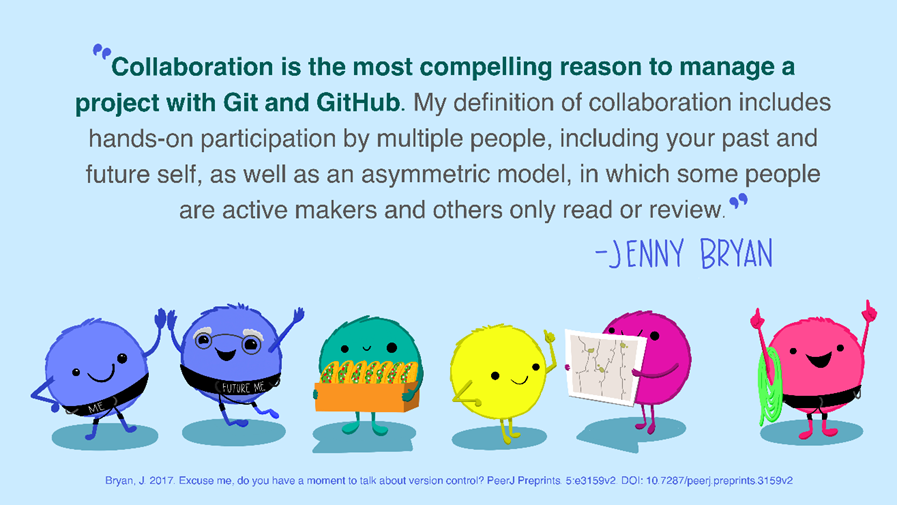
\includegraphics{./images/paste-ADC9719C.png}

\part{------------ DAY 2 ------------}

\hypertarget{data-science-for-public-health}{%
\chapter{\texorpdfstring{{📚} Data Science for Public
Health}{📚 Data Science for Public Health}}\label{data-science-for-public-health}}

\hypertarget{data-science}{%
\section{Data Science}\label{data-science}}

\hypertarget{activity-1}{%
\subsubsection{\texorpdfstring{Activity 1
{❓}}{Activity 1 ❓}}\label{activity-1}}

{🕒} 3 minutes: You have probably already heard about data science as
this is a main Data Science is today one of the main buzzwords, but what
does \textbf{Data Science} mean for you?

\hypertarget{quote-1}{%
\subsubsection{\texorpdfstring{Quote 1
{💬}}{Quote 1 💬}}\label{quote-1}}

The statistics profession faces a choice in its future research between
continuing concentration on traditional topics -- based largely on data
analysis supported by mathematical statistics -- and a broader viewpoint
-- based on an inclusive concept of \textbf{learning from data}. The
latter course present severe challenges as well as exciting
opportunities. The former risks seeing statistics become increasingly
marginal\ldots{} (6)

\textbf{John Chambers} (PhD in Statistics) is the creator of the S
programming language, and a core member of the R programming language
project.

\hypertarget{quote-2}{%
\subsubsection{\texorpdfstring{Quote 2
{💬}}{Quote 2 💬}}\label{quote-2}}

Data science is the science of \textbf{learning from data}; it studies
the methods involved in the analysis and processing of data and proposes
technology to \textbf{improve methods in an evidence-based manner}. The
scope and impact of this science will expand enormously in coming
decades as scientific data and data about science itself become
ubiquitously available. (7).

\textbf{David Donoho} is a Professor of Statistics at Stanford
University.

\hypertarget{quote-1-1}{%
\subsubsection{Quote 1}\label{quote-1-1}}

\begin{itemize}
\tightlist
\item
  Growing field with computational power and data generation
\item
  Set of collective evidence-based processes, theories, concepts, tools
  and technologies
\item
  Extraction of valuable knowledge and information from data (learning
  from data)
\end{itemize}

Qualitative thinking currently does not receive nearly as much attention
as quantitative thinking in data science.

\hypertarget{discussion-2}{%
\subsubsection{\texorpdfstring{Discussion
{💬}}{Discussion 💬}}\label{discussion-2}}

What does Data Science mean for you?

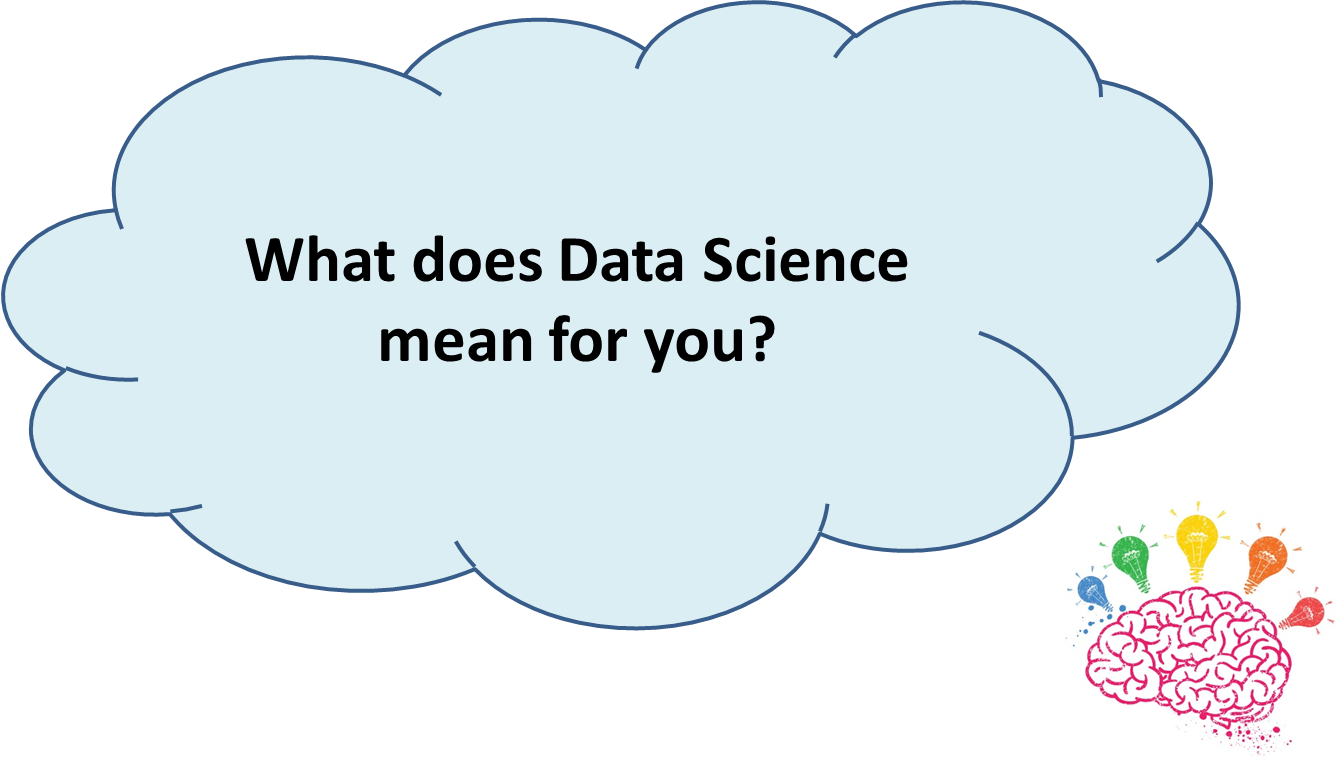
\includegraphics{./images/paste-AC41DECB.png}

\hypertarget{from-literature}{%
\subsubsection{From literature}\label{from-literature}}

Had you thought of any of those words? Word cloud generated by
\href{https://monkeylearn.com/word-cloud/}{MonkeyLearn} from (8)

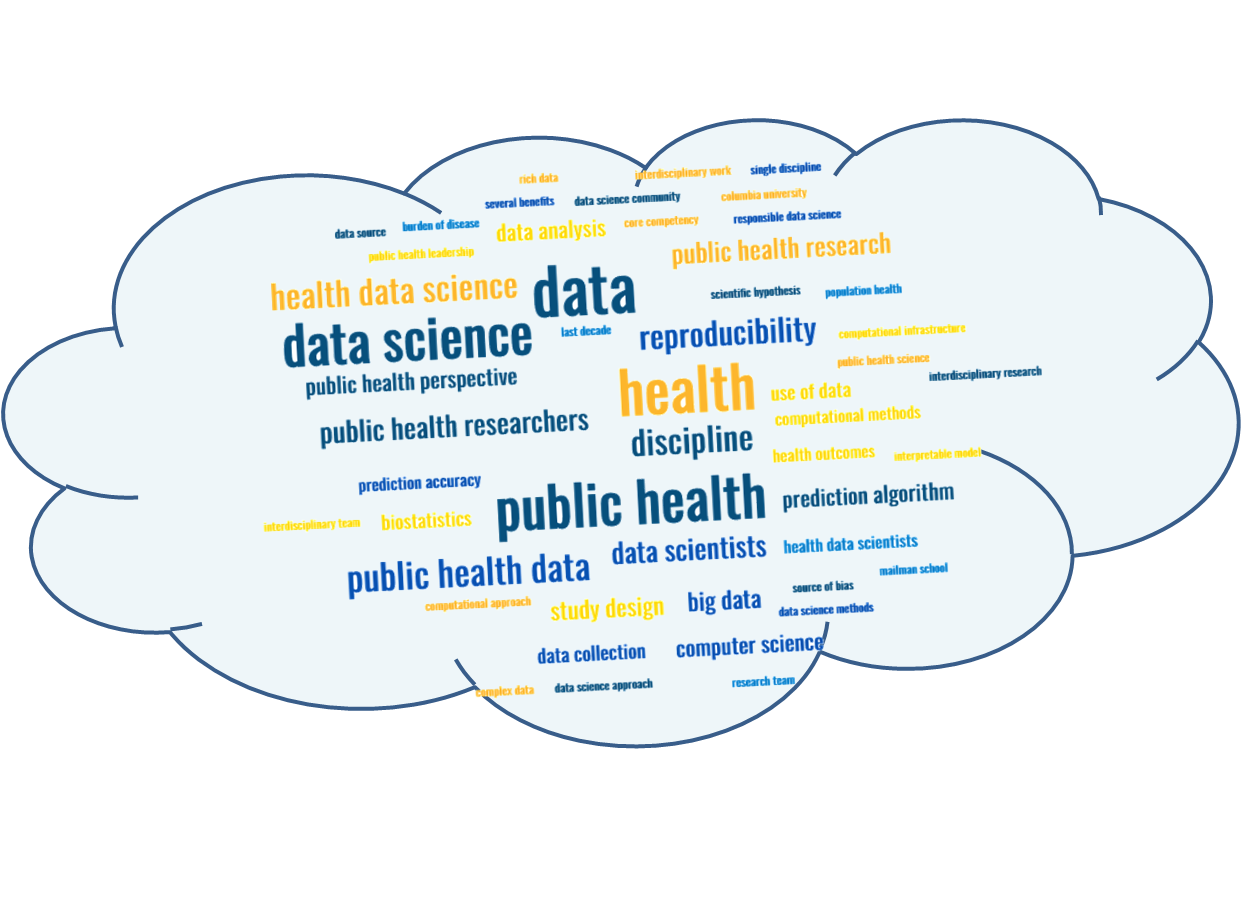
\includegraphics{./images/paste-FFA998D0.png}

\hypertarget{where-do-you-see-yourself-on-this-venn-diagram}{%
\subsection{Where do you see yourself on this Venn
diagram}\label{where-do-you-see-yourself-on-this-venn-diagram}}

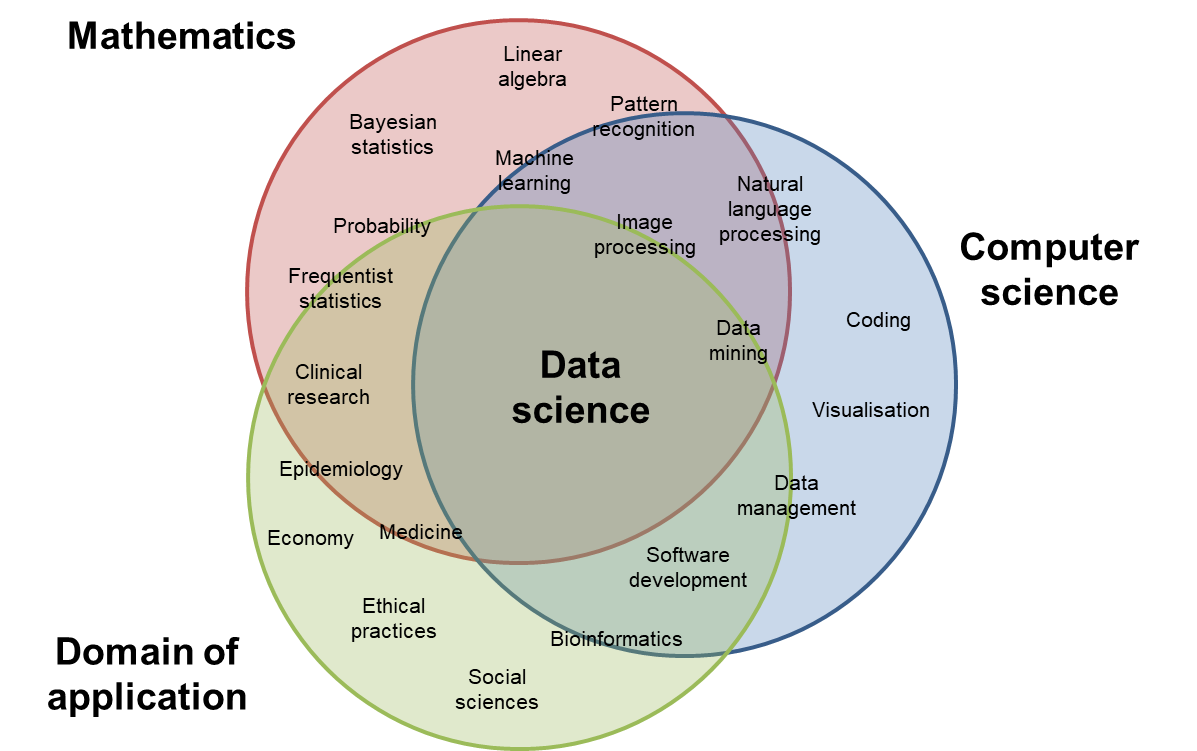
\includegraphics{./images/paste-494B1CA8.png}

\hypertarget{what-do-experts-say-about-data-science}{%
\section{What do experts say about Data
Science?}\label{what-do-experts-say-about-data-science}}

The statistics profession faces a choice in its future research between
continuing concentration on traditional topics -- based largely on data
analysis supported by mathematical statistics -- and a broader viewpoint
-- based on an inclusive concept of learning from data. The latter
course present severe challenges as well as exciting opportunities. The
former risks seeing statistics become increasingly marginal\ldots{} John
Chambers\footnote{John Chambers is a PhD in Statistics, the creator of
  the S programming language, and a core member of the R programming
  language project.} (6)

``Data science is the science of learning from data; it studies the
methods involved in the analysis and processing of data and proposes
technology to improve methods in an evidence-based manner. The scope and
impact of this science will expand enormously in coming decades as
scientific data and data about science itself become ubiquitously
available. David Donoho\footnote{David Donoho is a Professor of
  Statistics at Stanford University.} (7).

Public health data science is the study of formulating and rigorously
answering questions in order to advance health and well-being using a
data-centric process that emphasizes clarity, reproducibility, effective
communication, and ethical practices. {[}\ldots{]} Data science implies
a perspective that is shaped by {[}\ldots{]} interdisciplinary work.
Goldsmith J, Sun Y, Fried LP, Wing J, Miller GW and Berhane K (2021) The
Emergence and Future of Public Health Data Science. Public Health Rev
42:1604023.

\hypertarget{a-tentative-definition}{%
\section{A tentative definition}\label{a-tentative-definition}}

NIH defines data science as ``the interdisciplinary field of inquiry in
which quantitative and analytical approaches, processes, and systems are
developed and used to extract knowledge and insights from increasingly
large and/or complex sets of data''

In this book, we define data science as

Data science is an interdisciplinary collaborative field that tries to
answer rigorously formulated public health questions by relying on a set
of collective evidence-based processes, theories, concepts, tools and
technologies that enable the extraction of valuable knowledge and
information from data to generate actionable insights that effectively
communicated to decision-makers can advance health and well-being.

\begin{itemize}
\tightlist
\item
  Interdisciplinary collaborative field
\item
  Rigorous public health question formulation
\item
  Set of collective evidence-based processes, theories, concepts, tools
  and technologies
\item
  Extraction of valuable knowledge and information from data
\item
  Generation of actionable insights
\item
  Effective communication to decision-makers
\end{itemize}

\hypertarget{malaria-case-study}{%
\chapter{\texorpdfstring{{📚} Malaria case
study}{📚 Malaria case study}}\label{malaria-case-study}}

\hypertarget{overview-6}{%
\subsection{Overview}\label{overview-6}}

These pages will demonstrate how to use Quarto to data from Tanzania.

\hypertarget{learning-objectives-7}{%
\subsection{Learning objectives}\label{learning-objectives-7}}

\begin{itemize}
\tightlist
\item
  Apply what you have learnt on Day 1 on real data
\end{itemize}

\hypertarget{getting-started}{%
\section{Getting started}\label{getting-started}}

\hypertarget{access-the-quarto-template}{%
\subsection{Access the Quarto
template}\label{access-the-quarto-template}}

Download the Quarto template used for this case study (add link) using
GitHub.

Please review previous sections on Quarto, data import and manipulation.

\hypertarget{install-packages}{%
\subsection{Install packages}\label{install-packages}}

\begin{Shaded}
\begin{Highlighting}[]
\InformationTok{\textasciigrave{}\textasciigrave{}\textasciigrave{}\{r\}}
\FunctionTok{install.packages}\NormalTok{(}\StringTok{"ggplot2"}\NormalTok{)}
\FunctionTok{install.packages}\NormalTok{(}\StringTok{"ggthemes"}\NormalTok{)}
\FunctionTok{install.packages}\NormalTok{(}\StringTok{"networkD3"}\NormalTok{)}
\FunctionTok{install.packages}\NormalTok{(}\StringTok{"apyramid"}\NormalTok{)}
\InformationTok{\textasciigrave{}\textasciigrave{}\textasciigrave{}}
\end{Highlighting}
\end{Shaded}

\begin{Shaded}
\begin{Highlighting}[]
\InformationTok{\textasciigrave{}\textasciigrave{}\textasciigrave{}\{r\}}
\FunctionTok{library}\NormalTok{(openxlsx)}
\FunctionTok{library}\NormalTok{(dplyr)}
\FunctionTok{library}\NormalTok{(skimr)}
\FunctionTok{library}\NormalTok{(gtsummary)}
\FunctionTok{library}\NormalTok{(finalfit)}
\FunctionTok{library}\NormalTok{(ggplot2)}
\FunctionTok{library}\NormalTok{(ggthemes)}
\FunctionTok{library}\NormalTok{(networkD3) }\CommentTok{\# For alluvial/Sankey diagrams}
\FunctionTok{library}\NormalTok{(tidyverse)}
\InformationTok{\textasciigrave{}\textasciigrave{}\textasciigrave{}}
\end{Highlighting}
\end{Shaded}

\hypertarget{dataset-description}{%
\subsection{Dataset description}\label{dataset-description}}

We will be using data and examples from a real consultation data which
occurred in Tanzania between \textbf{2021-07-29} and \textbf{2021-12-17}
within the Integrated Management of Childhood Illness (TIMCI) project.

\begin{tcolorbox}[enhanced jigsaw, colframe=quarto-callout-important-color-frame, colback=white, rightrule=.15mm, bottomrule=.15mm, left=2mm, arc=.35mm, coltitle=black, title=\textcolor{quarto-callout-important-color}{\faExclamation}\hspace{0.5em}{Important}, opacitybacktitle=0.6, bottomtitle=1mm, opacityback=0, toptitle=1mm, toprule=.15mm, colbacktitle=quarto-callout-important-color!10!white, titlerule=0mm, leftrule=.75mm, breakable]
Data are made available by the Ifakara Health Institute (IHI) for
training purposes only. Please note, that some data has been adapted in
order to best achieve training objectives. No personally indentifiable
information have been kept in this dataset.
\end{tcolorbox}

Information about the consultations of \textbf{10,308 children {[}1 day
- 59 months{]}} from \textbf{18 facilities} (dispensaries and health
centres) in \textbf{Kaliua} District, \textbf{Sengerema} District and
\textbf{Tanga} District, Tanzania.

\begin{figure}

\begin{minipage}[t]{0.50\linewidth}

{\centering 

\raisebox{-\height}{

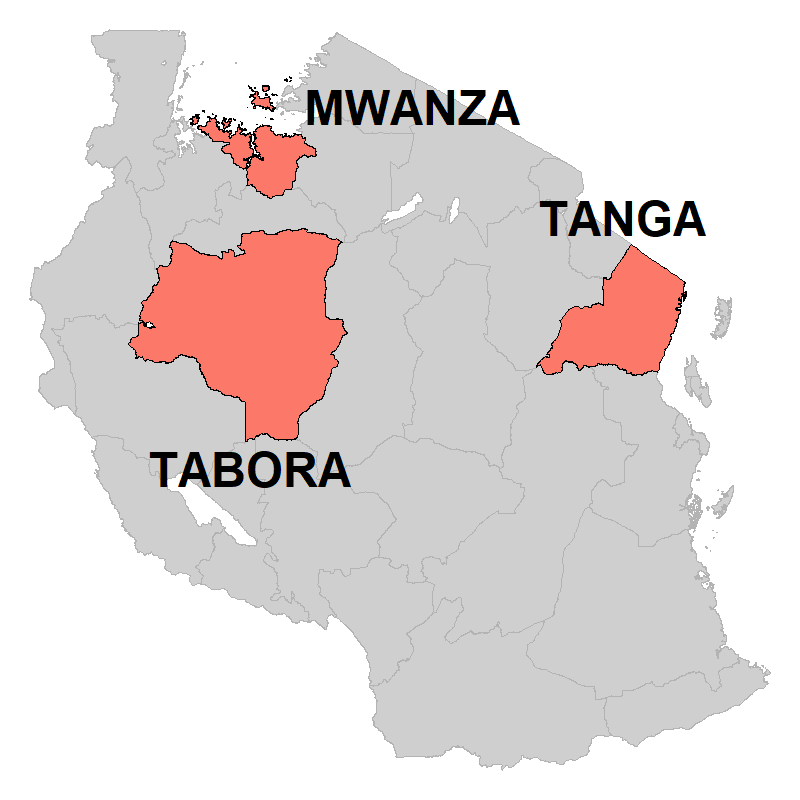
\includegraphics{./images/tanzania_map-01.png}

}

}

\subcaption{\label{fig-tanzania-study-regions}}
\end{minipage}%
%
\begin{minipage}[t]{0.50\linewidth}

{\centering 

\raisebox{-\height}{

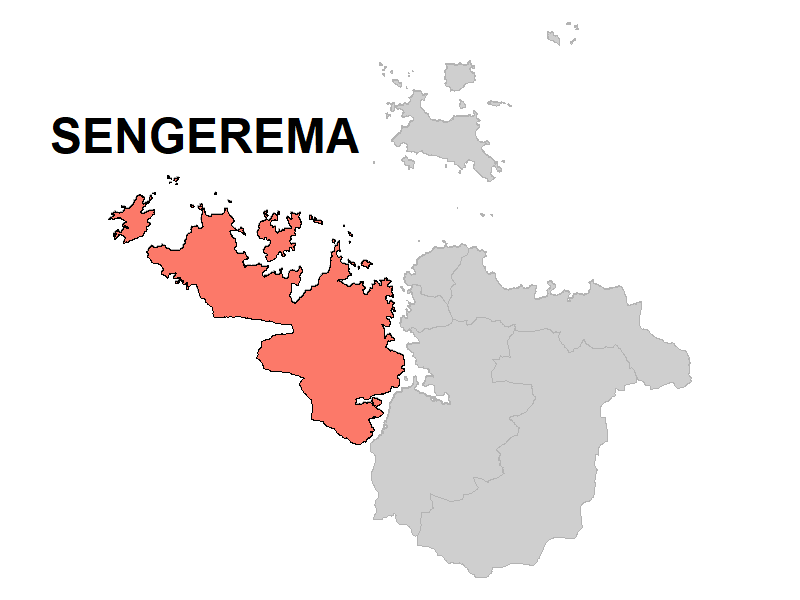
\includegraphics{./images/mwanza_map.png}

}

}

\subcaption{\label{fig-mwanza-study-district}}
\end{minipage}%
\newline
\begin{minipage}[t]{0.50\linewidth}

{\centering 

\raisebox{-\height}{


\includegraphics{./images/kaliua_map.png}

}

}

\subcaption{\label{fig-kaliua-study-district}}
\end{minipage}%
%
\begin{minipage}[t]{0.50\linewidth}

{\centering 

\raisebox{-\height}{

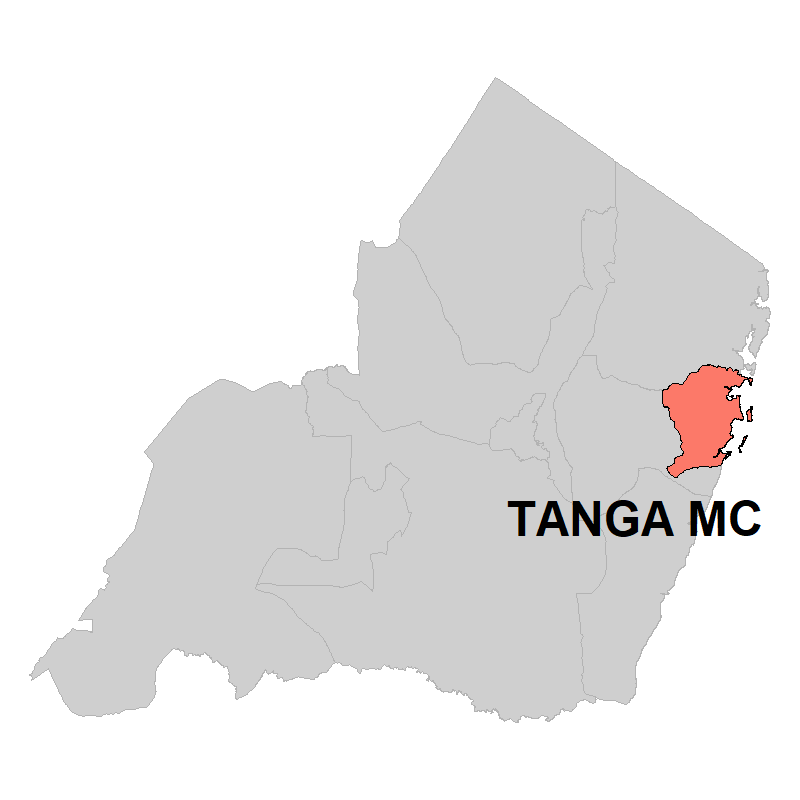
\includegraphics{./images/tanga_map.png}

}

}

\subcaption{\label{fig-tanga-study-district}}
\end{minipage}%

\caption{\label{fig-study-area}Study area}

\end{figure}

\hypertarget{data-collection}{%
\subsection{Data collection}\label{data-collection}}

Data were collected using \emph{ODK} (ODK Collect, ODK Central) between
\textbf{2021-07-29} and \textbf{2021-12-17}. Research assistants
recorded the following information from different sources.

\begin{longtable}[]{@{}
  >{\raggedright\arraybackslash}p{(\columnwidth - 4\tabcolsep) * \real{0.4130}}
  >{\centering\arraybackslash}p{(\columnwidth - 4\tabcolsep) * \real{0.1522}}
  >{\centering\arraybackslash}p{(\columnwidth - 4\tabcolsep) * \real{0.4239}}@{}}
\caption{Types and sources of information}\tabularnewline
\toprule()
\begin{minipage}[b]{\linewidth}\raggedright
Information
\end{minipage} & \begin{minipage}[b]{\linewidth}\centering
Prefix
\end{minipage} & \begin{minipage}[b]{\linewidth}\centering
Source
\end{minipage} \\
\midrule()
\endfirsthead
\toprule()
\begin{minipage}[b]{\linewidth}\raggedright
Information
\end{minipage} & \begin{minipage}[b]{\linewidth}\centering
Prefix
\end{minipage} & \begin{minipage}[b]{\linewidth}\centering
Source
\end{minipage} \\
\midrule()
\endhead
Context & CTX & Metadata \\
Sociodemographics & SDC & Caregiver \\
Clinical presentation & CLIN & Caregiver \\
Laboratory investigations & TEST & Child booklet or facility MTUHA
book \\
Diagnoses & DX & Child booklet or facility MTUHA book \\
Treatments & RX & \\
\begin{minipage}[t]{\linewidth}\raggedright
\begin{itemize}
\tightlist
\item
  before consultation
\end{itemize}
\end{minipage} & & Caregiver \\
\begin{minipage}[t]{\linewidth}\raggedright
\begin{itemize}
\tightlist
\item
  as a result of the consultation
\end{itemize}
\end{minipage} & & Child booklet or facility MTUHA book \\
Referral advice & MGMT & \\
& & Caregiver \\
& & Child booklet or facility MTUHA book \\
\bottomrule()
\end{longtable}

\hypertarget{data-preparation}{%
\subsection{Data preparation}\label{data-preparation}}

Data cleaning and data de-identification

Personally identifiable information (PII) were removed.

\hypertarget{population-characteristics}{%
\section{Population characteristics}\label{population-characteristics}}

\hypertarget{codebook}{%
\subsection{Codebook}\label{codebook}}

\begin{longtable}[]{@{}
  >{\raggedright\arraybackslash}p{(\columnwidth - 2\tabcolsep) * \real{0.4167}}
  >{\raggedright\arraybackslash}p{(\columnwidth - 2\tabcolsep) * \real{0.2222}}@{}}
\toprule()
\begin{minipage}[b]{\linewidth}\raggedright
Variable
\end{minipage} & \begin{minipage}[b]{\linewidth}\raggedright
Coding
\end{minipage} \\
\midrule()
\endhead
SDC\_age\_in\_month & \\
SDC\_sex & \begin{minipage}[t]{\linewidth}\raggedright
1: male\\
2: female\\
98: unknown\strut
\end{minipage} \\
CLIN\_fever & \begin{minipage}[t]{\linewidth}\raggedright
0: no\\
1: yes\\
98: not sure\strut
\end{minipage} \\
CLIN\_fever\_onset & \\
CLIN\_cough & \begin{minipage}[t]{\linewidth}\raggedright
0: no\\
1: yes\\
98: not sure\strut
\end{minipage} \\
CLIN\_diarrhoea & \begin{minipage}[t]{\linewidth}\raggedright
0: no\\
1: yes\\
98: not sure\strut
\end{minipage} \\
RX\_preconsult\_antibiotics & \\
RX\_preconsult\_antimalarials & \\
CONSULT\_district & \begin{minipage}[t]{\linewidth}\raggedright
Kaliua\\
Sengerema\\
Tanga\strut
\end{minipage} \\
CONSULT\_area & \begin{minipage}[t]{\linewidth}\raggedright
urban\\
rural\strut
\end{minipage} \\
CONSULT\_facility\_type & \begin{minipage}[t]{\linewidth}\raggedright
dispensary\\
health centre\strut
\end{minipage} \\
\bottomrule()
\end{longtable}

\part{------------ DAY 3 ------------}

\hypertarget{big-data-and-machine-learning}{%
\chapter{\texorpdfstring{{📚} Big data and machine
learning}{📚 Big data and machine learning}}\label{big-data-and-machine-learning}}

\hypertarget{overview-7}{%
\subsection{Overview}\label{overview-7}}

\hypertarget{learning-objectives-8}{%
\subsection{Learning objectives}\label{learning-objectives-8}}

\begin{itemize}
\item
  key dates and vcabular from the Artificial Intelligence community
\item
  machine learning vs.~statistics
\item
  trade-off between accuracy and generalisability
\end{itemize}

\hypertarget{development-of-artificial-intelligence}{%
\section{Development of Artificial
Intelligence}\label{development-of-artificial-intelligence}}

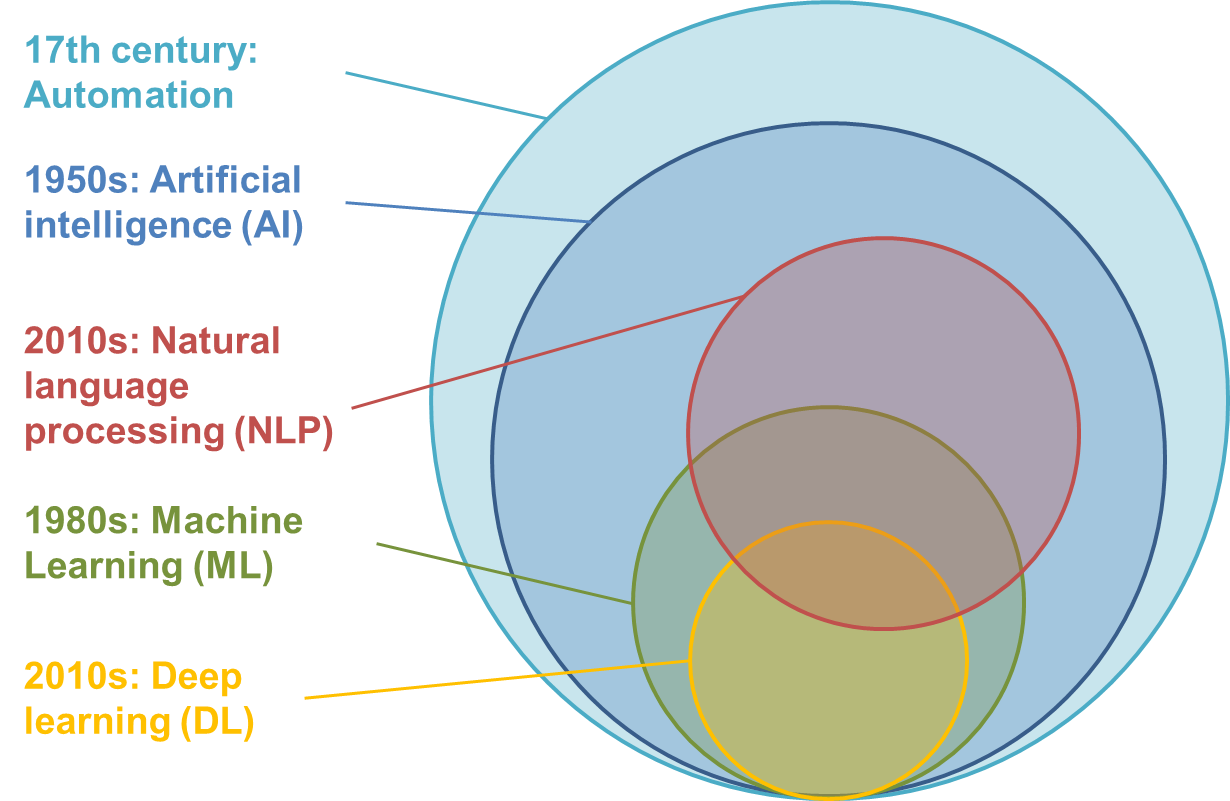
\includegraphics{./images/paste-FA238456.png}

\hypertarget{machine-learning-vs.-statistics}{%
\section{Machine Learning
vs.~Statistics}\label{machine-learning-vs.-statistics}}

\hypertarget{inference}{%
\subsubsection{Inference}\label{inference}}

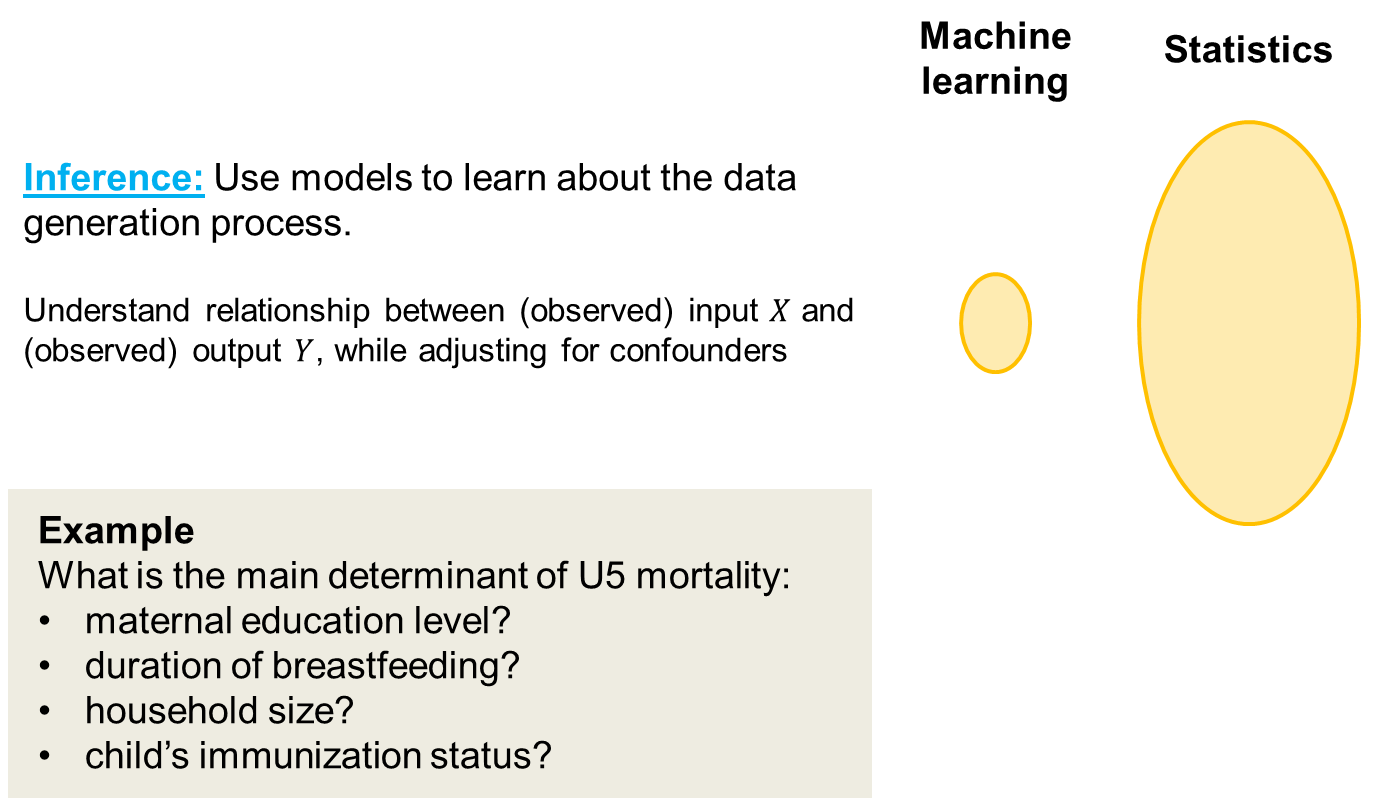
\includegraphics{./images/paste-C70B4C10.png}

\hypertarget{prediction}{%
\subsubsection{Prediction}\label{prediction}}

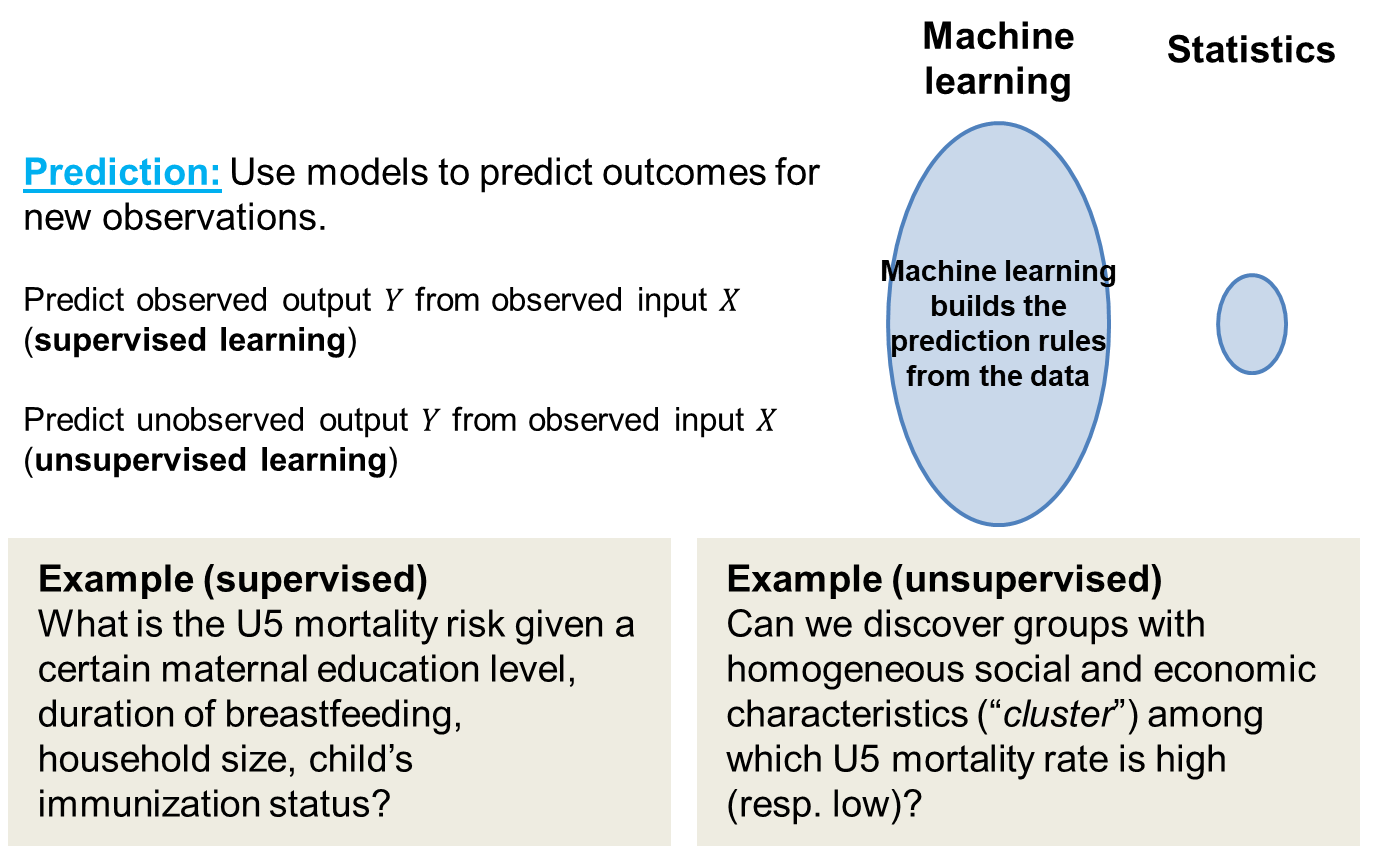
\includegraphics{./images/paste-2C4E6936.png}

\hypertarget{learning-from-data-accuracy-or-generalizability}{%
\section{Learning From Data: Accuracy or
Generalizability?}\label{learning-from-data-accuracy-or-generalizability}}

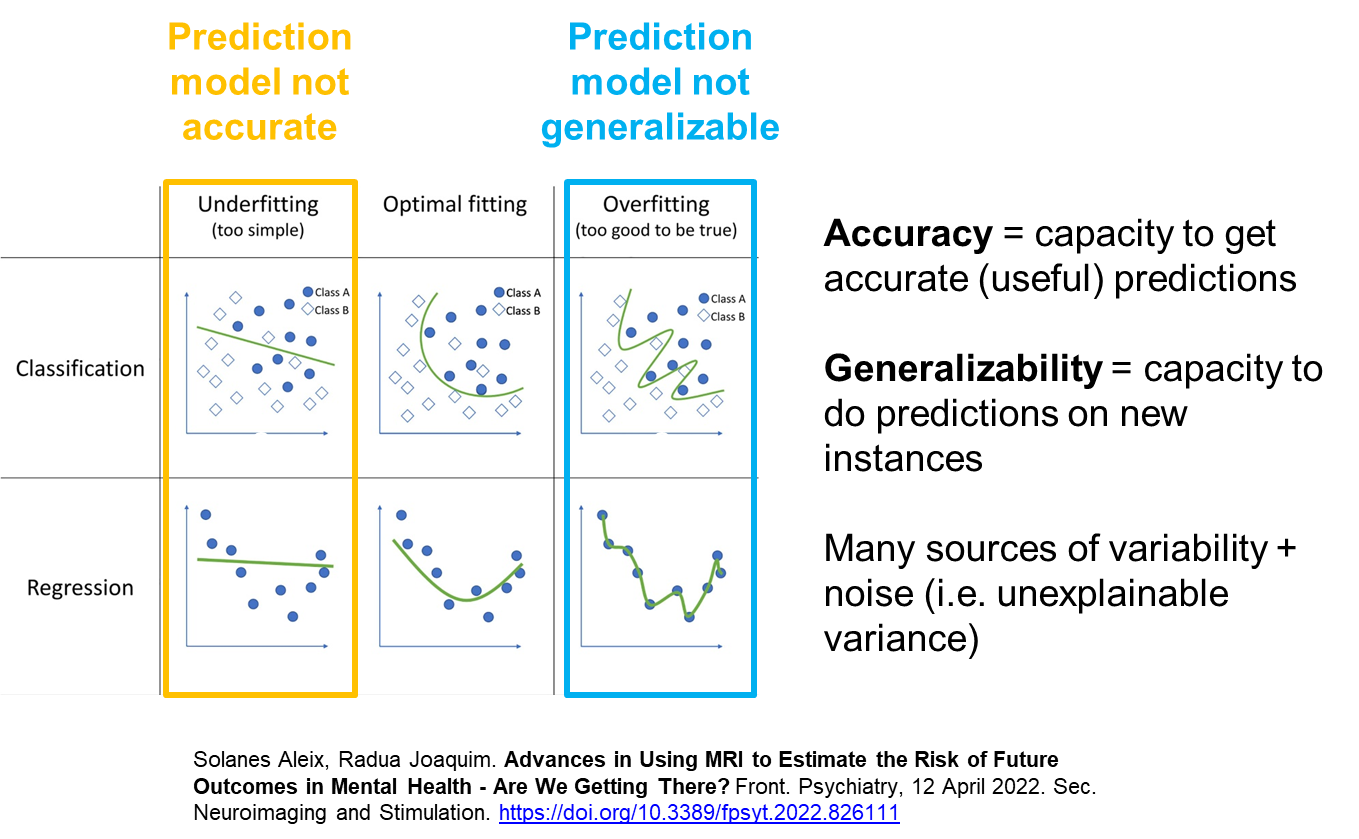
\includegraphics{./images/paste-FC3A1160.png}

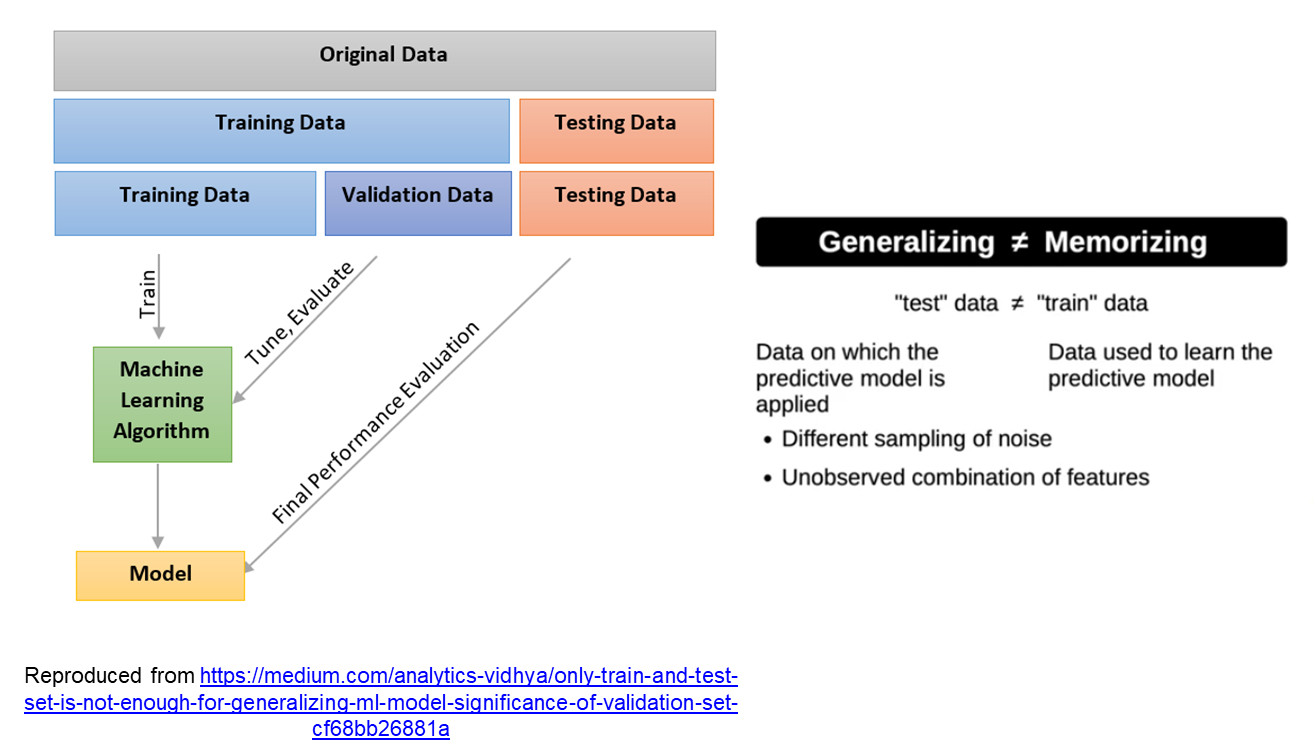
\includegraphics{./images/paste-7D73149D.png}

\bookmarksetup{startatroot}

\hypertarget{references-2}{%
\chapter*{References}\label{references-2}}
\addcontentsline{toc}{chapter}{References}

\hypertarget{refs}{}
\begin{CSLReferences}{0}{0}
\leavevmode\vadjust pre{\hypertarget{ref-the_turing_way_community_2022_6909298}{}}%
\CSLLeftMargin{1. }%
\CSLRightInline{The Turing Way Community. {The Turing Way: A handbook
for reproducible, ethical and collaborative research} {[}Internet{]}.
Zenodo; 2022. Available from:
\url{https://doi.org/10.5281/zenodo.6909298}}

\leavevmode\vadjust pre{\hypertarget{ref-baker_scientists_2016}{}}%
\CSLLeftMargin{2. }%
\CSLRightInline{Baker M. \href{https://doi.org/10.1038/533452a}{1,500
scientists lift the lid on reproducibility}. Nature. 2016;533:452--4. }

\leavevmode\vadjust pre{\hypertarget{ref-harris_use_2018}{}}%
\CSLLeftMargin{3. }%
\CSLRightInline{Harris JK, Johnson KJ, Carothers BJ, Combs TB, Luke DA,
Wang X. Use of reproducible research practices in public health: {A}
survey of public health analysts. PLOS ONE {[}Internet{]}. 2018
Sep;13(9):1--12. Available from:
\url{https://doi.org/10.1371/journal.pone.0202447}}

\leavevmode\vadjust pre{\hypertarget{ref-knuth_literate_1984}{}}%
\CSLLeftMargin{4. }%
\CSLRightInline{Knuth DE. {Literate Programming}. The Computer Journal
{[}Internet{]}. 1984 Jan;27(2):97--111. Available from:
\url{https://doi.org/10.1093/comjnl/27.2.97}}

\leavevmode\vadjust pre{\hypertarget{ref-maina_spatial_2019}{}}%
\CSLLeftMargin{5. }%
\CSLRightInline{Maina J, Ouma PO, Macharia PM, Alegana VA, Mitto B, Fall
IS, et al. A spatial database of health facilities managed by the public
health sector in sub {Saharan} {Africa}. Scientific Data {[}Internet{]}.
2019 Jul;6(1):134. Available from:
\url{https://doi.org/10.1038/s41597-019-0142-2}}

\leavevmode\vadjust pre{\hypertarget{ref-chambers93}{}}%
\CSLLeftMargin{6. }%
\CSLRightInline{Chambers J. Greater or lesser statistics, a choice for
future research. 1993; }

\leavevmode\vadjust pre{\hypertarget{ref-donoho17}{}}%
\CSLLeftMargin{7. }%
\CSLRightInline{Donoho D. 50 years of data science. Journal of
Computational and Graphical Statistics. 2017;26(4):745--6. }

\leavevmode\vadjust pre{\hypertarget{ref-goldsmith_emergence_2021}{}}%
\CSLLeftMargin{8. }%
\CSLRightInline{Goldsmith J, Sun Y, Fried L, Wing J, Miller G, Berhane
K. The emergence and future of public health data science. Public Health
Reviews {[}Internet{]}. 2021;42. Available from:
\url{https://www.ssph-journal.org/articles/10.3389/phrs.2021.1604023}}

\leavevmode\vadjust pre{\hypertarget{ref-mayer20}{}}%
\CSLLeftMargin{9. }%
\CSLRightInline{Mayer FW. ruODK: Client for the ODK central API
{[}Internet{]}. 2020. Available from:
\url{https://github.com/ropensci/ruODK}}

\leavevmode\vadjust pre{\hypertarget{ref-batra_epidemiologist_2021}{}}%
\CSLLeftMargin{10. }%
\CSLRightInline{Batra N. {The Epidemiologist R Handbook}. 2021. }

\end{CSLReferences}

\appendix
\addcontentsline{toc}{part}{Appendices}

\hypertarget{r-installations}{%
\chapter{R installations}\label{r-installations}}

\textbf{R} is a programming language for statistical computing and
graphics. It is one of main programming language used for data science
(with other programming languages such as Python and Julia).

\hypertarget{step-1-1}{%
\subsubsection{Step 1}\label{step-1-1}}

You can download R from the
\href{https://cran.r-project.org/mirrors.html}{Comprehensive R Archive
Network (CRAN)} which is a network of servers around the world that
store identical up-to-date versions of code and documentation for R.


\includegraphics{./images/paste-13103C13.png}

Scroll down the page to locate the mirror that is the closest to your
geographic location and click on its URL.

\begin{tcolorbox}[enhanced jigsaw, colframe=quarto-callout-tip-color-frame, colback=white, rightrule=.15mm, bottomrule=.15mm, left=2mm, arc=.35mm, coltitle=black, title=\textcolor{quarto-callout-tip-color}{\faLightbulb}\hspace{0.5em}{Tip}, opacitybacktitle=0.6, bottomtitle=1mm, opacityback=0, toptitle=1mm, toprule=.15mm, colbacktitle=quarto-callout-tip-color!10!white, titlerule=0mm, leftrule=.75mm, breakable]
Selecting a mirror that is close to you may help speed up the download.
You can still use another mirror since the closest geographic location
does not always give the best mirror.
\end{tcolorbox}

For instance, when downloading R from Tanzania, you can select the
\href{https://cran.mirror.ac.za/}{mirror from South Africa}.

\hypertarget{step-2-1}{%
\subsubsection{Step 2}\label{step-2-1}}

Once on the CRAN page, select your operating system: Linux, macOS, or
Windows.

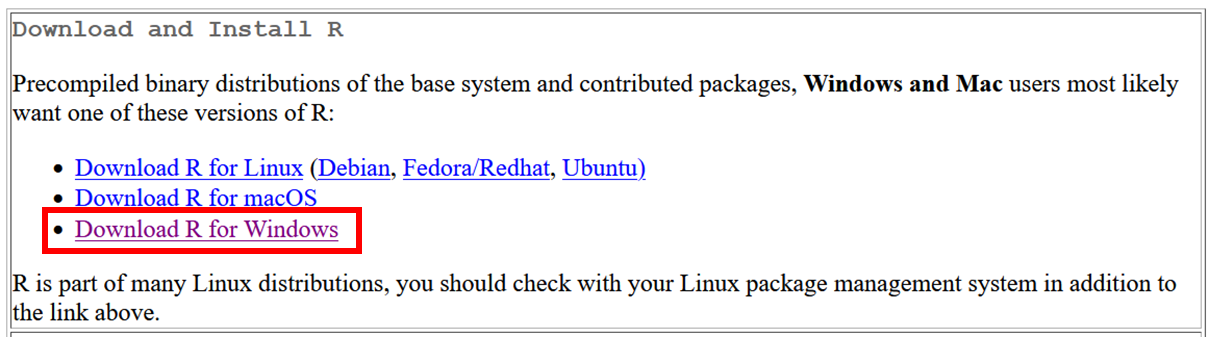
\includegraphics{./images/paste-23A4B16E.png}

\hypertarget{step-3-1}{%
\subsubsection{Step 3}\label{step-3-1}}

Select binaries for base distribution

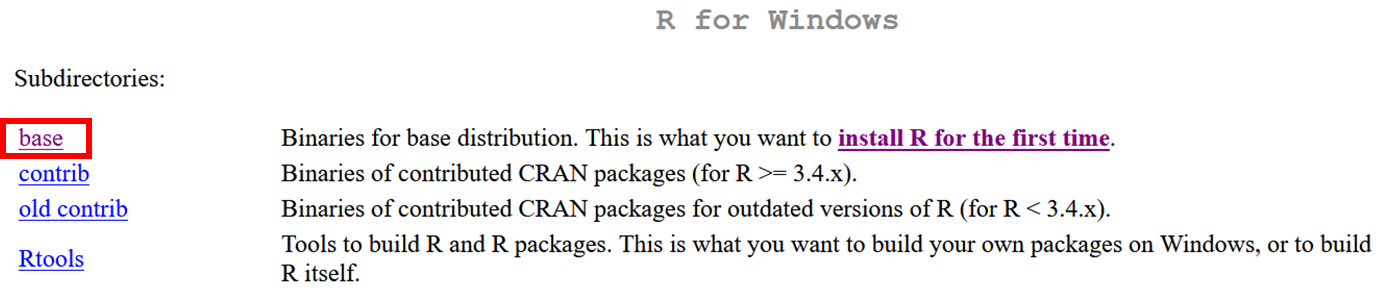
\includegraphics{./images/paste-0739A4C1.png}

\hypertarget{step-4}{%
\subsubsection{Step 4}\label{step-4}}

Download the R installer (\textless{} 80 MB)

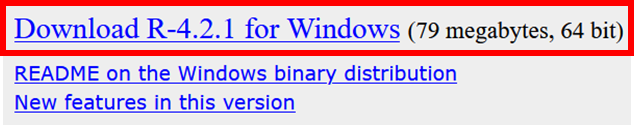
\includegraphics[width=3.64583in,height=\textheight]{./images/paste-9624855F.png}

\hypertarget{step-5}{%
\subsubsection{Step 5}\label{step-5}}

In your computer's Downloads folder, double-click the R setup file.


\includegraphics{./images/paste-FD7C97A4.png}

\hypertarget{step-6}{%
\subsubsection{Step 6}\label{step-6}}

Follow the instruction in the installation wizard to complete the
installation.

\includegraphics{./images/paste-0F242DBF.png}

\hypertarget{sec-RStudio-installation}{%
\section{Install and setup RStudio
Desktop}\label{sec-RStudio-installation}}

\textbf{Rstudio} is an integrated development environment (IDE) for R
that enables an easier use of R.

\begin{tcolorbox}[enhanced jigsaw, colframe=quarto-callout-note-color-frame, colback=white, rightrule=.15mm, bottomrule=.15mm, left=2mm, arc=.35mm, coltitle=black, title=\textcolor{quarto-callout-note-color}{\faInfo}\hspace{0.5em}{Note}, opacitybacktitle=0.6, bottomtitle=1mm, opacityback=0, toptitle=1mm, toprule=.15mm, colbacktitle=quarto-callout-note-color!10!white, titlerule=0mm, leftrule=.75mm, breakable]
RStudio is moving away from its R-exclusive focus and becoming
\href{https://posit.co/}{Posit} in October 2022 to enable broader data
science, scientific research, and technical communication
functionalities and, in particular, to integrate Python users.
\end{tcolorbox}

\begin{tcolorbox}[enhanced jigsaw, colframe=quarto-callout-important-color-frame, colback=white, rightrule=.15mm, bottomrule=.15mm, left=2mm, arc=.35mm, coltitle=black, title=\textcolor{quarto-callout-important-color}{\faExclamation}\hspace{0.5em}{Important}, opacitybacktitle=0.6, bottomtitle=1mm, opacityback=0, toptitle=1mm, toprule=.15mm, colbacktitle=quarto-callout-important-color!10!white, titlerule=0mm, leftrule=.75mm, breakable]
In order for RStudio desktop to work with R you must have installed R on
your computer, see \textbf{?@sec-R-installation}. RStudio does not
include R when you download and install it.
\end{tcolorbox}

\hypertarget{step-1-2}{%
\subsubsection{Step 1}\label{step-1-2}}

You can download R from the
\href{https://www.rstudio.com/products/rstudio/download/}{RStudio
website}. There are different RStudio products available, but the free
Desktop version offers all necessary features for your analyses.

\includegraphics{./images/paste-3C3D0718.png}

\hypertarget{step-2-2}{%
\subsubsection{Step 2}\label{step-2-2}}

\includegraphics{./images/paste-027BCBD8.png}

Download the RStudio Desktop installer that corresponds to your
operating system.

\hypertarget{step-3-2}{%
\subsubsection{Step 3}\label{step-3-2}}

In your computer's Downloads folder, double-click the RStudio Desktop
setup file.

\includegraphics{./images/paste-31A16011.png}

\hypertarget{step-4-1}{%
\subsubsection{Step 4}\label{step-4-1}}

Follow the instruction in the installation wizard to complete the
installation.

\includegraphics{./images/paste-427EA827.png}

\hypertarget{step-5-1}{%
\subsubsection{Step 5}\label{step-5-1}}

Open RStudio

\hypertarget{step-6-1}{%
\subsubsection{Step 6}\label{step-6-1}}

In RStudio, you can set global options by selecting \textbf{Tools}
\textgreater{} \textbf{Global options}

\includegraphics{./images/paste-D0B6CCF0.png}

\hypertarget{step-7}{%
\subsubsection{Step 7}\label{step-7}}

Under the \textbf{General} options and the \textbf{Basic} tab:

\begin{itemize}
\tightlist
\item
  \textbf{Workspace}

  \begin{itemize}
  \item
    Uncheck \emph{Restore .RData into workspace at startup}
  \item
    Ensure that \emph{Never} is selected for \emph{Save workspace to
    .RData on exit}.
  \end{itemize}
\item
  \textbf{History}

  \begin{itemize}
  \item
    Uncheck \emph{Always save history (even when not saving .RData)}
  \item
    Uncheck \emph{Remove duplicate entries in history}
  \end{itemize}
\end{itemize}

\includegraphics{./images/paste-A507B21D.png}

\hypertarget{sec-Quarto-installation}{%
\section{Install Quarto}\label{sec-Quarto-installation}}

\textbf{Quarto} is a software tool that allows to generate high quality
reproducible data analysis documents (including but not limited to
articles, reports, presentations) with programming language used in data
science (such as R, Python or Julia). It is the successor to \textbf{R
Markdown}.

\hypertarget{step-1-3}{%
\subsubsection{Step 1}\label{step-1-3}}

You can download the Quarto installer that corresponds to your operating
system from the \href{https://quarto.org/docs/get-started/}{Quarto
website}.

\includegraphics{./images/paste-DDD0332C.png}

\hypertarget{step-2-3}{%
\subsubsection{Step 2}\label{step-2-3}}

1. In your computer's Downloads folder, double-click the Quarto setup
file.

2. Follow the instruction in the installation wizard to complete the
installation.

\includegraphics{./images/paste-FE57875E.png}

\begin{tcolorbox}[enhanced jigsaw, colframe=quarto-callout-important-color-frame, colback=white, rightrule=.15mm, bottomrule=.15mm, left=2mm, arc=.35mm, coltitle=black, title=\textcolor{quarto-callout-important-color}{\faExclamation}\hspace{0.5em}{Important}, opacitybacktitle=0.6, bottomtitle=1mm, opacityback=0, toptitle=1mm, toprule=.15mm, colbacktitle=quarto-callout-important-color!10!white, titlerule=0mm, leftrule=.75mm, breakable]
When the installation of Quarto is complete, you will not see any new
software on your computer, but Quarto is now available to be used in
RStudio, as well as by all other applications on your computer.

Quarto will select a version of R by looking on your system PATH. Note
that it is possible to override the version of R used by Quarto by
setting the \texttt{QUARTO\_R} environment variable.
\end{tcolorbox}

\hypertarget{sec-rmarkdown-installation}{%
\section{Install the rmarkdown R
package}\label{sec-rmarkdown-installation}}

To use Quarto with R and RStudio, you need to install the
\textbf{rmarkdown} R package.

\begin{tcolorbox}[enhanced jigsaw, colframe=quarto-callout-note-color-frame, colback=white, rightrule=.15mm, bottomrule=.15mm, left=2mm, arc=.35mm, coltitle=black, title=\textcolor{quarto-callout-note-color}{\faInfo}\hspace{0.5em}{Note}, opacitybacktitle=0.6, bottomtitle=1mm, opacityback=0, toptitle=1mm, toprule=.15mm, colbacktitle=quarto-callout-note-color!10!white, titlerule=0mm, leftrule=.75mm, breakable]
A \textbf{R package} is a collection of functions, data, and compiled
code in a well-defined format, created to add specific functionality to
R.

There are 10,000+ user contributed packages and growing.

There is a set of standard (or base) packages which is considered part
of the R source code and automatically available as part of your R
installation. Base packages contain the basic functions that allow R to
work, and enable standard statistical and graphical functions on data
sets.
\end{tcolorbox}

The \textbf{rmarkdown} package will add all necessary functionalities in
your R installation to render Quarto documents that use R.

\hypertarget{step-1-4}{%
\subsubsection{Step 1}\label{step-1-4}}

Open RStudio on your computer

\hypertarget{step-2-4}{%
\subsubsection{Step 2}\label{step-2-4}}

In RStudio, you can install a new package by selecting \textbf{Tools}
\textgreater{} \textbf{Install packages\ldots{}}

\includegraphics{./images/paste-100922E2.png}

\hypertarget{step-3-3}{%
\subsubsection{Step 3}\label{step-3-3}}

\includegraphics{./images/paste-BE660336.png}

\hypertarget{github-setup}{%
\chapter{GitHub setup}\label{github-setup}}

\textbf{GitHub} is a cloud-based hosting platform that lets you host and
manage repositories for version control and collaboration.

\includegraphics[width=2.60417in,height=\textheight]{./images/paste-15A58C67.png}

To Create a GitHub account, follow the instructions that are given in
slide 3 of the Powerpoint document available at the following
\href{https://drive.switch.ch/index.php/s/1eFnksrX0UtjfZV}{link}.

\hypertarget{sec-GitHub-Desktop-installation}{%
\section{Install GitHub desktop}\label{sec-GitHub-Desktop-installation}}

\textbf{GitHub Desktop} is an application that allows to interact with
GitHub through a visual interface instead of using the command line (for
software developers) or GitHub's web browser.

\includegraphics[width=2.60417in,height=\textheight]{./images/paste-9238B1AB.png}

You can install GitHub Desktop on supported Windows or macOS operating
systems.

\hypertarget{step-1-5}{%
\subsubsection{Step 1}\label{step-1-5}}

\begin{enumerate}
\def\labelenumi{\arabic{enumi}.}
\tightlist
\item
  Visit the \href{https://desktop.github.com/}{download page} for GitHub
  Desktop.
\item
  Click Download for Windows.
\end{enumerate}

\includegraphics{./images/paste-465BAC3C.png}

\hypertarget{step-2-5}{%
\subsubsection{Step 2}\label{step-2-5}}

\begin{enumerate}
\def\labelenumi{\arabic{enumi}.}
\tightlist
\item
  In your computer's Downloads folder, double-click the GitHub Desktop
  setup file.
\item
  Follow the instruction in the installation wizard to complete the
  installation.
\end{enumerate}

\hypertarget{step-3-4}{%
\subsubsection{Step 3}\label{step-3-4}}

To connect your GitHub account to GitHub Desktop, follow the
instructions that are given in slides 6 to 9 of the Powerpoint document
available at the following
\href{https://drive.switch.ch/index.php/s/1eFnksrX0UtjfZV}{link}.

\hypertarget{import-data-from-odk-central}{%
\chapter{Import data from ODK
Central}\label{import-data-from-odk-central}}

\hypertarget{overview-8}{%
\subsection{Overview}\label{overview-8}}

Application Programming Interfaces (APIs) allow you to import data
directly from servers.

\hypertarget{learning-objectives-9}{%
\subsection{Learning objectives}\label{learning-objectives-9}}

\begin{itemize}
\tightlist
\item
  We will explore the use of APIs through the example of \textbf{ruODK}
  for importing data from ODK Central to R.
\end{itemize}

\hypertarget{tutorial}{%
\section{Tutorial}\label{tutorial}}

While data digitally captured using ODK Collect or Enketo and stored in
ODK Central can be retrieved in bulk through the web interface, ODK
Central's API provides direct access to its data (and functionality). It
is a more efficient way to ensure that data are always up-to-date.

We will see how to retrieve data through the OData API.

\hypertarget{exercise-1-2}{%
\subsubsection{\texorpdfstring{{✏️} Exercise
1}{✏️ Exercise 1}}\label{exercise-1-2}}

Connect to the ODK Central server data set.

\begin{itemize}
\tightlist
\item
  odata service:
  ``https://private-anon-24fcfe2426-odkcentral.apiary-mock.com/v1/projects/7/forms/simple.svc''
\item
  Email: ``my.email.address@getodk.org''
\item
  Password: ``my.super.secure.password''.
\end{itemize}

\begin{tcolorbox}[enhanced jigsaw, colframe=quarto-callout-tip-color-frame, colback=white, rightrule=.15mm, bottomrule=.15mm, left=2mm, arc=.35mm, coltitle=black, title=\textcolor{quarto-callout-tip-color}{\faLightbulb}\hspace{0.5em}{Tip}, opacitybacktitle=0.6, bottomtitle=1mm, opacityback=0, toptitle=1mm, toprule=.15mm, colbacktitle=quarto-callout-tip-color!10!white, titlerule=0mm, leftrule=.75mm, breakable]

\begin{itemize}
\tightlist
\item
  R: use the
  \href{https://docs.ropensci.org/ruODK/reference/ru_setup.html}{ru\_setup}
  function from the \texttt{ruODK} package (9).
\item
  Python: use functions from the \texttt{pyODK} package.
\end{itemize}

\end{tcolorbox}

\begin{Shaded}
\begin{Highlighting}[]
\InformationTok{\textasciigrave{}\textasciigrave{}\textasciigrave{}\{r\}}
\CommentTok{\# Write your code here}
\InformationTok{\textasciigrave{}\textasciigrave{}\textasciigrave{}}
\end{Highlighting}
\end{Shaded}

\hypertarget{r-4}{%
\subsubsection{R}\label{r-4}}

\begin{Shaded}
\begin{Highlighting}[]
\InformationTok{\textasciigrave{}\textasciigrave{}\textasciigrave{}\{r\}}
\NormalTok{ruODK}\SpecialCharTok{::}\FunctionTok{ru\_setup}\NormalTok{(}
  \AttributeTok{svc =} \StringTok{"https://private{-}anon{-}24fcfe2426{-}odkcentral.apiary{-}mock.com/v1/projects/7/forms/simple.svc"}\NormalTok{,}
  \AttributeTok{un =} \StringTok{"my.email.address@getodk.org"}\NormalTok{,}
  \AttributeTok{pw =} \StringTok{"my.super.secure.password"}\NormalTok{,}
  \AttributeTok{verbose =} \ConstantTok{TRUE}
\NormalTok{)}
\InformationTok{\textasciigrave{}\textasciigrave{}\textasciigrave{}}
\end{Highlighting}
\end{Shaded}

\begin{verbatim}
<ruODK settings>
  Default ODK Central Project ID: 7 
  Default ODK Central Form ID: simple 
  Default ODK Central URL: https://private-anon-24fcfe2426-odkcentral.apiary-mock.com 
  Default ODK Central Username: my.email.address@getodk.org 
  Default ODK Central Password: run ruODK::get_default_pw() to show 
  Default ODK Central Passphrase: run ruODK::get_default_pp() to show 
  Default Time Zone: UTC 
  Default ODK Central Version: 1.1 
  Default HTTP GET retries: 3 
  Verbose messages: TRUE 
  Test ODK Central Project ID:  
  Test ODK Central Form ID:  
  Test ODK Central Form ID (ZIP tests):  
  Test ODK Central Form ID (Attachment tests):  
  Test ODK Central Form ID (Parsing tests):  
  Test ODK Central Form ID (WKT tests):  
  Test ODK Central URL:  
  Test ODK Central Username:  
  Test ODK Central Password: run ruODK::get_test_pw() to show 
  Test ODK Central Passphrase: run ruODK::get_test_pp() to show 
  Test ODK Central Version: 1.1 
\end{verbatim}

\hypertarget{exercise-2-1}{%
\subsubsection{\texorpdfstring{{✏️} Exercise
2}{✏️ Exercise 2}}\label{exercise-2-1}}

Retrieve data from form and store the data set into a data frame called
df4

\begin{tcolorbox}[enhanced jigsaw, colframe=quarto-callout-tip-color-frame, colback=white, rightrule=.15mm, bottomrule=.15mm, left=2mm, arc=.35mm, coltitle=black, title=\textcolor{quarto-callout-tip-color}{\faLightbulb}\hspace{0.5em}{Tip}, opacitybacktitle=0.6, bottomtitle=1mm, opacityback=0, toptitle=1mm, toprule=.15mm, colbacktitle=quarto-callout-tip-color!10!white, titlerule=0mm, leftrule=.75mm, breakable]

\begin{itemize}
\tightlist
\item
  R: use the
  \href{https://docs.ropensci.org/ruODK/reference/odata_submission_get.html}{odata\_submission\_get}
  function from the \texttt{ruODK} package (9).
\item
  Python: use functions from the \texttt{pyODK} package.
\end{itemize}

\end{tcolorbox}

\begin{Shaded}
\begin{Highlighting}[]
\InformationTok{\textasciigrave{}\textasciigrave{}\textasciigrave{}\{r\}}
\CommentTok{\# Write your code here}
\InformationTok{\textasciigrave{}\textasciigrave{}\textasciigrave{}}
\end{Highlighting}
\end{Shaded}

\hypertarget{r-5}{%
\subsubsection{R}\label{r-5}}

\begin{Shaded}
\begin{Highlighting}[]
\InformationTok{\textasciigrave{}\textasciigrave{}\textasciigrave{}\{r\}}
\NormalTok{fq\_form\_schema }\OtherTok{\textless{}{-}}\NormalTok{ ruODK}\SpecialCharTok{::}\FunctionTok{form\_schema}\NormalTok{()}
\InformationTok{\textasciigrave{}\textasciigrave{}\textasciigrave{}}
\end{Highlighting}
\end{Shaded}

\begin{verbatim}
i Form schema v1.1
\end{verbatim}

\begin{Shaded}
\begin{Highlighting}[]
\InformationTok{\textasciigrave{}\textasciigrave{}\textasciigrave{}\{r\}}
\NormalTok{fq\_form\_schema}
\InformationTok{\textasciigrave{}\textasciigrave{}\textasciigrave{}}
\end{Highlighting}
\end{Shaded}

\begin{verbatim}
# A tibble: 5 x 5
  name       path             type      binary ruodk_name      
  <chr>      <chr>            <chr>     <lgl>  <chr>           
1 meta       /meta            structure NA     meta            
2 instanceID /meta/instanceID string    NA     meta_instance_id
3 name       /name            string    NA     name            
4 age        /age             int       NA     age             
5 photo      /photo           binary    TRUE   photo           
\end{verbatim}

\begin{Shaded}
\begin{Highlighting}[]
\InformationTok{\textasciigrave{}\textasciigrave{}\textasciigrave{}\{r\}}
\NormalTok{df }\OtherTok{\textless{}{-}}\NormalTok{ ruODK}\SpecialCharTok{::}\FunctionTok{odata\_service\_get}\NormalTok{()}
\NormalTok{df}
\InformationTok{\textasciigrave{}\textasciigrave{}\textasciigrave{}}
\end{Highlighting}
\end{Shaded}

\begin{verbatim}
# A tibble: 0 x 3
# ... with 3 variables: name <chr>, kind <chr>, url <chr>
\end{verbatim}

\hypertarget{encrypted-data}{%
\section{Encrypted data}\label{encrypted-data}}

Encrypted data can only be retrieved using the RESTful API and cannot be
retrieved using the oData API. ODK Central supports two modes of
encryption - learn about them here. ruODK supports project managed
encryption, however the support is limited to exactly one encryption
key. The supplied passphrase will be used against the first returned
encryption key. Remaining encryption keys are ignored by ruODK.

\begin{tcolorbox}[enhanced jigsaw, colframe=quarto-callout-important-color-frame, colback=white, rightrule=.15mm, bottomrule=.15mm, left=2mm, arc=.35mm, coltitle=black, title=\textcolor{quarto-callout-important-color}{\faExclamation}\hspace{0.5em}{Important}, opacitybacktitle=0.6, bottomtitle=1mm, opacityback=0, toptitle=1mm, toprule=.15mm, colbacktitle=quarto-callout-important-color!10!white, titlerule=0mm, leftrule=.75mm, breakable]
If an incorrect passphrase is given, the request is terminated
immediately. It has been reported that multiple requests with incorrect
passphrases can crash ODK Central.
\end{tcolorbox}

\hypertarget{sec-useful-resources}{%
\chapter{Useful resources}\label{sec-useful-resources}}

\hypertarget{reproducible-research}{%
\section{Reproducible research}\label{reproducible-research}}

\begin{itemize}
\tightlist
\item
  \href{https://the-turing-way.netlify.app/welcome.html}{The Turing way}
  (1) {⭐} {⭐} {⭐} {⭐} {⭐}
\end{itemize}

\hypertarget{sec-resources-git}{%
\section{Git and GitHub}\label{sec-resources-git}}

To learn more about this topic, we highly recommend the following
resources:

\begin{itemize}
\tightlist
\item
  \href{https://www.codecademy.com/learn/learn-git}{Codeacademy}
\item
  \href{https://guides.github.com/activities/hello-world/}{GitHub
  Guides}
\item
  \href{https://try.github.io/levels/1/challenges/1}{Try Git tutorial}
\item
  \href{http://happygitwithr.com/}{Happy Git and GitHub for the useR}
\end{itemize}

\hypertarget{online-trainings}{%
\section{Online trainings}\label{online-trainings}}

\hypertarget{programming}{%
\subsection{Programming}\label{programming}}

\begin{longtable}[]{@{}
  >{\raggedright\arraybackslash}p{(\columnwidth - 4\tabcolsep) * \real{0.6400}}
  >{\raggedright\arraybackslash}p{(\columnwidth - 4\tabcolsep) * \real{0.1200}}
  >{\raggedright\arraybackslash}p{(\columnwidth - 4\tabcolsep) * \real{0.2400}}@{}}
\toprule()
\begin{minipage}[b]{\linewidth}\raggedright
Link
\end{minipage} & \begin{minipage}[b]{\linewidth}\raggedright
Language
\end{minipage} & \begin{minipage}[b]{\linewidth}\raggedright
Recommendation
\end{minipage} \\
\midrule()
\endhead
\href{https://thegraphcourses.org}{The GRAPH network} & R & {⭐} {⭐}
{⭐} {⭐} {⭐} \\
\href{https://jhudatascience.org/courses.html}{Johns Hopkins University
Data Science Lab's courses} & R & {⭐} {⭐} {⭐} {⭐} {⭐} \\
\href{https://afrimapr.github.io/afrimapr.website/training/}{afrimapr} -
mapping data in Africa & R & \\
\href{https://iqss.github.io/dss-workshops/}{Harvard Data Science
workshops materials} & R, Python, Stata & \\
\bottomrule()
\end{longtable}

\hypertarget{machine-learning}{%
\subsection{Machine learning}\label{machine-learning}}

\begin{longtable}[]{@{}
  >{\raggedright\arraybackslash}p{(\columnwidth - 4\tabcolsep) * \real{0.7262}}
  >{\raggedright\arraybackslash}p{(\columnwidth - 4\tabcolsep) * \real{0.0595}}
  >{\raggedright\arraybackslash}p{(\columnwidth - 4\tabcolsep) * \real{0.2143}}@{}}
\toprule()
\begin{minipage}[b]{\linewidth}\raggedright
MOOC
\end{minipage} & \begin{minipage}[b]{\linewidth}\raggedright
Language
\end{minipage} & \begin{minipage}[b]{\linewidth}\raggedright
Recommendation
\end{minipage} \\
\midrule()
\endhead
\href{https://www.fun-mooc.fr/en/courses/machine-learning-python-scikit-learn/}{Machine
learning in Python with scikit-learn} & Python & {⭐} {⭐} {⭐} {⭐}
{⭐} \\
\bottomrule()
\end{longtable}

\hypertarget{packages}{%
\section{Packages}\label{packages}}

\hypertarget{r-6}{%
\subsection{R}\label{r-6}}

\begin{longtable}[]{@{}
  >{\raggedright\arraybackslash}p{(\columnwidth - 4\tabcolsep) * \real{0.2586}}
  >{\raggedright\arraybackslash}p{(\columnwidth - 4\tabcolsep) * \real{0.4425}}
  >{\raggedright\arraybackslash}p{(\columnwidth - 4\tabcolsep) * \real{0.2989}}@{}}
\toprule()
\endhead
\includegraphics[width=1.30208in,height=\textheight]{./images/tidyverse-logo.png}
& \href{https://www.tidyverse.org/}{tidyverse} & Collection of R
packages designed for data science \\
\includegraphics[width=1.30208in,height=\textheight]{./images/logo.png}
& \href{https://docs.ropensci.org/ruODK/index.html}{ruODK} & \\
\includegraphics[width=1.30208in,height=\textheight]{./images/logo-01.png}
& \href{https://www.danieldsjoberg.com/gtsummary/}{gtsummary} & \\
\includegraphics[width=1.30208in,height=\textheight]{./images/paste-A6E65357.png}
&
\href{https://cran.r-project.org/web/packages/skimr/vignettes/skimr.html}{skimr}
& \\
& \href{https://github.com/R4EPI/sitrep}{sitrep} & \\
\bottomrule()
\end{longtable}

\hypertarget{python-4}{%
\subsection{Python}\label{python-4}}

\begin{itemize}
\tightlist
\item
  \textbf{Pandas}\\
  \href{https://pandas.pydata.org/docs/getting_started/comparison/comparison_with_stata.html}{Comparison
  with Stata}\\
  \href{https://pandas.pydata.org/docs/getting_started/comparison/comparison_with_r.html}{Comparison
  with R}
\end{itemize}

\hypertarget{books-and-websites}{%
\section{Books and websites}\label{books-and-websites}}

\begin{longtable}[]{@{}
  >{\raggedright\arraybackslash}p{(\columnwidth - 2\tabcolsep) * \real{0.7483}}
  >{\raggedright\arraybackslash}p{(\columnwidth - 2\tabcolsep) * \real{0.2517}}@{}}
\caption{Books and websites}\tabularnewline
\toprule()
\endhead
\href{https://epirhandbook.com/en/}{R for applied epidemiology and
public health} (10) & {⭐} {⭐} {⭐} {⭐} {⭐} \\
\href{https://www.r4epi.com/}{R for Epidemiology} & \\
\href{https://r4epis.netlify.app/}{R4epis} & \\
\href{https://r4ds.had.co.nz/}{R for Data Science} & {⭐} {⭐} {⭐} {⭐}
{⭐} \\
\href{https://qmd4sci.njtierney.com/}{Quarto for scientists} & \\
\bottomrule()
\end{longtable}

\hypertarget{communities}{%
\section{Communities}\label{communities}}

\begin{itemize}
\tightlist
\item
  \href{https://www.rfordatasci.com/}{R for data science online learning
  community}
\end{itemize}

\hypertarget{open-data}{%
\section{Open data}\label{open-data}}

\hypertarget{platforms}{%
\subsection{Platforms}\label{platforms}}

\begin{itemize}
\item
  \href{https://open.africa/}{openAfrica}
\item
  \href{https://github.com/CodeForAfrica/}{Code for Africa (CfA)}
\end{itemize}

\hypertarget{data-sets}{%
\subsection{Data sets}\label{data-sets}}

\begin{longtable}[]{@{}
  >{\raggedright\arraybackslash}p{(\columnwidth - 2\tabcolsep) * \real{0.7985}}
  >{\raggedright\arraybackslash}p{(\columnwidth - 2\tabcolsep) * \real{0.2015}}@{}}
\toprule()
\begin{minipage}[b]{\linewidth}\raggedright
Dataset
\end{minipage} & \begin{minipage}[b]{\linewidth}\raggedright
Associated publication(s)
\end{minipage} \\
\midrule()
\endhead
\href{https://dataforgood.facebook.com/dfg/tools}{Data for Good} & \\
\href{https://open.africa/dataset/health-facilities-in-africa}{Public
health hacilities in sub-Saharan Africa} & (5) \\
\bottomrule()
\end{longtable}

\hypertarget{conferences}{%
\section{Conferences}\label{conferences}}

\begin{itemize}
\item
  \href{http://www.datascienceafrica.org/}{Data Science Africa}
\item
  https://nef.org/
\end{itemize}



\end{document}
